% Options for packages loaded elsewhere
\PassOptionsToPackage{unicode}{hyperref}
\PassOptionsToPackage{hyphens}{url}
\PassOptionsToPackage{dvipsnames,svgnames,x11names}{xcolor}
%
\documentclass[
  letterpaper,
  DIV=11,
  numbers=noendperiod]{scrreprt}

\usepackage{amsmath,amssymb}
\usepackage{iftex}
\ifPDFTeX
  \usepackage[T1]{fontenc}
  \usepackage[utf8]{inputenc}
  \usepackage{textcomp} % provide euro and other symbols
\else % if luatex or xetex
  \usepackage{unicode-math}
  \defaultfontfeatures{Scale=MatchLowercase}
  \defaultfontfeatures[\rmfamily]{Ligatures=TeX,Scale=1}
\fi
\usepackage{lmodern}
\ifPDFTeX\else  
    % xetex/luatex font selection
\fi
% Use upquote if available, for straight quotes in verbatim environments
\IfFileExists{upquote.sty}{\usepackage{upquote}}{}
\IfFileExists{microtype.sty}{% use microtype if available
  \usepackage[]{microtype}
  \UseMicrotypeSet[protrusion]{basicmath} % disable protrusion for tt fonts
}{}
\makeatletter
\@ifundefined{KOMAClassName}{% if non-KOMA class
  \IfFileExists{parskip.sty}{%
    \usepackage{parskip}
  }{% else
    \setlength{\parindent}{0pt}
    \setlength{\parskip}{6pt plus 2pt minus 1pt}}
}{% if KOMA class
  \KOMAoptions{parskip=half}}
\makeatother
\usepackage{xcolor}
\setlength{\emergencystretch}{3em} % prevent overfull lines
\setcounter{secnumdepth}{5}
% Make \paragraph and \subparagraph free-standing
\ifx\paragraph\undefined\else
  \let\oldparagraph\paragraph
  \renewcommand{\paragraph}[1]{\oldparagraph{#1}\mbox{}}
\fi
\ifx\subparagraph\undefined\else
  \let\oldsubparagraph\subparagraph
  \renewcommand{\subparagraph}[1]{\oldsubparagraph{#1}\mbox{}}
\fi

\usepackage{color}
\usepackage{fancyvrb}
\newcommand{\VerbBar}{|}
\newcommand{\VERB}{\Verb[commandchars=\\\{\}]}
\DefineVerbatimEnvironment{Highlighting}{Verbatim}{commandchars=\\\{\}}
% Add ',fontsize=\small' for more characters per line
\usepackage{framed}
\definecolor{shadecolor}{RGB}{241,243,245}
\newenvironment{Shaded}{\begin{snugshade}}{\end{snugshade}}
\newcommand{\AlertTok}[1]{\textcolor[rgb]{0.68,0.00,0.00}{#1}}
\newcommand{\AnnotationTok}[1]{\textcolor[rgb]{0.37,0.37,0.37}{#1}}
\newcommand{\AttributeTok}[1]{\textcolor[rgb]{0.40,0.45,0.13}{#1}}
\newcommand{\BaseNTok}[1]{\textcolor[rgb]{0.68,0.00,0.00}{#1}}
\newcommand{\BuiltInTok}[1]{\textcolor[rgb]{0.00,0.23,0.31}{#1}}
\newcommand{\CharTok}[1]{\textcolor[rgb]{0.13,0.47,0.30}{#1}}
\newcommand{\CommentTok}[1]{\textcolor[rgb]{0.37,0.37,0.37}{#1}}
\newcommand{\CommentVarTok}[1]{\textcolor[rgb]{0.37,0.37,0.37}{\textit{#1}}}
\newcommand{\ConstantTok}[1]{\textcolor[rgb]{0.56,0.35,0.01}{#1}}
\newcommand{\ControlFlowTok}[1]{\textcolor[rgb]{0.00,0.23,0.31}{#1}}
\newcommand{\DataTypeTok}[1]{\textcolor[rgb]{0.68,0.00,0.00}{#1}}
\newcommand{\DecValTok}[1]{\textcolor[rgb]{0.68,0.00,0.00}{#1}}
\newcommand{\DocumentationTok}[1]{\textcolor[rgb]{0.37,0.37,0.37}{\textit{#1}}}
\newcommand{\ErrorTok}[1]{\textcolor[rgb]{0.68,0.00,0.00}{#1}}
\newcommand{\ExtensionTok}[1]{\textcolor[rgb]{0.00,0.23,0.31}{#1}}
\newcommand{\FloatTok}[1]{\textcolor[rgb]{0.68,0.00,0.00}{#1}}
\newcommand{\FunctionTok}[1]{\textcolor[rgb]{0.28,0.35,0.67}{#1}}
\newcommand{\ImportTok}[1]{\textcolor[rgb]{0.00,0.46,0.62}{#1}}
\newcommand{\InformationTok}[1]{\textcolor[rgb]{0.37,0.37,0.37}{#1}}
\newcommand{\KeywordTok}[1]{\textcolor[rgb]{0.00,0.23,0.31}{#1}}
\newcommand{\NormalTok}[1]{\textcolor[rgb]{0.00,0.23,0.31}{#1}}
\newcommand{\OperatorTok}[1]{\textcolor[rgb]{0.37,0.37,0.37}{#1}}
\newcommand{\OtherTok}[1]{\textcolor[rgb]{0.00,0.23,0.31}{#1}}
\newcommand{\PreprocessorTok}[1]{\textcolor[rgb]{0.68,0.00,0.00}{#1}}
\newcommand{\RegionMarkerTok}[1]{\textcolor[rgb]{0.00,0.23,0.31}{#1}}
\newcommand{\SpecialCharTok}[1]{\textcolor[rgb]{0.37,0.37,0.37}{#1}}
\newcommand{\SpecialStringTok}[1]{\textcolor[rgb]{0.13,0.47,0.30}{#1}}
\newcommand{\StringTok}[1]{\textcolor[rgb]{0.13,0.47,0.30}{#1}}
\newcommand{\VariableTok}[1]{\textcolor[rgb]{0.07,0.07,0.07}{#1}}
\newcommand{\VerbatimStringTok}[1]{\textcolor[rgb]{0.13,0.47,0.30}{#1}}
\newcommand{\WarningTok}[1]{\textcolor[rgb]{0.37,0.37,0.37}{\textit{#1}}}

\providecommand{\tightlist}{%
  \setlength{\itemsep}{0pt}\setlength{\parskip}{0pt}}\usepackage{longtable,booktabs,array}
\usepackage{calc} % for calculating minipage widths
% Correct order of tables after \paragraph or \subparagraph
\usepackage{etoolbox}
\makeatletter
\patchcmd\longtable{\par}{\if@noskipsec\mbox{}\fi\par}{}{}
\makeatother
% Allow footnotes in longtable head/foot
\IfFileExists{footnotehyper.sty}{\usepackage{footnotehyper}}{\usepackage{footnote}}
\makesavenoteenv{longtable}
\usepackage{graphicx}
\makeatletter
\def\maxwidth{\ifdim\Gin@nat@width>\linewidth\linewidth\else\Gin@nat@width\fi}
\def\maxheight{\ifdim\Gin@nat@height>\textheight\textheight\else\Gin@nat@height\fi}
\makeatother
% Scale images if necessary, so that they will not overflow the page
% margins by default, and it is still possible to overwrite the defaults
% using explicit options in \includegraphics[width, height, ...]{}
\setkeys{Gin}{width=\maxwidth,height=\maxheight,keepaspectratio}
% Set default figure placement to htbp
\makeatletter
\def\fps@figure{htbp}
\makeatother
\newlength{\cslhangindent}
\setlength{\cslhangindent}{1.5em}
\newlength{\csllabelwidth}
\setlength{\csllabelwidth}{3em}
\newlength{\cslentryspacingunit} % times entry-spacing
\setlength{\cslentryspacingunit}{\parskip}
\newenvironment{CSLReferences}[2] % #1 hanging-ident, #2 entry spacing
 {% don't indent paragraphs
  \setlength{\parindent}{0pt}
  % turn on hanging indent if param 1 is 1
  \ifodd #1
  \let\oldpar\par
  \def\par{\hangindent=\cslhangindent\oldpar}
  \fi
  % set entry spacing
  \setlength{\parskip}{#2\cslentryspacingunit}
 }%
 {}
\usepackage{calc}
\newcommand{\CSLBlock}[1]{#1\hfill\break}
\newcommand{\CSLLeftMargin}[1]{\parbox[t]{\csllabelwidth}{#1}}
\newcommand{\CSLRightInline}[1]{\parbox[t]{\linewidth - \csllabelwidth}{#1}\break}
\newcommand{\CSLIndent}[1]{\hspace{\cslhangindent}#1}

\KOMAoption{captions}{tableheading}
\makeatletter
\makeatother
\makeatletter
\@ifpackageloaded{bookmark}{}{\usepackage{bookmark}}
\makeatother
\makeatletter
\@ifpackageloaded{caption}{}{\usepackage{caption}}
\AtBeginDocument{%
\ifdefined\contentsname
  \renewcommand*\contentsname{Table of contents}
\else
  \newcommand\contentsname{Table of contents}
\fi
\ifdefined\listfigurename
  \renewcommand*\listfigurename{List of Figures}
\else
  \newcommand\listfigurename{List of Figures}
\fi
\ifdefined\listtablename
  \renewcommand*\listtablename{List of Tables}
\else
  \newcommand\listtablename{List of Tables}
\fi
\ifdefined\figurename
  \renewcommand*\figurename{Figure}
\else
  \newcommand\figurename{Figure}
\fi
\ifdefined\tablename
  \renewcommand*\tablename{Table}
\else
  \newcommand\tablename{Table}
\fi
}
\@ifpackageloaded{float}{}{\usepackage{float}}
\floatstyle{ruled}
\@ifundefined{c@chapter}{\newfloat{codelisting}{h}{lop}}{\newfloat{codelisting}{h}{lop}[chapter]}
\floatname{codelisting}{Listing}
\newcommand*\listoflistings{\listof{codelisting}{List of Listings}}
\makeatother
\makeatletter
\@ifpackageloaded{caption}{}{\usepackage{caption}}
\@ifpackageloaded{subcaption}{}{\usepackage{subcaption}}
\makeatother
\makeatletter
\@ifpackageloaded{tcolorbox}{}{\usepackage[skins,breakable]{tcolorbox}}
\makeatother
\makeatletter
\@ifundefined{shadecolor}{\definecolor{shadecolor}{rgb}{.97, .97, .97}}
\makeatother
\makeatletter
\makeatother
\makeatletter
\makeatother
\ifLuaTeX
  \usepackage{selnolig}  % disable illegal ligatures
\fi
\IfFileExists{bookmark.sty}{\usepackage{bookmark}}{\usepackage{hyperref}}
\IfFileExists{xurl.sty}{\usepackage{xurl}}{} % add URL line breaks if available
\urlstyle{same} % disable monospaced font for URLs
\hypersetup{
  pdftitle={Introdução aos modelos lineares dinâmicos},
  pdfauthor={James D Santos},
  colorlinks=true,
  linkcolor={blue},
  filecolor={Maroon},
  citecolor={Blue},
  urlcolor={Blue},
  pdfcreator={LaTeX via pandoc}}

\title{Introdução aos modelos lineares dinâmicos}
\author{James D Santos}
\date{2025-04-09}

\begin{document}
\maketitle
\ifdefined\Shaded\renewenvironment{Shaded}{\begin{tcolorbox}[frame hidden, sharp corners, interior hidden, borderline west={3pt}{0pt}{shadecolor}, boxrule=0pt, enhanced, breakable]}{\end{tcolorbox}}\fi

\renewcommand*\contentsname{Table of contents}
{
\hypersetup{linkcolor=}
\setcounter{tocdepth}{2}
\tableofcontents
}
\bookmarksetup{startatroot}

\hypertarget{prefuxe1cio}{%
\chapter*{Prefácio}\label{prefuxe1cio}}
\addcontentsline{toc}{chapter}{Prefácio}

\markboth{Prefácio}{Prefácio}

\bookmarksetup{startatroot}

\hypertarget{summary}{%
\chapter{Summary}\label{summary}}

In summary, this book has no content whatsoever.

\begin{Shaded}
\begin{Highlighting}[]
\DecValTok{1} \SpecialCharTok{+} \DecValTok{1}
\end{Highlighting}
\end{Shaded}

\begin{verbatim}
[1] 2
\end{verbatim}

\bookmarksetup{startatroot}

\hypertarget{introduuxe7uxe3o}{%
\chapter{Introdução}\label{introduuxe7uxe3o}}

\hypertarget{definiuxe7uxe3o-de-suxe9ries-temporais}{%
\section{Definição de séries
temporais}\label{definiuxe7uxe3o-de-suxe9ries-temporais}}

Considere um fenômeno aleatório que será observado ao longo do tempo. A
coleção de variáveis aleatórias indexadas no tempo associadas a este
fenômeno será denominada série temporal. Neste caso, para cada instante
de tempo \(t\), há uma variável \(X(t)\) associada.

\begin{figure}

{\centering 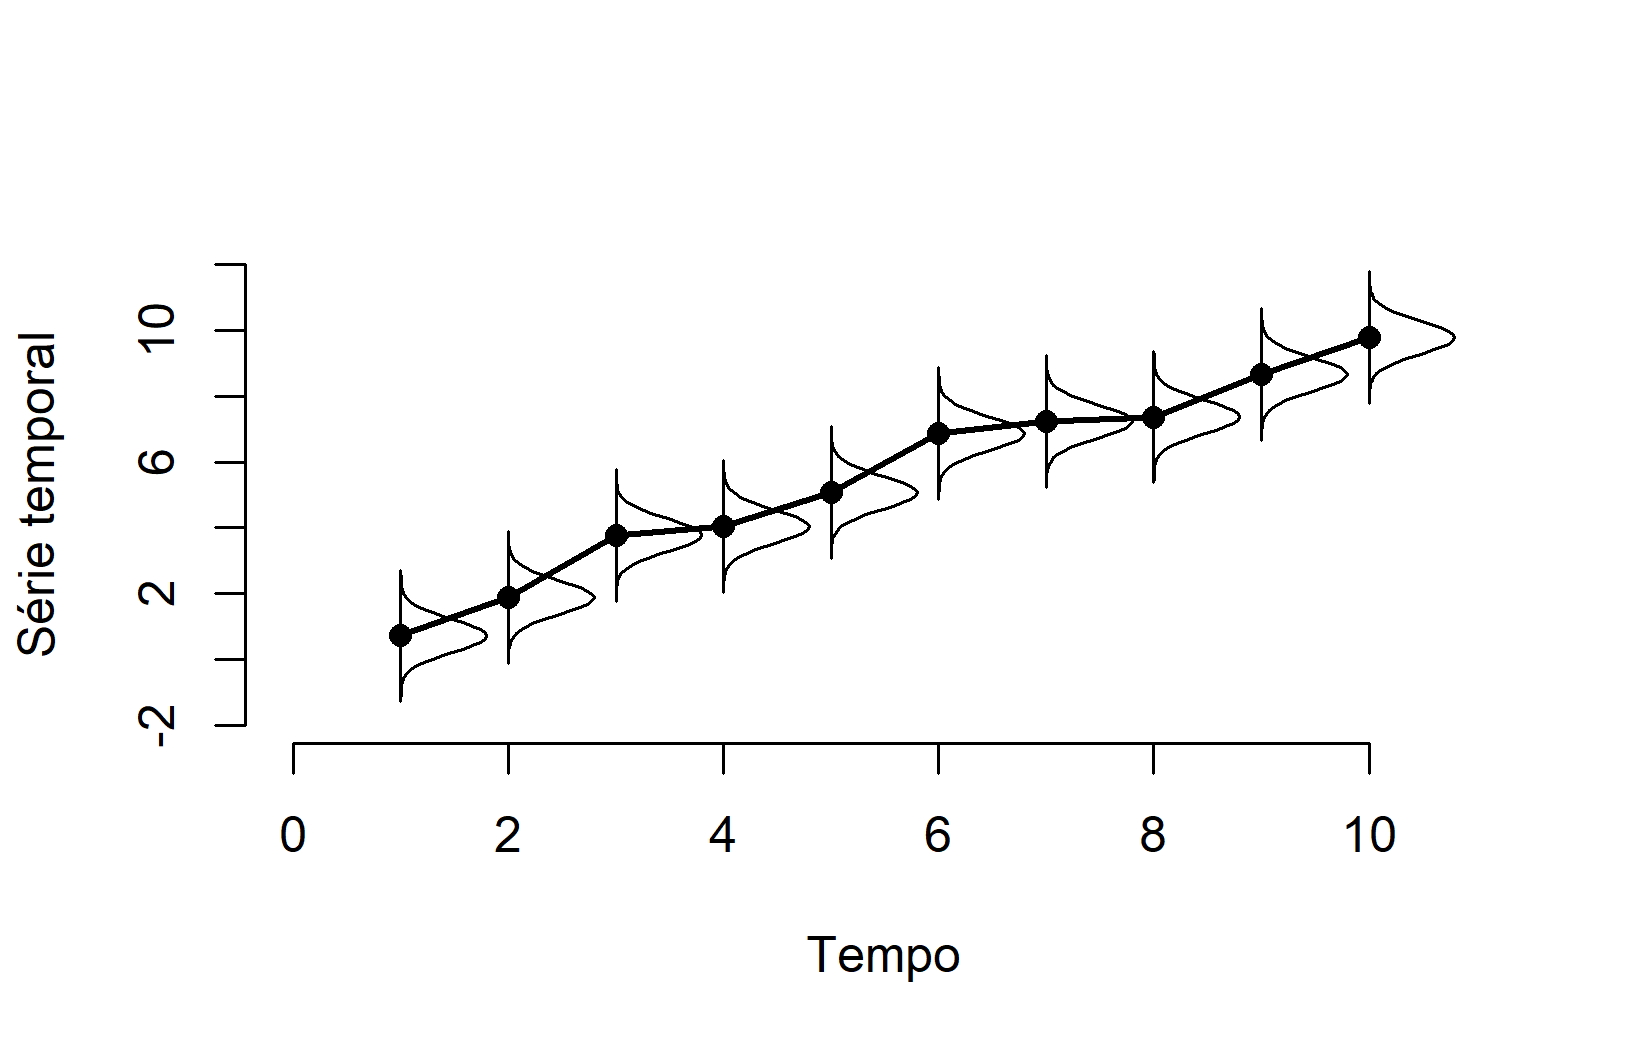
\includegraphics{intro_files/figure-pdf/figura1-1.png}

}

\caption{Figure 1 - Ilustração de uma série temporal}

\end{figure}

Alguns autores definem séries temporais simplesmente como uma os valores
de uma variável registrados ao longo do tempo. Essa definição não é útil
para nós, uma vez que o tempo não necessariamente possui influência na
variável, ou seja, é possível que a distribuição de \(X(t)\) não dependa
de \(t\).

Importante: estamos interessados apenas em séries temporais nas quais o
modelo de probabilidades depende do tempo \(t\).

A partir deste momento, \(X(t)\) será escrita como \(X_t\) e
representará a variável aleatória associada ao tempo \(t\) e a versão
minúscula \(x_t\) representará o valor observado.

\hypertarget{a-classe-ts}{%
\section{\texorpdfstring{A classe
\texttt{ts}}{A classe ts}}\label{a-classe-ts}}

A tabela aabeixo apresenta o número de nascidos vivos por mês na cidade
de Manaus em 2021.

\begin{longtable}[]{@{}ll@{}}
\toprule\noalign{}
Mês & No.~nascidos vivos \\
\midrule\noalign{}
\endhead
\bottomrule\noalign{}
\endlastfoot
Janeiro & 3043 \\
Fevereiro & 2902 \\
Março & 3166 \\
Abril & 3014 \\
Maio & 3095 \\
Junho & 2955 \\
Julho & 3087 \\
Agosto & 3141 \\
Setembro & 3129 \\
Outubro & 3096 \\
Novembro & 3191 \\
Dezembro & 3222 \\
\end{longtable}

Para todos os efeitos, uma série temporal é um vetor numérico.

\begin{Shaded}
\begin{Highlighting}[]
\NormalTok{x }\OtherTok{\textless{}{-}} \FunctionTok{c}\NormalTok{(}
  \DecValTok{3043}\NormalTok{, }\DecValTok{2902}\NormalTok{, }\DecValTok{3166}\NormalTok{, }\DecValTok{3014}\NormalTok{,}
\DecValTok{3095}\NormalTok{, }\DecValTok{2955}\NormalTok{, }\DecValTok{3087}\NormalTok{, }\DecValTok{3141}\NormalTok{,}
\DecValTok{3129}\NormalTok{, }\DecValTok{3096}\NormalTok{, }\DecValTok{3191}\NormalTok{, }\DecValTok{3222}

\NormalTok{)}

\FunctionTok{plot}\NormalTok{(x, }\AttributeTok{type =} \StringTok{\textquotesingle{}l\textquotesingle{}}\NormalTok{)}
\end{Highlighting}
\end{Shaded}

\begin{figure}[H]

{\centering \includegraphics{intro_files/figure-pdf/unnamed-chunk-1-1.pdf}

}

\end{figure}

Contudo, é útil construir a série temporal como um objeto da classe
\texttt{ts}. Tal função possui dois argumentos importantes:

\begin{itemize}
\item
  \texttt{frequency}: representa o número de observações por unidade de
  tempo. Por exemplo, se o tempo está sendo registrado em anos, mas o
  dados são mensais, então \texttt{frequency=12}.
\item
  \texttt{start}: representa o momento que a série começa. Pode ser
  representado um único número ou por um vetor de dois números, com o
  segundo representando o momento dentro do período. Por exemplo
  \texttt{start=c(1996,2)} implica que a primeira observação data de
  fevereiro de 1996.
\end{itemize}

\begin{Shaded}
\begin{Highlighting}[]
\NormalTok{y }\OtherTok{\textless{}{-}} \FunctionTok{ts}\NormalTok{( x, }\AttributeTok{start =} \FunctionTok{c}\NormalTok{(}\DecValTok{2021}\NormalTok{,}\DecValTok{1}\NormalTok{), }\AttributeTok{frequency =} \DecValTok{12}\NormalTok{)}
\NormalTok{y}
\end{Highlighting}
\end{Shaded}

\begin{verbatim}
      Jan  Feb  Mar  Apr  May  Jun  Jul  Aug  Sep  Oct  Nov  Dec
2021 3043 2902 3166 3014 3095 2955 3087 3141 3129 3096 3191 3222
\end{verbatim}

\begin{Shaded}
\begin{Highlighting}[]
\FunctionTok{ts.plot}\NormalTok{(y)}
\end{Highlighting}
\end{Shaded}

\begin{figure}[H]

{\centering 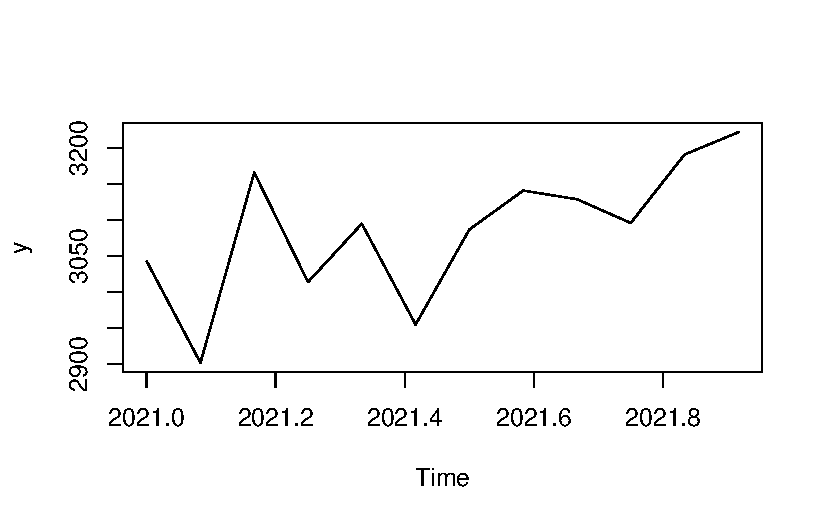
\includegraphics{intro_files/figure-pdf/unnamed-chunk-2-1.pdf}

}

\end{figure}

No gráfico acima, a parte decimal no eixo \(x\) representa a fração do
tempo entre de um ano (começando em 0 e acumulando 1/12 para cada mês
subsequente).

Também podemos customizar o gráfico.

\begin{Shaded}
\begin{Highlighting}[]
\FunctionTok{plot}\NormalTok{(y, }\AttributeTok{ylab =} \StringTok{\textquotesingle{}No. nascidos vivos mensal\textquotesingle{}}\NormalTok{, }\AttributeTok{lwd =} \DecValTok{2}\NormalTok{, }\AttributeTok{col =} \StringTok{\textquotesingle{}seagreen\textquotesingle{}}\NormalTok{)}
\end{Highlighting}
\end{Shaded}

\begin{figure}[H]

{\centering \includegraphics{intro_files/figure-pdf/unnamed-chunk-3-1.pdf}

}

\end{figure}

A função \texttt{window} seleciona um subconjunto da série temporal.
Abaixo selecionamos apenas os nascimentos entre Junho e Agosto e
marcamos estes valores no gráfico.

\begin{Shaded}
\begin{Highlighting}[]
\NormalTok{z }\OtherTok{\textless{}{-}} \FunctionTok{window}\NormalTok{(y, }\AttributeTok{start=}\FunctionTok{c}\NormalTok{(}\DecValTok{2021}\NormalTok{,}\DecValTok{6}\NormalTok{), }\AttributeTok{end =} \FunctionTok{c}\NormalTok{(}\DecValTok{2021}\NormalTok{,}\DecValTok{8}\NormalTok{))}

\FunctionTok{plot}\NormalTok{(y, }\AttributeTok{ylab =} \StringTok{\textquotesingle{}No. nascidos vivos mensal\textquotesingle{}}\NormalTok{, }\AttributeTok{lwd =} \DecValTok{2}\NormalTok{, }\AttributeTok{col =} \StringTok{\textquotesingle{}seagreen\textquotesingle{}}\NormalTok{)}
\FunctionTok{lines}\NormalTok{(z, }\AttributeTok{col =} \StringTok{\textquotesingle{}brown\textquotesingle{}}\NormalTok{, }\AttributeTok{lwd=} \DecValTok{2}\NormalTok{)}
\end{Highlighting}
\end{Shaded}

\begin{figure}[H]

{\centering 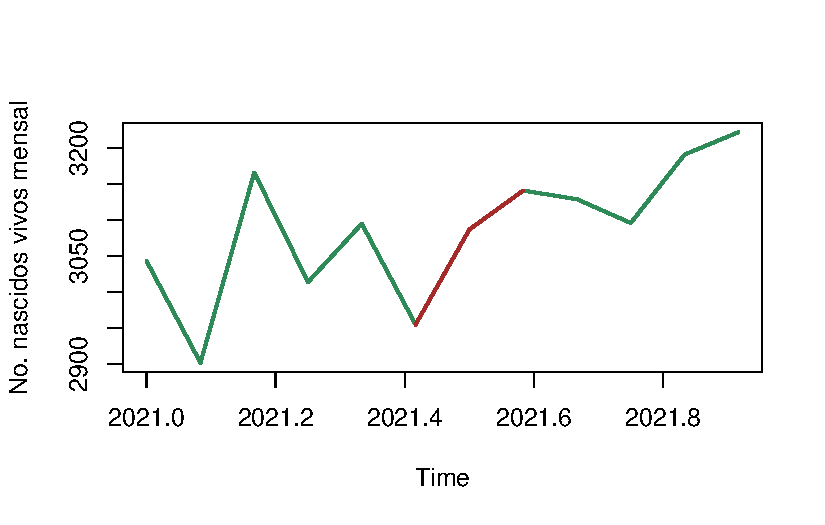
\includegraphics{intro_files/figure-pdf/unnamed-chunk-4-1.pdf}

}

\end{figure}

Exercício 1 Considere o total mensal de nascidos vivos na cidade de
Manaus entre 2019 e 2020:

\begin{longtable}[]{@{}lll@{}}
\toprule\noalign{}
Ano & Mês & No.~nascidos vivos \\
\midrule\noalign{}
\endhead
\bottomrule\noalign{}
\endlastfoot
2019 & 1 & 3.199 \\
& 2 & 2.963 \\
& 3 & 3.146 \\
& 4 & 2.966 \\
& 5 & 3.074 \\
& 6 & 2.919 \\
& 7 & 3.129 \\
& 8 & 3.230 \\
& 9 & 3.456 \\
& 10 & 3.486 \\
& 11 & 3.220 \\
& 12 & 3.151 \\
2020 & 1 & 3.185 \\
& 2 & 3.131 \\
& 3 & 3.256 \\
& 4 & 3.008 \\
& 5 & 3.080 \\
& 6 & 2.919 \\
& 7 & 3.208 \\
& 8 & 3.126 \\
& 9 & 3.126 \\
& 10 & 3.210 \\
& 11 & 2.957 \\
& 12 & 3.068 \\
\end{longtable}

\begin{enumerate}
\def\labelenumi{\arabic{enumi}.}
\item
  Construa um único vetor com os três anos apresentados
\item
  A partir do vetor criado, construa um objeto do tipo \texttt{ts}
\item
  Faça um gráfico da série.
\item
  Crie um janela para ver apenas o ano de 2020.
\item
  Represente a janela acima no gráfico anterior.
\end{enumerate}

\hypertarget{o-pacote-data.table}{%
\section{\texorpdfstring{O pacote
\texttt{data.table}}{O pacote data.table}}\label{o-pacote-data.table}}

Assim como números e textos possuem classes específicas, as datas no
ambiente \texttt{R} também possuem sua \texttt{Date}.

\begin{Shaded}
\begin{Highlighting}[]
\CommentTok{\# 3 de agosto de 1998 (formato americano)}
\NormalTok{x }\OtherTok{\textless{}{-}} \StringTok{\textquotesingle{}1998/8/3\textquotesingle{}}
\FunctionTok{as.Date}\NormalTok{(x)}
\end{Highlighting}
\end{Shaded}

\begin{verbatim}
[1] "1998-08-03"
\end{verbatim}

Para que o \texttt{R} entenda uma data no formato nacional, é necessário
mudar o formato:

\begin{Shaded}
\begin{Highlighting}[]
\CommentTok{\# 3 de agosto de 1998 (formato nacional)}
\NormalTok{x }\OtherTok{\textless{}{-}} \StringTok{\textquotesingle{}3/8/1998\textquotesingle{}}
\FunctionTok{as.Date}\NormalTok{(x, }\AttributeTok{format =} \StringTok{\textquotesingle{}\%d/\%m/\%Y\textquotesingle{}}\NormalTok{)}
\end{Highlighting}
\end{Shaded}

\begin{verbatim}
[1] "1998-08-03"
\end{verbatim}

Lidamos com datas quando temos uma fonte de dados bruta, mas em geral
nosso objetivo é determinar a quantidade de eventos dentro de dias,
semanas, meses ou anos. O pacote \texttt{data.table} permite lidar com
esse problema de modo rápido. Podemos criar um objeto deste tipo
utilizando a função \texttt{fread}. A seguir, vamos baixar uma base de
dados de acidentes com aeronaves, mantida pela Força Aérea Brasileira e
transformar a data de formato nacional para a classe \texttt{Date}.

\begin{Shaded}
\begin{Highlighting}[]
\FunctionTok{library}\NormalTok{(data.table)}
\NormalTok{url }\OtherTok{\textless{}{-}} \StringTok{\textquotesingle{}https://drive.google.com/uc?authuser=0\&id=1iYrnwXgmLK07x8b330aD73scOVruZEuz\&export=download\textquotesingle{}}

\NormalTok{aereo }\OtherTok{\textless{}{-}}  \FunctionTok{fread}\NormalTok{(url, }\AttributeTok{encoding =} \StringTok{\textquotesingle{}Latin{-}1\textquotesingle{}}\NormalTok{)}
\NormalTok{aereo}\SpecialCharTok{$}\NormalTok{ocorrencia\_dia }\OtherTok{\textless{}{-}} \FunctionTok{as.Date}\NormalTok{(aereo}\SpecialCharTok{$}\NormalTok{ocorrencia\_dia, }\StringTok{\textquotesingle{}\%d/\%m/\%Y\textquotesingle{}}\NormalTok{)}
\end{Highlighting}
\end{Shaded}

Um objeto do tipo \texttt{data.table} permite uma série de consultas. Em
geral, pode-se fazer \texttt{aereo{[}a,b,c{]}}, onde \texttt{a} é uma
consulta/função nas linhas, \texttt{b} nas colunas e \texttt{c} é um
agrupador. Uma excelente introdução pode ser vista em
\href{https://cran.r-project.org/web/packages/data.table/vignettes/datatable-intro.html}{Introduction
to data.table}.

Abaixo, selecionamos apenas a coluna de interesse.

\begin{Shaded}
\begin{Highlighting}[]
\NormalTok{fab\_dia }\OtherTok{\textless{}{-}}\NormalTok{ aereo[,}\StringTok{\textquotesingle{}ocorrencia\_dia\textquotesingle{}}\NormalTok{,]}
\FunctionTok{head}\NormalTok{(fab\_dia)}
\end{Highlighting}
\end{Shaded}

\begin{verbatim}
   ocorrencia_dia
1:     2023-04-05
2:     2023-06-24
3:     2023-06-27
4:     2023-06-30
5:     2023-06-25
6:     2023-06-23
\end{verbatim}

Ao utilizar o operador \texttt{.N} em \texttt{{[},.N,c{]}}, é retornado
o número de linhas que possuem o agrupamento em \texttt{c}. Vamos
agrupar as datas do nosso banco por ano.

\begin{Shaded}
\begin{Highlighting}[]
\NormalTok{fab\_ano }\OtherTok{\textless{}{-}}\NormalTok{ fab\_dia[, .N, by}\OtherTok{=}\NormalTok{.(}\FunctionTok{year}\NormalTok{(ocorrencia\_dia))]}
\NormalTok{fab\_ano }\OtherTok{\textless{}{-}}\NormalTok{fab\_ano[ }\FunctionTok{order}\NormalTok{(year) ]}
\FunctionTok{head}\NormalTok{(fab\_ano)}
\end{Highlighting}
\end{Shaded}

\begin{verbatim}
   year   N
1: 2013 654
2: 2014 569
3: 2015 471
4: 2016 403
5: 2017 432
6: 2018 444
\end{verbatim}

Agora, podemos fazer o gráfico da série

\begin{Shaded}
\begin{Highlighting}[]
\NormalTok{fab\_ano }\OtherTok{\textless{}{-}} \FunctionTok{ts}\NormalTok{( fab\_ano, }\AttributeTok{start =} \DecValTok{2013}\NormalTok{)}
\FunctionTok{plot}\NormalTok{(fab\_ano[,}\DecValTok{2}\NormalTok{], }\AttributeTok{lwd =} \DecValTok{2}\NormalTok{, }\AttributeTok{ylab =} \StringTok{\textquotesingle{}No. acidentes/ano\textquotesingle{}}\NormalTok{, }\AttributeTok{xlab =} \StringTok{\textquotesingle{}Ano\textquotesingle{}}\NormalTok{)}
\end{Highlighting}
\end{Shaded}

\begin{figure}[H]

{\centering \includegraphics{intro_files/figure-pdf/unnamed-chunk-10-1.pdf}

}

\end{figure}

Também podemos fazer uma série mensal:

\begin{Shaded}
\begin{Highlighting}[]
\NormalTok{fab\_mes }\OtherTok{\textless{}{-}}\NormalTok{ fab\_dia[, .N, by}\OtherTok{=}\NormalTok{.(}\FunctionTok{year}\NormalTok{(ocorrencia\_dia), }\FunctionTok{month}\NormalTok{(ocorrencia\_dia))]}

\NormalTok{fab\_mes }\OtherTok{\textless{}{-}}\NormalTok{fab\_mes[ }\FunctionTok{order}\NormalTok{(year, month ) ]}
\FunctionTok{head}\NormalTok{(fab\_mes)}
\end{Highlighting}
\end{Shaded}

\begin{verbatim}
   year month  N
1: 2013     1 58
2: 2013     2 60
3: 2013     3 64
4: 2013     4 60
5: 2013     5 60
6: 2013     6 49
\end{verbatim}

O gráfico dessa nova série é:

\begin{Shaded}
\begin{Highlighting}[]
\NormalTok{fab\_mes }\OtherTok{\textless{}{-}} \FunctionTok{ts}\NormalTok{( fab\_mes[,}\DecValTok{3}\NormalTok{], }\AttributeTok{start =} \FunctionTok{c}\NormalTok{(}\DecValTok{2013}\NormalTok{, }\DecValTok{1}\NormalTok{), }\AttributeTok{frequency =} \DecValTok{12}\NormalTok{)}
\FunctionTok{plot}\NormalTok{(fab\_mes, }\AttributeTok{lwd =} \DecValTok{2}\NormalTok{, }\AttributeTok{ylab =} \StringTok{\textquotesingle{}No. acidentes/mês\textquotesingle{}}\NormalTok{, }\AttributeTok{xlab =} \StringTok{\textquotesingle{}Ano\textquotesingle{}}\NormalTok{)}
\end{Highlighting}
\end{Shaded}

\begin{figure}[H]

{\centering 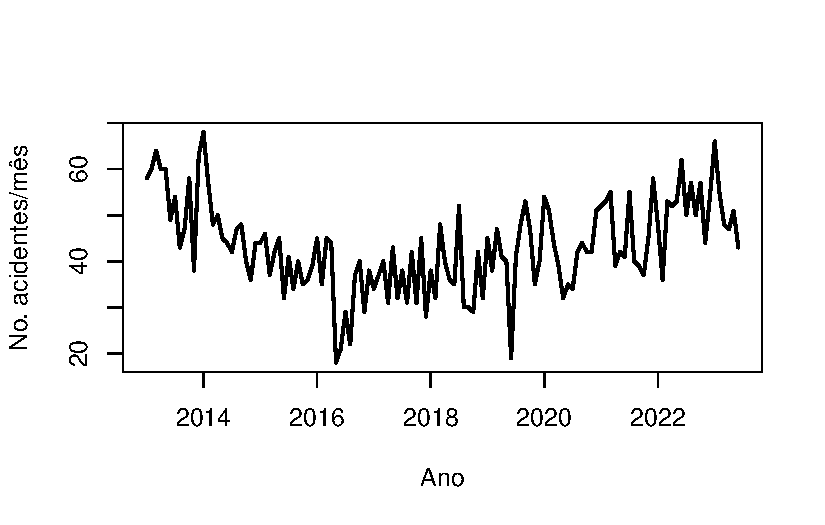
\includegraphics{intro_files/figure-pdf/unnamed-chunk-12-1.pdf}

}

\end{figure}

Exercício 1

A série abaixo contém a data dos óbitos maternos no Brasil a partir de
2010.

\begin{Shaded}
\begin{Highlighting}[]
\NormalTok{url }\OtherTok{\textless{}{-}} \StringTok{\textquotesingle{}https://drive.google.com/uc?authuser=0\&id=1tYFFT9L2iopKmBDUI3P8qNIRaOnMYj7d\&export=download\textquotesingle{}}
\end{Highlighting}
\end{Shaded}

Crie uma série temporal com o número de óbitos mensal e faça um gráfico.
Crie uma janela para colocar no gráfico o período da pandemia de
COVID-19.

\bookmarksetup{startatroot}

\hypertarget{tipos-de-sinal}{%
\chapter{Tipos de sinal}\label{tipos-de-sinal}}

Em geral, a série temporal possui componentes de dois tipos: sinal e
ruído. O primeiro é uma função do tempo geralmente relacionado com a
média da série, enquanto que o segundo está relacionado com a variância.
Podemos assumir que essa relação é aditiva:

\[X_t=\hbox{sinal}(t)+\varepsilon_t\] onde \(\varepsilon_t\) é o ruído.
Em alguns casos essa relação é multiplicativa, ou seja,

\[X_t=\exp\{\hbox{sinal}(t)+\varepsilon_t\},\] e, nesses casos,
aplicamos o logaritmo na série para que as componentes se tornem
aditivas.

Os sinais mais importantes são:

\begin{itemize}
\item
  Tendência: um comportamento de subida ou descida que pode ser
  observado no médio/longo prazo
\item
  Sazonalidade: são componentes que surgem sistematicamente ao longo do
  tempo, como por exemplo: flutuações de temperatura entre estações,
  início e fim do semestre letivo, Natal, dias úteis, feriados
  flutuantes como a Páscoa e o Carnaval.
\end{itemize}

O ruídos mais importantes são:

\begin{itemize}
\item
  Branco: possuem variância constante e não correlacionados.
\item
  Média móvel de ordem \(q\): possuem variância constante e são
  correlacionados com até \(q\) ruídos anteriores.
\end{itemize}

A série a seguir representa o número de vendas de passagens aéreas nos
EUA. Note o comportamento da tendência e da sazonalidade.

\begin{Shaded}
\begin{Highlighting}[]
\FunctionTok{plot}\NormalTok{(AirPassengers)}
\end{Highlighting}
\end{Shaded}

\begin{figure}[H]

{\centering 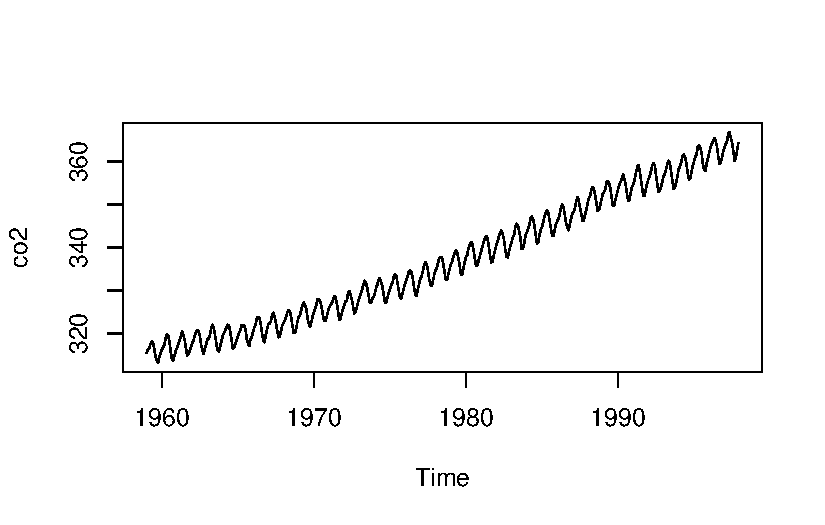
\includegraphics{sinal_files/figure-pdf/unnamed-chunk-1-1.pdf}

}

\end{figure}

\bookmarksetup{startatroot}

\hypertarget{a-funuxe7uxe3o-de-autocorrelauxe7uxe3o}{%
\chapter{A função de
autocorrelação}\label{a-funuxe7uxe3o-de-autocorrelauxe7uxe3o}}

Considere inicialmente uma amostra aleatória \(X_1,\ldots,X_n\) (ou
seja, todas as variáveis são independentes e possuem a mesma
distribuição). Sejam \[A_h=\{X_1,\ldots,X_{n-h}\}\] e
\[B_h=\{X_h,\ldots,X_n\}.\] Então, a correlação entre \(A_h\) e \(B_h\)
é nula.

Deste modo, um meio de verificar se a coleção observada é uma série
temporal é observar a correlação amostral entre
\[a_h=\{x_1,\ldots,x_{n-h}\}\] e \[b_h=\{x_h,\ldots,x_n\},\] para
diferentes valores de \(h\).

A função \(r(h)\) que representa a correlação amostral entre \(a_h\) e
\(b_h\) é denominada \textbf{autocorrelação}. O valor \(h\) é denominado
\textbf{defasagem} (do inglês, \emph{lag}).

Propriedades

\begin{itemize}
\item
  \(r(0)=1\)
\item
  \(-1\leq r(h) \leq 1\)
\end{itemize}

Correlograma O gráfico \((h,r(h))\) é denominado correlograma, ou
gráfico da função de autocorrelação.

\hypertarget{o-correlograma-de-uma-amostra-aleatuxf3ria}{%
\section{O correlograma de uma amostra
aleatória}\label{o-correlograma-de-uma-amostra-aleatuxf3ria}}

Quando a amostra é aleatória, a função de autocorrelação é nula para
qualquer defasagem diferente de 0. Deste modo, o correlograma deve
apresentar valores próximos de zero.

Para entender o que próximo de zero significa, o limites do intervalo de
confiança para o coeficiente de correlação sobre a hipótese de que esta
é nula são colocados no gráfico.

Abaixo ilustramos um correlograma para uma amostra de variáveis
aleatórias independentes com distribuição normal padrão.

\begin{Shaded}
\begin{Highlighting}[]
\NormalTok{x }\OtherTok{\textless{}{-}} \FunctionTok{rnorm}\NormalTok{(}\DecValTok{120}\NormalTok{)}

\CommentTok{\# correlograma}
\FunctionTok{acf}\NormalTok{(x)}
\end{Highlighting}
\end{Shaded}

\begin{figure}[H]

{\centering \includegraphics{acf_files/figure-pdf/unnamed-chunk-1-1.pdf}

}

\end{figure}

\begin{Shaded}
\begin{Highlighting}[]
\CommentTok{\# o mesmo correlograma com uma defasagem maior}
\FunctionTok{acf}\NormalTok{(x, }\AttributeTok{lag =} \DecValTok{50}\NormalTok{)}
\end{Highlighting}
\end{Shaded}

\begin{figure}[H]

{\centering 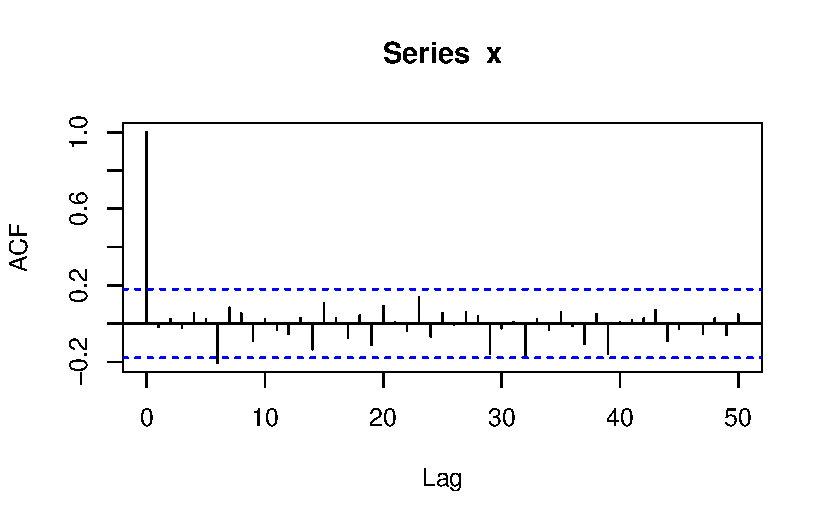
\includegraphics{acf_files/figure-pdf/unnamed-chunk-1-2.pdf}

}

\end{figure}

\hypertarget{o-correlograma-com-a-componente-de-tenduxeancia}{%
\section{O correlograma com a componente de
tendência}\label{o-correlograma-com-a-componente-de-tenduxeancia}}

Quando uma série exibe tendência, o correlograma exibe um descaimento
lento e persistente.

Considere, por exemplo, a série

\[x_t= t + \varepsilon_t,\] onde
\(\varepsilon_t\sim\hbox{Normal}(0,5^2)\). Abaixo simulamos essa série e
apresentamos o respectivo correlograma

\begin{Shaded}
\begin{Highlighting}[]
\NormalTok{x }\OtherTok{\textless{}{-}} \FunctionTok{rnorm}\NormalTok{(}\DecValTok{100}\NormalTok{, }\DecValTok{1}\SpecialCharTok{:}\DecValTok{100}\NormalTok{, }\DecValTok{5}\NormalTok{)}

\NormalTok{oo }\OtherTok{\textless{}{-}} \FunctionTok{par}\NormalTok{( }\AttributeTok{mfrow=}\FunctionTok{c}\NormalTok{(}\DecValTok{1}\NormalTok{,}\DecValTok{2}\NormalTok{))}
\FunctionTok{ts.plot}\NormalTok{(x)}
\FunctionTok{acf}\NormalTok{(x, }\AttributeTok{lag =} \DecValTok{50}\NormalTok{)}
\end{Highlighting}
\end{Shaded}

\begin{figure}[H]

{\centering \includegraphics{acf_files/figure-pdf/unnamed-chunk-2-1.pdf}

}

\end{figure}

\begin{Shaded}
\begin{Highlighting}[]
\FunctionTok{par}\NormalTok{(oo)}
\end{Highlighting}
\end{Shaded}

Observe as similaridades do correlograma acima com o observado para a
série de acidentes aéreos mensais vista anteriormente.

\begin{Shaded}
\begin{Highlighting}[]
\NormalTok{oo }\OtherTok{\textless{}{-}} \FunctionTok{par}\NormalTok{( }\AttributeTok{mfrow=}\FunctionTok{c}\NormalTok{(}\DecValTok{1}\NormalTok{,}\DecValTok{2}\NormalTok{))}
\FunctionTok{ts.plot}\NormalTok{( fab\_mes , }\AttributeTok{ylab =} \StringTok{\textquotesingle{}No. acidentes aéreos mensal\textquotesingle{}}\NormalTok{ )}
\FunctionTok{acf}\NormalTok{(fab\_mes , }\AttributeTok{lag =} \DecValTok{50}\NormalTok{,  }\AttributeTok{main =}\StringTok{\textquotesingle{}correlograma\textquotesingle{}}\NormalTok{)}
\end{Highlighting}
\end{Shaded}

\begin{figure}[H]

{\centering 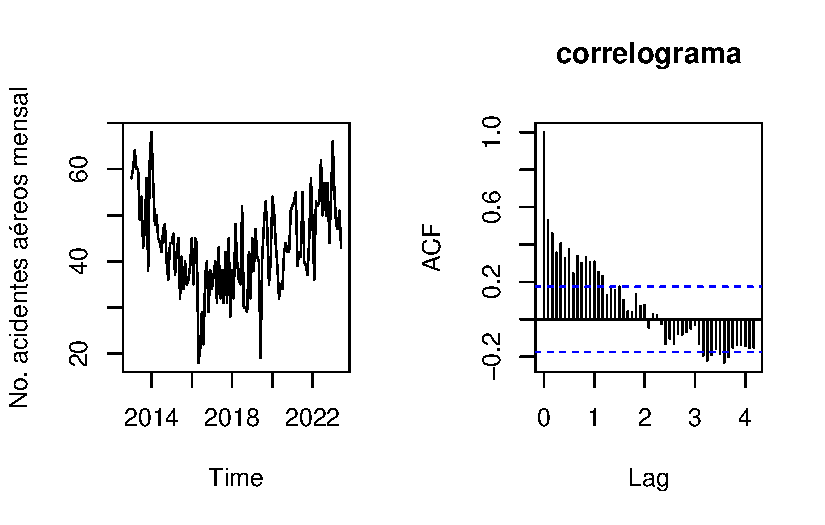
\includegraphics{acf_files/figure-pdf/unnamed-chunk-4-1.pdf}

}

\end{figure}

\begin{Shaded}
\begin{Highlighting}[]
\FunctionTok{par}\NormalTok{(oo)}
\end{Highlighting}
\end{Shaded}

\hypertarget{o-correlograma-com-a-componente-de-sazonalidade---sinal-harmuxf4nico}{%
\section{O correlograma com a componente de sazonalidade - sinal
harmônico}\label{o-correlograma-com-a-componente-de-sazonalidade---sinal-harmuxf4nico}}

O sinal sazonal é caracterizado por um comportamento periódico. Existem
dois comportamentos sazonais típicos. O primeiro é baseado na função
harmônica:

\[\hbox{sinal}(t)=A\cos\left(\frac{2\pi}{p}t + \phi\right)\] Neste tipo
de sinal, há um comportamento em forma de onda já estabelecido. Eis
algumas informações importantes:

\begin{itemize}
\item
  O valor \(p\), denominado período, equivale ao tempo que demora para o
  padrão se repetir.
\item
  \(A\) é denominado amplitude e representa o maior/menor valor que este
  sinal pode aingir.
\item
  Por último, \(\phi\) é denominado fase, e serve basicamente para
  deslocar a onda.
\end{itemize}

Abaixo seguem alguns exemplos de harmônicos, todos com período 12:

\begin{Shaded}
\begin{Highlighting}[]
\NormalTok{oo }\OtherTok{\textless{}{-}} \FunctionTok{par}\NormalTok{( }\AttributeTok{cex =} \FloatTok{1.3}\NormalTok{)}
\FunctionTok{curve}\NormalTok{( }\FunctionTok{cos}\NormalTok{( x}\SpecialCharTok{*} \DecValTok{2}\SpecialCharTok{*}\NormalTok{pi}\SpecialCharTok{/}\DecValTok{12}\NormalTok{), }\DecValTok{0}\NormalTok{,}\DecValTok{24}\NormalTok{, }\AttributeTok{lwd =} \DecValTok{2}\NormalTok{, }\AttributeTok{ylab =} \FunctionTok{expression}\NormalTok{( }\FunctionTok{cos}\NormalTok{( }\DecValTok{2}\SpecialCharTok{*}\NormalTok{pi}\SpecialCharTok{*}\NormalTok{t}\SpecialCharTok{/}\DecValTok{12}\NormalTok{ )))}
\FunctionTok{abline}\NormalTok{(}\AttributeTok{h =} \DecValTok{0}\NormalTok{, }\AttributeTok{lty =} \DecValTok{2}\NormalTok{ )}
\FunctionTok{abline}\NormalTok{(}\AttributeTok{v=}\DecValTok{12}\NormalTok{, }\AttributeTok{lty =} \DecValTok{2}\NormalTok{)}
\end{Highlighting}
\end{Shaded}

\begin{figure}[H]

{\centering 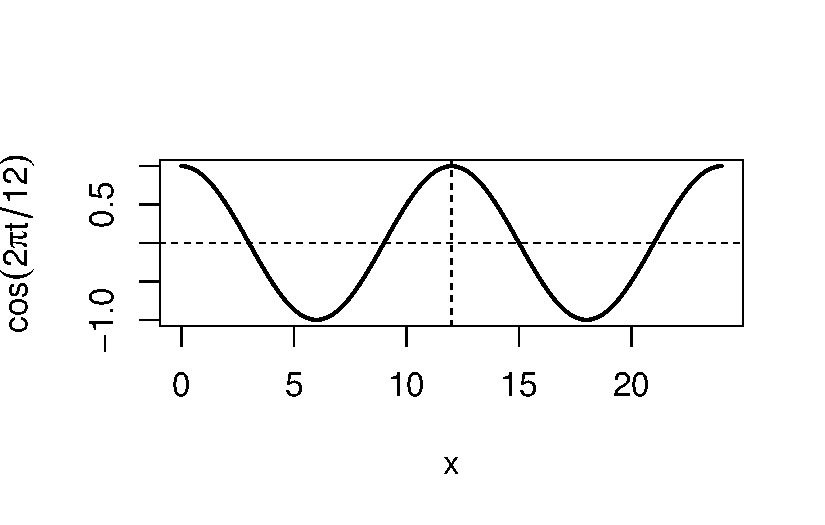
\includegraphics{acf_files/figure-pdf/unnamed-chunk-5-1.pdf}

}

\end{figure}

\begin{Shaded}
\begin{Highlighting}[]
\FunctionTok{curve}\NormalTok{( .}\DecValTok{5}\SpecialCharTok{*}\FunctionTok{cos}\NormalTok{( x}\SpecialCharTok{*} \DecValTok{2}\SpecialCharTok{*}\NormalTok{pi}\SpecialCharTok{/}\DecValTok{12}\NormalTok{), }\DecValTok{0}\NormalTok{,}\DecValTok{24}\NormalTok{, }\AttributeTok{lwd =} \DecValTok{2}\NormalTok{, }\AttributeTok{ylab =} \FunctionTok{expression}\NormalTok{( .}\DecValTok{5}\SpecialCharTok{*}\FunctionTok{cos}\NormalTok{( }\DecValTok{2}\SpecialCharTok{*}\NormalTok{pi}\SpecialCharTok{*}\NormalTok{t}\SpecialCharTok{/}\DecValTok{12}\NormalTok{ )), }\AttributeTok{ylim =} \FunctionTok{c}\NormalTok{(}\SpecialCharTok{{-}}\DecValTok{1}\NormalTok{,}\DecValTok{1}\NormalTok{))}
\FunctionTok{abline}\NormalTok{(}\AttributeTok{h =} \DecValTok{0}\NormalTok{, }\AttributeTok{lty =} \DecValTok{2}\NormalTok{ )}
\FunctionTok{abline}\NormalTok{(}\AttributeTok{v=}\DecValTok{12}\NormalTok{, }\AttributeTok{lty =} \DecValTok{2}\NormalTok{)}
\end{Highlighting}
\end{Shaded}

\begin{figure}[H]

{\centering \includegraphics{acf_files/figure-pdf/unnamed-chunk-5-2.pdf}

}

\end{figure}

\begin{Shaded}
\begin{Highlighting}[]
\FunctionTok{curve}\NormalTok{( }\FunctionTok{cos}\NormalTok{( x}\SpecialCharTok{*} \DecValTok{2}\SpecialCharTok{*}\NormalTok{pi}\SpecialCharTok{/}\DecValTok{12}\SpecialCharTok{+}\DecValTok{90}\NormalTok{), }\DecValTok{0}\NormalTok{,}\DecValTok{24}\NormalTok{, }\AttributeTok{lwd =} \DecValTok{2}\NormalTok{, }\AttributeTok{ylab =} \FunctionTok{expression}\NormalTok{( }\FunctionTok{cos}\NormalTok{( }\DecValTok{2}\SpecialCharTok{*}\NormalTok{pi}\SpecialCharTok{*}\NormalTok{t}\SpecialCharTok{/}\DecValTok{12} \SpecialCharTok{+}\DecValTok{90}\NormalTok{)), }\AttributeTok{ylim =} \FunctionTok{c}\NormalTok{(}\SpecialCharTok{{-}}\DecValTok{1}\NormalTok{,}\DecValTok{1}\NormalTok{))}
\FunctionTok{abline}\NormalTok{(}\AttributeTok{h =} \DecValTok{0}\NormalTok{, }\AttributeTok{lty =} \DecValTok{2}\NormalTok{ )}
\FunctionTok{abline}\NormalTok{(}\AttributeTok{v=}\DecValTok{12}\NormalTok{, }\AttributeTok{lty =} \DecValTok{2}\NormalTok{)}
\end{Highlighting}
\end{Shaded}

\begin{figure}[H]

{\centering 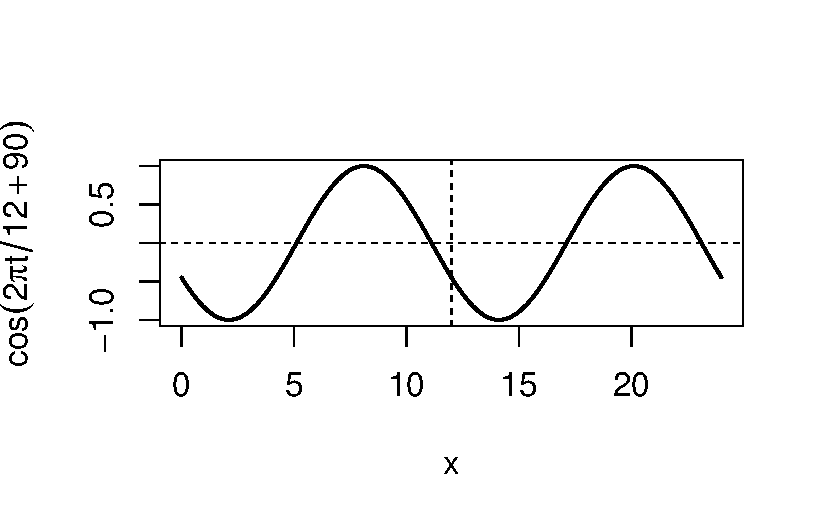
\includegraphics{acf_files/figure-pdf/unnamed-chunk-5-3.pdf}

}

\end{figure}

Abaixo simulamos uma série temporal com um sinal do tipo harmônico.
Observe que o comportamento em forma de onda é aparente na função de
autocorrelação.

\begin{Shaded}
\begin{Highlighting}[]
\NormalTok{x }\OtherTok{\textless{}{-}} \FunctionTok{cos}\NormalTok{( }\DecValTok{2}\SpecialCharTok{*}\NormalTok{pi}\SpecialCharTok{/}\DecValTok{12} \SpecialCharTok{*} \DecValTok{1}\SpecialCharTok{:}\DecValTok{100}\NormalTok{) }\SpecialCharTok{+} \FunctionTok{rnorm}\NormalTok{(}\DecValTok{100}\NormalTok{,}\DecValTok{0}\NormalTok{,.}\DecValTok{1}\NormalTok{)}

\NormalTok{oo }\OtherTok{\textless{}{-}} \FunctionTok{par}\NormalTok{( }\AttributeTok{mfrow =} \FunctionTok{c}\NormalTok{(}\DecValTok{1}\NormalTok{,}\DecValTok{2}\NormalTok{))}
\FunctionTok{ts.plot}\NormalTok{(x)}
\FunctionTok{acf}\NormalTok{(x)}
\end{Highlighting}
\end{Shaded}

\begin{figure}[H]

{\centering 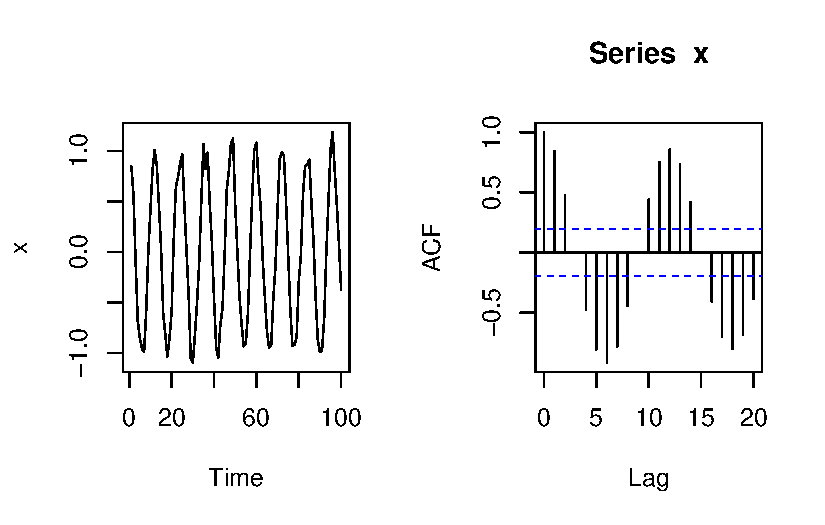
\includegraphics{acf_files/figure-pdf/unnamed-chunk-6-1.pdf}

}

\end{figure}

\begin{Shaded}
\begin{Highlighting}[]
\FunctionTok{par}\NormalTok{(oo)}
\end{Highlighting}
\end{Shaded}

Abaixo, apresentamos a temperatura mensal observada no Castelo de
Nottingham, entre 1920-1939. Compare os resultados com os gráficos
acima.

\begin{Shaded}
\begin{Highlighting}[]
\NormalTok{oo }\OtherTok{\textless{}{-}} \FunctionTok{par}\NormalTok{( }\AttributeTok{mfrow =} \FunctionTok{c}\NormalTok{(}\DecValTok{1}\NormalTok{,}\DecValTok{2}\NormalTok{))}
  \FunctionTok{plot}\NormalTok{(nottem)}
  \FunctionTok{acf}\NormalTok{(nottem)}
\end{Highlighting}
\end{Shaded}

\begin{figure}[H]

{\centering 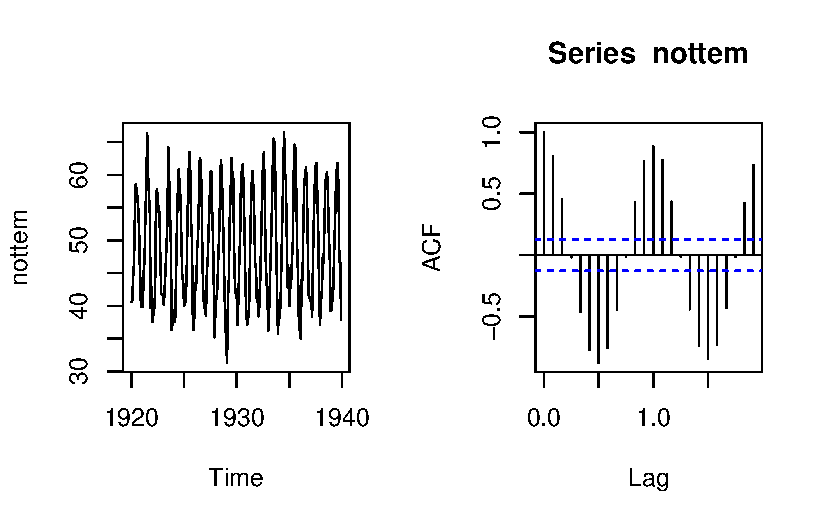
\includegraphics{acf_files/figure-pdf/unnamed-chunk-7-1.pdf}

}

\end{figure}

\begin{Shaded}
\begin{Highlighting}[]
\FunctionTok{par}\NormalTok{(oo)  }
\end{Highlighting}
\end{Shaded}

\hypertarget{o-correlograma-com-a-componente-de-sazonalidade---sinal-autorregressivo}{%
\section{O correlograma com a componente de sazonalidade - sinal
autorregressivo}\label{o-correlograma-com-a-componente-de-sazonalidade---sinal-autorregressivo}}

Nesse tipo de sazonalidade, ainda há um período \(p\), mas não há um
sinal harmônico. O valor da série no tempo \(t\) é baseado no valor
observado no tempo \(t-p\).

Quando a sazonalidade possue essa característica, há uma autocorrelação
marcante nos múltiplos de \(p\). Observe a série simulada abaixo, com um
período \(p=12\)

\begin{Shaded}
\begin{Highlighting}[]
\FunctionTok{set.seed}\NormalTok{(}\DecValTok{123}\NormalTok{)}
\NormalTok{oo }\OtherTok{\textless{}{-}} \FunctionTok{par}\NormalTok{( }\AttributeTok{mfrow =} \FunctionTok{c}\NormalTok{(}\DecValTok{1}\NormalTok{,}\DecValTok{2}\NormalTok{))}
\NormalTok{x }\OtherTok{\textless{}{-}} \FunctionTok{rnorm}\NormalTok{(}\DecValTok{12}\NormalTok{,}\DecValTok{0}\NormalTok{,.}\DecValTok{1}\NormalTok{)}
\ControlFlowTok{for}\NormalTok{(i }\ControlFlowTok{in} \DecValTok{13}\SpecialCharTok{:}\DecValTok{100}\NormalTok{) x[i] }\OtherTok{\textless{}{-}}\NormalTok{ .}\DecValTok{6}\SpecialCharTok{*}\NormalTok{x[i}\DecValTok{{-}12}\NormalTok{] }\SpecialCharTok{+} \FunctionTok{rnorm}\NormalTok{(}\DecValTok{1}\NormalTok{,}\DecValTok{0}\NormalTok{,.}\DecValTok{05}\NormalTok{)}
\FunctionTok{ts.plot}\NormalTok{(x)}
\FunctionTok{acf}\NormalTok{(x, }\AttributeTok{lag =} \DecValTok{50}\NormalTok{)}
\end{Highlighting}
\end{Shaded}

\begin{figure}[H]

{\centering \includegraphics{acf_files/figure-pdf/unnamed-chunk-8-1.pdf}

}

\end{figure}

\begin{Shaded}
\begin{Highlighting}[]
\FunctionTok{par}\NormalTok{(oo)}
\end{Highlighting}
\end{Shaded}

\hypertarget{exercuxedcios}{%
\section{Exercícios}\label{exercuxedcios}}

Exercício 1 Estude o comportamento da série \texttt{ldeaths}, que conta
o número mensal de óbitos por doenças pulmonares no Reino Unido.

Exercício 2 Estude o comportamento da série do número de óbitos maternos
mensais.

Exercício 3 Em 2017, um epidemiologista estava interessado na série de
suicídios no Mato Grosso do Sul. O banco de dados utilizado é dado a
seguir. Construa uma série mensal e estude seu comportamento

\begin{Shaded}
\begin{Highlighting}[]
\NormalTok{url }\OtherTok{\textless{}{-}} \StringTok{\textquotesingle{}https://drive.google.com/uc?authuser=0\&id=1DMSgrQDl0636Lw0Y0MYJHJrgw\_2uXntM\&export=download\textquotesingle{}}
\end{Highlighting}
\end{Shaded}

\bookmarksetup{startatroot}

\hypertarget{mais-ferramentas-exploratuxf3rias}{%
\chapter{Mais ferramentas
exploratórias}\label{mais-ferramentas-exploratuxf3rias}}

\hypertarget{estudo-da-tenduxeancia-utilizando-o-loess}{%
\section{\texorpdfstring{Estudo da tendência utilizando o
\texttt{loess}}{Estudo da tendência utilizando o loess}}\label{estudo-da-tenduxeancia-utilizando-o-loess}}

\emph{Loes} é um modelo de regressão não linear não paramétrico. Abaixo
mostramos como utilizá-lo considerando um banco de dados com diversas
marcas de veículos e a relação entre a variável milhas por galão (mpg) e
deslocamento (disp)

\begin{Shaded}
\begin{Highlighting}[]
\FunctionTok{plot}\NormalTok{( mtcars}\SpecialCharTok{$}\NormalTok{disp, mtcars}\SpecialCharTok{$}\NormalTok{mpg )}
\NormalTok{lw }\OtherTok{\textless{}{-}} \FunctionTok{loess}\NormalTok{( mpg }\SpecialCharTok{\textasciitilde{}}\NormalTok{ disp, }\AttributeTok{data =}\NormalTok{ mtcars )}
\FunctionTok{points}\NormalTok{(mtcars}\SpecialCharTok{$}\NormalTok{disp, lw}\SpecialCharTok{$}\NormalTok{fitted, }\AttributeTok{col =} \StringTok{\textquotesingle{}tomato\textquotesingle{}}\NormalTok{, }\AttributeTok{lwd =} \DecValTok{2}\NormalTok{)}
\FunctionTok{legend}\NormalTok{(}\StringTok{\textquotesingle{}topright\textquotesingle{}}\NormalTok{, }\FunctionTok{c}\NormalTok{(}\StringTok{\textquotesingle{}Observado\textquotesingle{}}\NormalTok{,}\StringTok{\textquotesingle{}Ajustado\textquotesingle{}}\NormalTok{),}\AttributeTok{fill=}\FunctionTok{c}\NormalTok{(}\DecValTok{1}\NormalTok{,}\StringTok{\textquotesingle{}tomato\textquotesingle{}}\NormalTok{), }\AttributeTok{bty=}\StringTok{\textquotesingle{}n\textquotesingle{}}\NormalTok{)}
\end{Highlighting}
\end{Shaded}

\begin{figure}[H]

{\centering 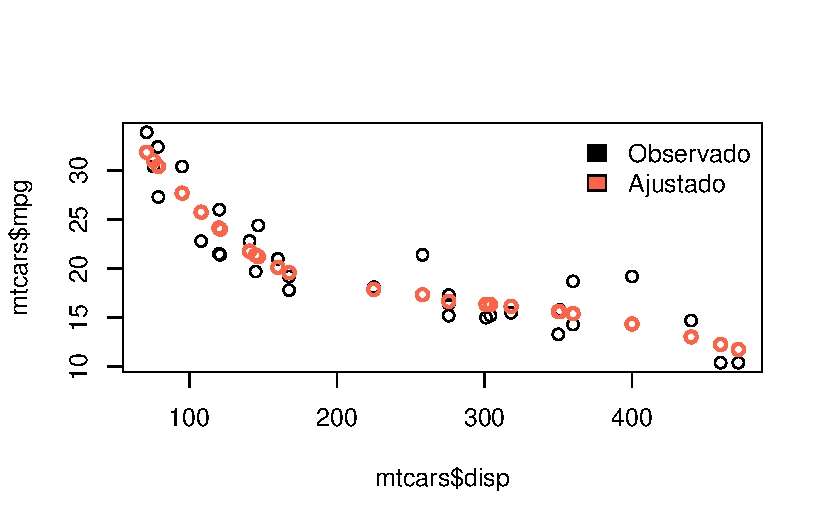
\includegraphics{ferramentas_files/figure-pdf/unnamed-chunk-1-1.pdf}

}

\end{figure}

Podemos estimar a tendência utilizando o loess, imaginando uma regressão
do tipo:

\[E(X_t)=g(t),\] ou seja, utilizando o tempo como regressora. Vamos
ilustrar a ideia utilizando a série de acidentes aéreos mensais da FAB.

\begin{Shaded}
\begin{Highlighting}[]
\CommentTok{\# criando a variável regressora}
\NormalTok{tempo }\OtherTok{\textless{}{-}} \DecValTok{1} \SpecialCharTok{:} \FunctionTok{length}\NormalTok{(fab\_mes)}

\CommentTok{\# aplicando o loess}
\NormalTok{lw }\OtherTok{\textless{}{-}} \FunctionTok{loess}\NormalTok{( fab\_mes }\SpecialCharTok{\textasciitilde{}}\NormalTok{ tempo)}

\CommentTok{\# transformando o valor predito em uma série temporal}

\NormalTok{fit }\OtherTok{\textless{}{-}} \FunctionTok{ts}\NormalTok{(lw}\SpecialCharTok{$}\NormalTok{fitted, }\AttributeTok{start =} \FunctionTok{start}\NormalTok{(fab\_mes), }\AttributeTok{frequency =} \FunctionTok{frequency}\NormalTok{(fab\_mes) )}

\CommentTok{\# gráfico da tendência estimada}

\FunctionTok{ts.plot}\NormalTok{( fab\_mes, }\AttributeTok{ylab =} \StringTok{\textquotesingle{}No. acidentes/mês\textquotesingle{}}\NormalTok{ , }\AttributeTok{lwd =} \DecValTok{2}\NormalTok{)}
\FunctionTok{lines}\NormalTok{(fit, }\AttributeTok{lwd =} \DecValTok{2}\NormalTok{, }\AttributeTok{col =} \StringTok{\textquotesingle{}tomato\textquotesingle{}}\NormalTok{)}
\FunctionTok{legend}\NormalTok{(}\StringTok{\textquotesingle{}bottomright\textquotesingle{}}\NormalTok{, }\FunctionTok{c}\NormalTok{(}\StringTok{\textquotesingle{}Observado\textquotesingle{}}\NormalTok{,}\StringTok{\textquotesingle{}Ajustado\textquotesingle{}}\NormalTok{),}\AttributeTok{fill=}\FunctionTok{c}\NormalTok{(}\DecValTok{1}\NormalTok{,}\StringTok{\textquotesingle{}tomato\textquotesingle{}}\NormalTok{), }\AttributeTok{bty=}\StringTok{\textquotesingle{}n\textquotesingle{}}\NormalTok{)}
\end{Highlighting}
\end{Shaded}

\begin{figure}[H]

{\centering 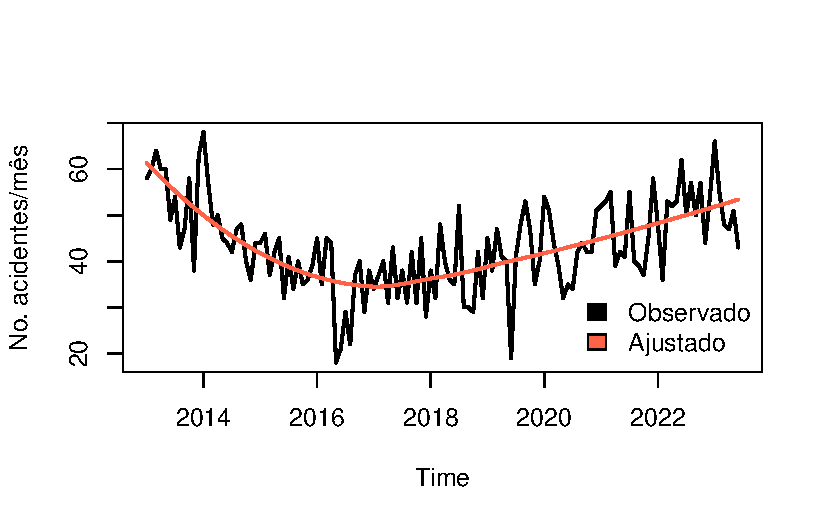
\includegraphics{ferramentas_files/figure-pdf/unnamed-chunk-3-1.pdf}

}

\end{figure}

Acima estimamos a tendência. Denomine este sinal estimado por
\(\hat{g}(t)\). Agora, considere a série

\[y_t=x_t-\hat{g}(t).\] Ao analisar esta série, duas coisas podem
acontecer:

\begin{itemize}
\item
  Vamos encontrar um comportamento semelhante a um ruído (correlograma
  com barras praticamente nulas)
\item
  Vamos encontrar algum outro sinal ainda não ajustado.
\end{itemize}

Os gráficos abaixo mostram que não há mais sinais para procurar

\begin{Shaded}
\begin{Highlighting}[]
\NormalTok{yt }\OtherTok{\textless{}{-}}\NormalTok{ fab\_mes }\SpecialCharTok{{-}}\NormalTok{ fit}

\FunctionTok{ts.plot}\NormalTok{(yt)}
\end{Highlighting}
\end{Shaded}

\begin{figure}[H]

{\centering 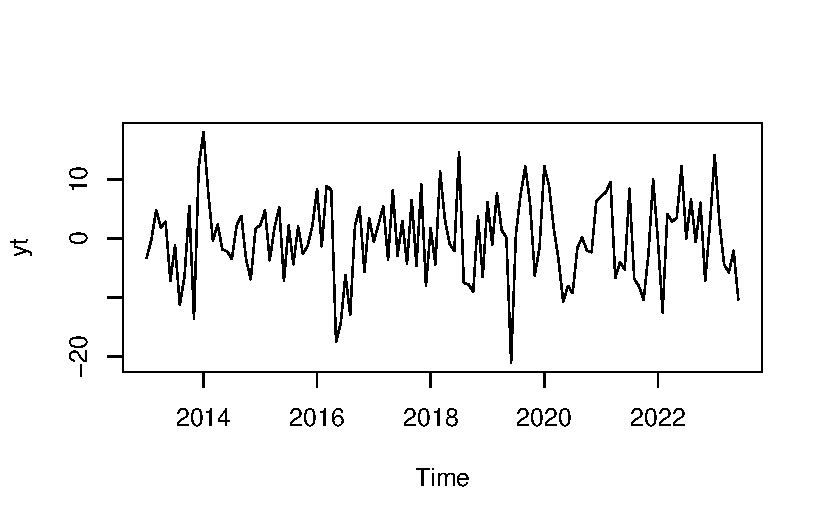
\includegraphics{ferramentas_files/figure-pdf/unnamed-chunk-4-1.pdf}

}

\end{figure}

\begin{Shaded}
\begin{Highlighting}[]
\FunctionTok{acf}\NormalTok{(yt, }\AttributeTok{lag =} \DecValTok{30}\NormalTok{)}
\end{Highlighting}
\end{Shaded}

\begin{figure}[H]

{\centering 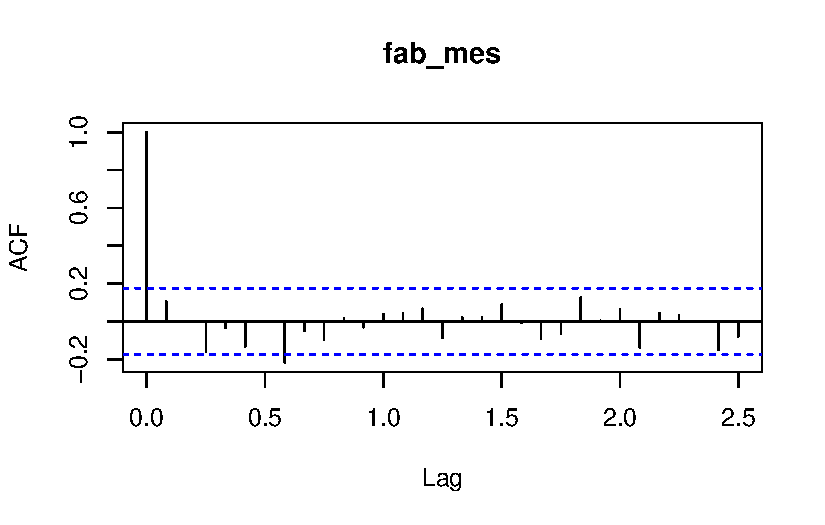
\includegraphics{ferramentas_files/figure-pdf/unnamed-chunk-4-2.pdf}

}

\end{figure}

Portanto, esta série pode ser escrita como

\[x_t = \hbox{tendência}_t+\varepsilon_t,\] onde \(\varepsilon_t\) é um
ruído branco.

Abaixo, vamos analisar a série de taxa de desemprego mensal, entre março
de 2002 e dezembro de 2015.

\begin{Shaded}
\begin{Highlighting}[]
\NormalTok{url }\OtherTok{\textless{}{-}} \StringTok{\textquotesingle{}https://www.dropbox.com/s/rmgymzsic99qawd/desemprego.csv?dl=1\textquotesingle{}}

\NormalTok{banco }\OtherTok{\textless{}{-}} \FunctionTok{fread}\NormalTok{(url)}

\NormalTok{desemprego}\OtherTok{\textless{}{-}} \FunctionTok{ts}\NormalTok{( banco[,}\StringTok{\textquotesingle{}V2\textquotesingle{}}\NormalTok{,], }\AttributeTok{start =} \FunctionTok{c}\NormalTok{(}\DecValTok{2002}\NormalTok{,}\DecValTok{3}\NormalTok{), }\AttributeTok{frequency=}\DecValTok{12}\NormalTok{)}

\FunctionTok{ts.plot}\NormalTok{(desemprego, }\AttributeTok{ylab =} \StringTok{\textquotesingle{}Taxa de desemprego\textquotesingle{}}\NormalTok{)}
\end{Highlighting}
\end{Shaded}

\begin{figure}[H]

{\centering 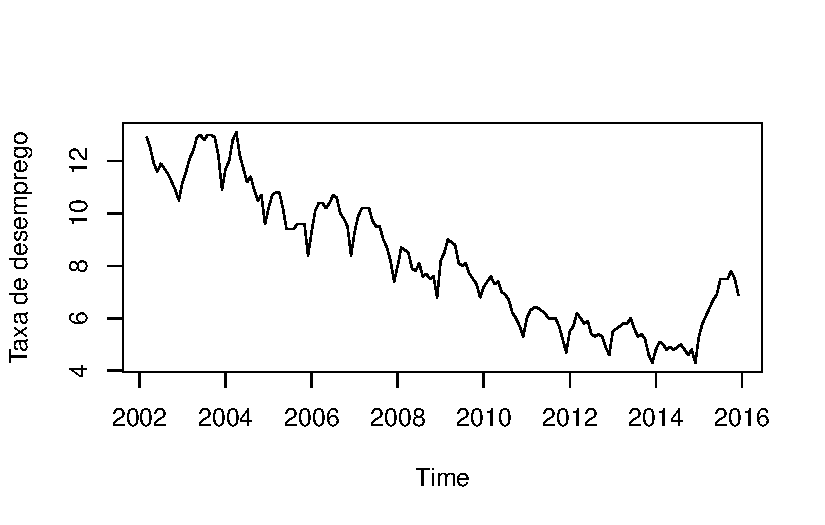
\includegraphics{ferramentas_files/figure-pdf/unnamed-chunk-5-1.pdf}

}

\end{figure}

\begin{Shaded}
\begin{Highlighting}[]
\FunctionTok{acf}\NormalTok{(desemprego, }\AttributeTok{lag =} \DecValTok{30}\NormalTok{)}
\end{Highlighting}
\end{Shaded}

\begin{figure}[H]

{\centering \includegraphics{ferramentas_files/figure-pdf/unnamed-chunk-5-2.pdf}

}

\end{figure}

É possível verificar que há tendência e sazonalidade na série. Vamos
estimar a componente de tendência primeiro.

\begin{Shaded}
\begin{Highlighting}[]
\CommentTok{\# criando a variável regressora}
\NormalTok{tempo }\OtherTok{\textless{}{-}} \DecValTok{1} \SpecialCharTok{:} \FunctionTok{length}\NormalTok{(desemprego)}

\CommentTok{\# aplicando o loess}
\NormalTok{lw }\OtherTok{\textless{}{-}} \FunctionTok{loess}\NormalTok{( desemprego }\SpecialCharTok{\textasciitilde{}}\NormalTok{ tempo)}

\CommentTok{\# transformando o valor predito em uma série temporal}

\NormalTok{fit }\OtherTok{\textless{}{-}} \FunctionTok{ts}\NormalTok{(lw}\SpecialCharTok{$}\NormalTok{fitted, }\AttributeTok{start =} \FunctionTok{start}\NormalTok{(desemprego), }\AttributeTok{frequency =} \FunctionTok{frequency}\NormalTok{(desemprego) )}

\CommentTok{\# gráfico da tendência estimada}

\FunctionTok{ts.plot}\NormalTok{( desemprego, }\AttributeTok{ylab =} \StringTok{\textquotesingle{}Taxa de desemprego\textquotesingle{}}\NormalTok{ , }\AttributeTok{lwd =} \DecValTok{2}\NormalTok{)}
\FunctionTok{lines}\NormalTok{(fit, }\AttributeTok{lwd =} \DecValTok{2}\NormalTok{, }\AttributeTok{col =} \StringTok{\textquotesingle{}tomato\textquotesingle{}}\NormalTok{)}
\FunctionTok{legend}\NormalTok{(}\StringTok{\textquotesingle{}topright\textquotesingle{}}\NormalTok{, }\FunctionTok{c}\NormalTok{(}\StringTok{\textquotesingle{}Observado\textquotesingle{}}\NormalTok{,}\StringTok{\textquotesingle{}Ajustado\textquotesingle{}}\NormalTok{),}\AttributeTok{fill=}\FunctionTok{c}\NormalTok{(}\DecValTok{1}\NormalTok{,}\StringTok{\textquotesingle{}tomato\textquotesingle{}}\NormalTok{), }\AttributeTok{bty=}\StringTok{\textquotesingle{}n\textquotesingle{}}\NormalTok{)}
\end{Highlighting}
\end{Shaded}

\begin{figure}[H]

{\centering 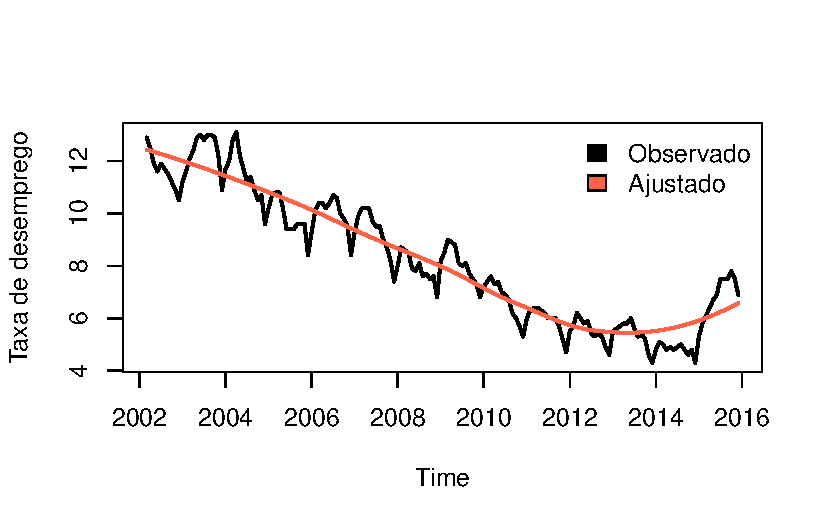
\includegraphics{ferramentas_files/figure-pdf/unnamed-chunk-6-1.pdf}

}

\end{figure}

Vamos eliminar a tendência estiamada e avaliar o restante.

\begin{Shaded}
\begin{Highlighting}[]
\NormalTok{yt }\OtherTok{\textless{}{-}}\NormalTok{ desemprego }\SpecialCharTok{{-}}\NormalTok{ fit}

\FunctionTok{ts.plot}\NormalTok{(yt)}
\end{Highlighting}
\end{Shaded}

\begin{figure}[H]

{\centering 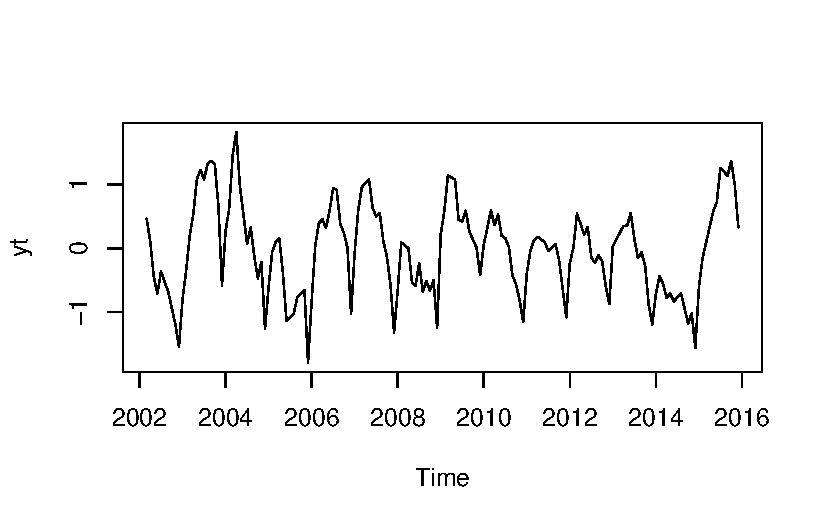
\includegraphics{ferramentas_files/figure-pdf/unnamed-chunk-7-1.pdf}

}

\end{figure}

\begin{Shaded}
\begin{Highlighting}[]
\FunctionTok{acf}\NormalTok{(yt, }\AttributeTok{lag =} \DecValTok{50}\NormalTok{)}
\end{Highlighting}
\end{Shaded}

\begin{figure}[H]

{\centering 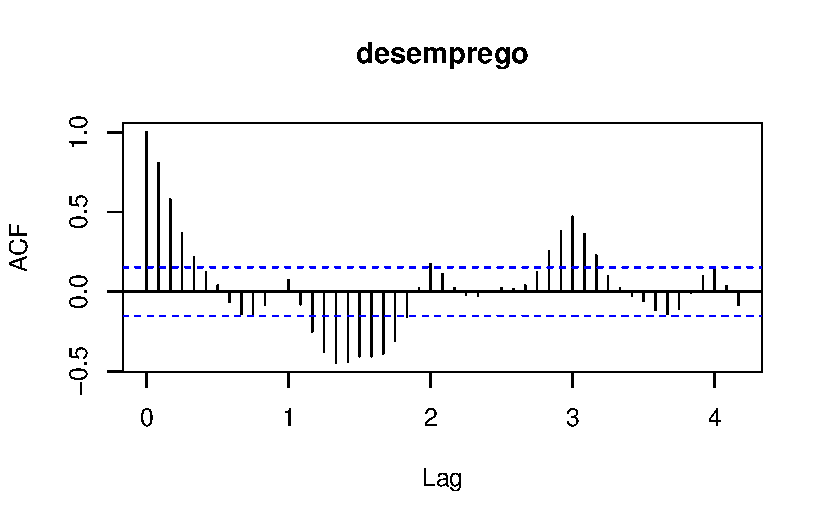
\includegraphics{ferramentas_files/figure-pdf/unnamed-chunk-7-2.pdf}

}

\end{figure}

Fica claro o comportamento sazonal. Note que o período não parece ser
anual, mas sim de 3 em 3 anos. Vamos avaliar esse aspecto com mais
detalhes na próxima seção.

\hypertarget{exercuxedcios-1}{%
\subsection{Exercícios}\label{exercuxedcios-1}}

Exercício 1 Considerando o banco de dados sobre suicídios no Mato Grosso
do Sul:

\begin{enumerate}
\def\labelenumi{\arabic{enumi}.}
\item
  Estime a tendência
\item
  Remova a tendência estimada e verifique se o resultado é um ruído
  branco
\end{enumerate}

Exercício 2 Verifique se há tendência na série \texttt{ldeaths}.

Exercício 3 Verifique se há tendência na série de óbitos maternos, cuja
url é

\begin{Shaded}
\begin{Highlighting}[]
\NormalTok{url }\OtherTok{\textless{}{-}} \StringTok{\textquotesingle{}https://drive.google.com/uc?authuser=0\&id=1tYFFT9L2iopKmBDUI3P8qNIRaOnMYj7d\&export=download\textquotesingle{}}
\end{Highlighting}
\end{Shaded}

Faça duas análises, uma com a série inteira e outra eliminando os dados
a partir de 2020.

Exercício 4. O banco de dados abaixo apresenta algumas séries temporais
mensais com o número de nascidos vivos em Manaus

\begin{Shaded}
\begin{Highlighting}[]
\NormalTok{url }\OtherTok{\textless{}{-}} \StringTok{\textquotesingle{}https://drive.google.com/uc?authuser=0\&id=139h6x2g7PkAHNTzsbQKUl5G2MqoXYk6Y\&export=download\textquotesingle{}}
\end{Highlighting}
\end{Shaded}

\begin{enumerate}
\def\labelenumi{\arabic{enumi}.}
\item
  Estime a tendência dos nascimentos considerando duas séries: partos
  vaginais e cesários. Coloque as duas informações no mesmo gráfico.
\item
  Elimine a tendência de cada série e verifique se há outro sinal a ser
  estimado.
\end{enumerate}

Exercício 1

\hypertarget{o-periodograma}{%
\section{O periodograma}\label{o-periodograma}}

\hypertarget{introduuxe7uxe3o-1}{%
\subsection{Introdução}\label{introduuxe7uxe3o-1}}

Todo padrão sazonal possui um período - a quantidade de tempo necessária
para que o padrão se repita. O inverso desse período é denominado
frequência fundamental, que é a fração de um ciclo por unidade de tempo.

\textbf{Exemplo:} Considere o período de 12 meses. Então, a frequência
fundamental é 1/12 (ou seja, cada mês representa um doze ávos do período
de 1 ano).

Lembremos que o sinal harmônico é igual a
\[\hbox{sinal}(t)=A\sin\left(2\pi\omega t+\phi\right),\] onde
\(\omega=1/p\) é a frequência. Com um pouco de trigonometria, podemos
mostrar que

\[\hbox{sinal}(t)=\beta_1\cos\left(2\pi\omega t\right)+ \beta_2\sin\left(2\pi\omega t\right)\]
onde \(\beta_1=A\cos(\phi)\) e \(\beta_2=-A\sin(\phi)\). É possível
mostrar também que \(A=\sqrt{\beta_1+\beta_2}\) e
\(\phi=\cos^{-1}(\beta_1/A)\). A vantagem dessa nova forma é que o sinal
pode ser escrito como um modelo linear e pode ser estimado facilmente. A
soma de quadrados explicada pela regressão é proporcional à

\[I(\omega)=\hat{A}(\omega)^2 \] e podemos mostrar que a estimativa de
máxima verossimilhança para \(\omega\) é o valor que maximiza
\(I(\omega)\).

Periodograma O gráfico de \(I(\omega)\) é denominado periodograma.

Vamos criar a função periodograma

\begin{Shaded}
\begin{Highlighting}[]
\NormalTok{Iw }\OtherTok{\textless{}{-}} \ControlFlowTok{function}\NormalTok{(y,w)\{}

  \CommentTok{\# matriz de planetamento}
\NormalTok{  n }\OtherTok{\textless{}{-}} \FunctionTok{length}\NormalTok{(y)}
\NormalTok{  t }\OtherTok{\textless{}{-}} \DecValTok{1}\SpecialCharTok{:}\NormalTok{n}
\NormalTok{  x }\OtherTok{\textless{}{-}} \FunctionTok{cbind}\NormalTok{(}\FunctionTok{cos}\NormalTok{(}\DecValTok{2}\SpecialCharTok{*}\NormalTok{pi}\SpecialCharTok{*}\NormalTok{w}\SpecialCharTok{*}\NormalTok{t), }\FunctionTok{sin}\NormalTok{(}\DecValTok{2}\SpecialCharTok{*}\NormalTok{pi}\SpecialCharTok{*}\NormalTok{w}\SpecialCharTok{*}\NormalTok{t))}
  
  \CommentTok{\# coeficientes do modelo linear}
\NormalTok{  beta }\OtherTok{\textless{}{-}} \FunctionTok{coefficients}\NormalTok{(}\FunctionTok{lm}\NormalTok{(y }\SpecialCharTok{\textasciitilde{}}\NormalTok{x}\DecValTok{{-}1}\NormalTok{))}
  
  \CommentTok{\# amplitude}
\NormalTok{  A }\OtherTok{\textless{}{-}} \FunctionTok{sqrt}\NormalTok{(}\FunctionTok{sum}\NormalTok{(beta}\SpecialCharTok{\^{}}\DecValTok{2}\NormalTok{))}
  
  \CommentTok{\# Iw}
\NormalTok{  .}\DecValTok{5}\SpecialCharTok{*}\NormalTok{n}\SpecialCharTok{*}\NormalTok{A}\SpecialCharTok{\^{}}\DecValTok{2}
\NormalTok{\}}

\NormalTok{periodograma }\OtherTok{\textless{}{-}} \ControlFlowTok{function}\NormalTok{(y)\{}
  \CommentTok{\# gráfico}
\NormalTok{  n }\OtherTok{\textless{}{-}} \FunctionTok{length}\NormalTok{(y)}
\NormalTok{  w\_detec }\OtherTok{\textless{}{-}}\NormalTok{ ( }\DecValTok{1} \SpecialCharTok{:} \FunctionTok{floor}\NormalTok{(  (n}\DecValTok{{-}1}\NormalTok{)}\SpecialCharTok{/} \DecValTok{2}\NormalTok{) ) }\SpecialCharTok{/}\NormalTok{ n}
\NormalTok{  I\_w }\OtherTok{\textless{}{-}} \FunctionTok{sapply}\NormalTok{( w\_detec, }\ControlFlowTok{function}\NormalTok{(w) }\FunctionTok{Iw}\NormalTok{(y , w) )}
  \FunctionTok{plot}\NormalTok{( }\DecValTok{1} \SpecialCharTok{/}\NormalTok{ w\_detec , I\_w, }\AttributeTok{xlab =} \StringTok{\textquotesingle{}Período\textquotesingle{}}\NormalTok{, }\AttributeTok{ylab =}     \FunctionTok{expression}\NormalTok{(}\FunctionTok{I}\NormalTok{(w)), }\AttributeTok{type =} \StringTok{\textquotesingle{}h\textquotesingle{}}\NormalTok{ , }\AttributeTok{lwd =} \DecValTok{2}\NormalTok{)}
  
  \CommentTok{\# encontrando o periodo}
\NormalTok{  fund }\OtherTok{\textless{}{-}}\NormalTok{  w\_detec[ }\FunctionTok{which}\NormalTok{( I\_w }\SpecialCharTok{==} \FunctionTok{max}\NormalTok{(I\_w))]}
  \FunctionTok{cat}\NormalTok{(}\StringTok{\textquotesingle{}Período: \textquotesingle{}}\NormalTok{,}\DecValTok{1}\SpecialCharTok{/}\NormalTok{fund,}\StringTok{\textquotesingle{}}\SpecialCharTok{\textbackslash{}n}\StringTok{\textquotesingle{}}\NormalTok{)}

\NormalTok{\}}
\end{Highlighting}
\end{Shaded}

Na função acima \texttt{y} é a série temporal. Vamos aplicar essa função
para a série de temperaturas no Castelo de Nottingham.

\begin{Shaded}
\begin{Highlighting}[]
\FunctionTok{periodograma}\NormalTok{(nottem)}
\end{Highlighting}
\end{Shaded}

\begin{figure}[H]

{\centering 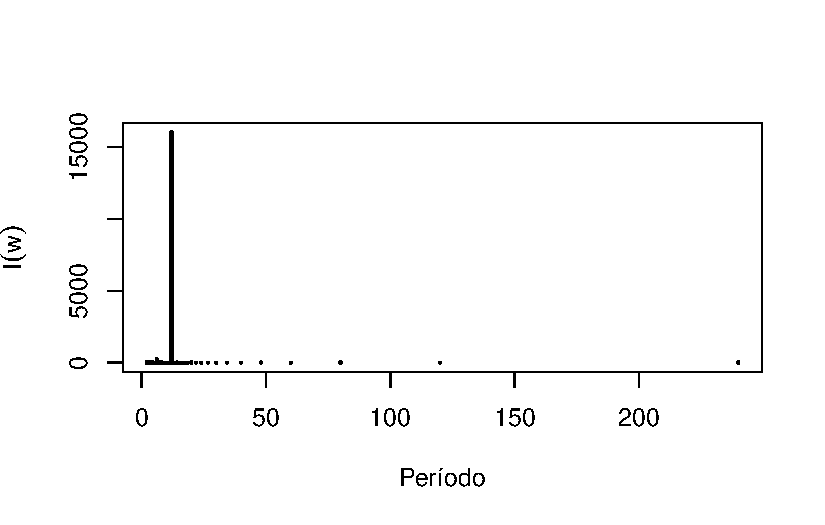
\includegraphics{ferramentas_files/figure-pdf/unnamed-chunk-11-1.pdf}

}

\end{figure}

\begin{verbatim}
Período:  12 
\end{verbatim}

\hypertarget{periodograma-para-amostras-aleatuxf3rias}{%
\subsection{Periodograma para amostras
aleatórias}\label{periodograma-para-amostras-aleatuxf3rias}}

É importante notar que a frequência fundamental é um pico expressivo em
relação aos demais. Abaixo mostramos o periodograma para uma amostra
aleatória - note como há vários picos, evidenciando a falta de uma
frequência fundamental.

\begin{Shaded}
\begin{Highlighting}[]
\FunctionTok{periodograma}\NormalTok{(}\FunctionTok{rnorm}\NormalTok{(}\DecValTok{100}\NormalTok{))}
\end{Highlighting}
\end{Shaded}

\begin{figure}[H]

{\centering 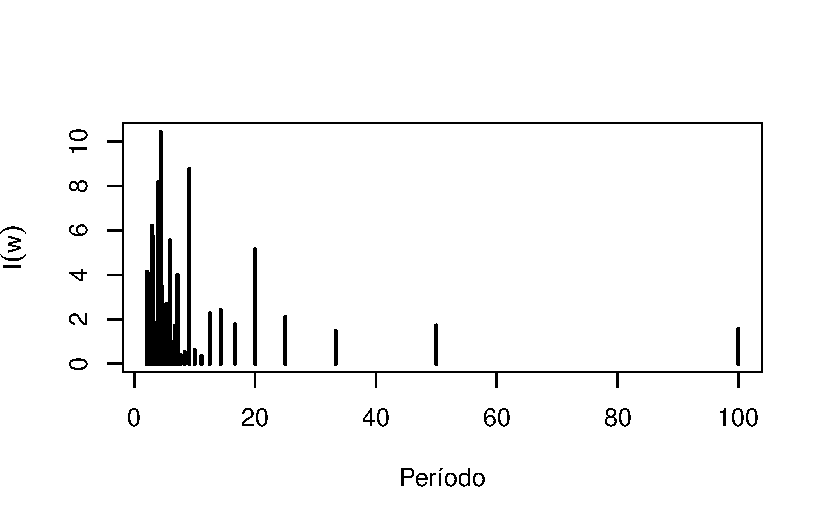
\includegraphics{ferramentas_files/figure-pdf/unnamed-chunk-12-1.pdf}

}

\end{figure}

\begin{verbatim}
Período:  2.631579 
\end{verbatim}

\hypertarget{periodograma-na-presenuxe7a-de-tenduxeancia}{%
\subsection{Periodograma na presença de
tendência}\label{periodograma-na-presenuxe7a-de-tenduxeancia}}

É importante remover a tendência antes de aplicar o periodo. Por
exemplo, considere novamente a série \texttt{AirPassengers}

\begin{Shaded}
\begin{Highlighting}[]
\FunctionTok{ts.plot}\NormalTok{(AirPassengers)}
\end{Highlighting}
\end{Shaded}

\begin{figure}[H]

{\centering \includegraphics{ferramentas_files/figure-pdf/unnamed-chunk-13-1.pdf}

}

\end{figure}

\begin{Shaded}
\begin{Highlighting}[]
\FunctionTok{periodograma}\NormalTok{(AirPassengers)}
\end{Highlighting}
\end{Shaded}

\begin{figure}[H]

{\centering \includegraphics{ferramentas_files/figure-pdf/unnamed-chunk-13-2.pdf}

}

\end{figure}

\begin{verbatim}
Período:  144 
\end{verbatim}

Embor exista uma sazonalidade clara, o periodograma retorna um período
de 12 anos, algo irreal. Vamos remover a tendência.

\begin{Shaded}
\begin{Highlighting}[]
\CommentTok{\# criando o loess}
\NormalTok{y }\OtherTok{\textless{}{-}}\NormalTok{ AirPassengers}
\NormalTok{tempo }\OtherTok{\textless{}{-}} \DecValTok{1}\SpecialCharTok{:}\FunctionTok{length}\NormalTok{(y)}
\NormalTok{lw }\OtherTok{\textless{}{-}} \FunctionTok{loess}\NormalTok{( y }\SpecialCharTok{\textasciitilde{}}\NormalTok{ tempo )}
\NormalTok{fit }\OtherTok{\textless{}{-}}\NormalTok{ lw}\SpecialCharTok{$}\NormalTok{fitted}

\CommentTok{\# criando a série livre de tendência}
\NormalTok{y\_detrend }\OtherTok{\textless{}{-}} \FunctionTok{ts}\NormalTok{( y}\SpecialCharTok{{-}}\NormalTok{fit, }\AttributeTok{start =} \FunctionTok{start}\NormalTok{(y), }\AttributeTok{frequency =} \FunctionTok{frequency}\NormalTok{(y))}

\FunctionTok{ts.plot}\NormalTok{( y\_detrend )}
\end{Highlighting}
\end{Shaded}

\begin{figure}[H]

{\centering 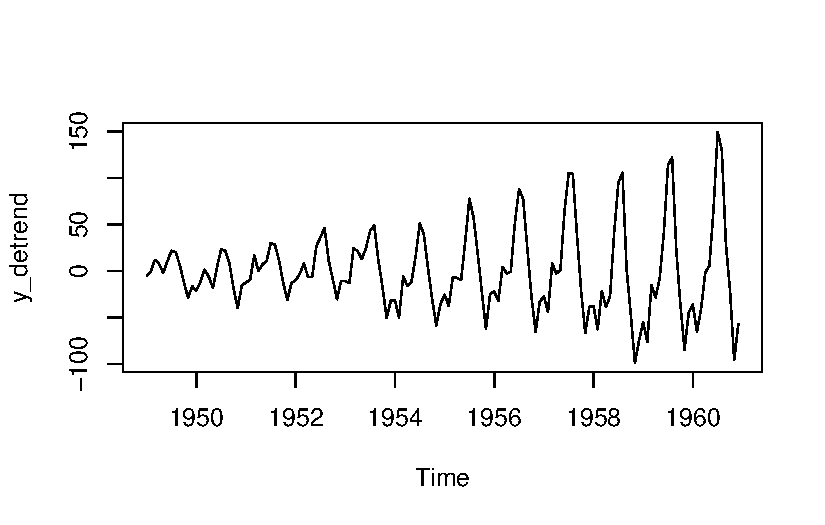
\includegraphics{ferramentas_files/figure-pdf/unnamed-chunk-14-1.pdf}

}

\end{figure}

\begin{Shaded}
\begin{Highlighting}[]
\FunctionTok{periodograma}\NormalTok{( y\_detrend )}
\end{Highlighting}
\end{Shaded}

\begin{figure}[H]

{\centering 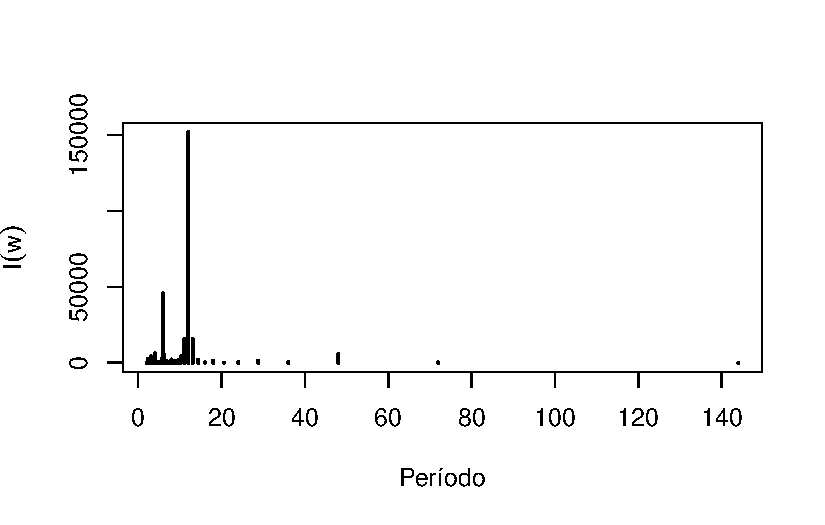
\includegraphics{ferramentas_files/figure-pdf/unnamed-chunk-14-2.pdf}

}

\end{figure}

\begin{verbatim}
Período:  12 
\end{verbatim}

\hypertarget{exercuxedcios-2}{%
\subsection{Exercícios}\label{exercuxedcios-2}}

Exercício 1. Determine o período da série \texttt{ldeaths} - número de
óbito mensais por doenças pulmonares no Reino Unido.

Exercício 2. Determine o período da série de óbitos maternos, cuja url
é:

\begin{Shaded}
\begin{Highlighting}[]
\NormalTok{url }\OtherTok{\textless{}{-}} \StringTok{\textquotesingle{}https://drive.google.com/uc?authuser=0\&id=1tYFFT9L2iopKmBDUI3P8qNIRaOnMYj7d\&export=download\textquotesingle{}}
\end{Highlighting}
\end{Shaded}

Exercício 3. A série \texttt{co2} representa a concentração de CO\(_2\)
na atmosfera medida em Mauna Loa. Analise a tendência da série e estime
o período.

Exercício 4. Determine a tendência e o período da série mensal do número
de nascidos vivos em Manaus, independente do tipo de parto.

\hypertarget{ajuste-por-fatores-sazonais}{%
\section{Ajuste por fatores
sazonais}\label{ajuste-por-fatores-sazonais}}

Considere novamente o harmônico

\[\hbox{sinal}(t)=A\cos\left(\frac{2\pi}{p}t+\phi\right)\]

O sinal no tempo \(t=1+p\) é equivalente ao sinal no tempo 1:

\[\hbox{sinal}(1+p)=A\cos\left(\frac{2\pi}{p}+2\pi+\phi\right)=A\cos\left(\frac{2\pi}{p}+\phi\right)=\hbox{sinal}(1)\]

Isso é verdade para todo \(t=1+kp\), onde \(k=1,2,\ldots.\) Isto implica
que, na prática, a imagem de \(\hbox{sinal}(t)\) só pode ser \(p\)
valores:

\[\hbox{sinal}(t)=\left\{\begin{array}{ll}\hbox{sinal}(1),&t=1,1+p,1+2p,\ldots,\\
\hbox{sinal}(2),&t=2,2+p,2+2p\ldots,\\
\vdots,&\vdots\\
\hbox{sinal}(p),&t=p,2p,3p\ldots,\end{array}\right.\]

Então \[x_t=\hbox{sinal}(t)+\varepsilon_t\] pode ser considerado uma
ANOVA com um fator.

Considere a série \texttt{ldeths}, que já sabemos ter uma leve tendência
decrescente e sazonalidade com período 12. Primeiro, vamos encontrar a
série livre de tendência:

\begin{Shaded}
\begin{Highlighting}[]
\NormalTok{tempo }\OtherTok{\textless{}{-}} \DecValTok{1}\SpecialCharTok{:}\FunctionTok{length}\NormalTok{(ldeaths)}
\NormalTok{lw }\OtherTok{\textless{}{-}} \FunctionTok{loess}\NormalTok{( ldeaths }\SpecialCharTok{\textasciitilde{}}\NormalTok{ tempo)}
\NormalTok{tend }\OtherTok{\textless{}{-}}\NormalTok{ lw}\SpecialCharTok{$}\NormalTok{fitted}

\NormalTok{tend }\OtherTok{\textless{}{-}} \FunctionTok{ts}\NormalTok{( tend, }\AttributeTok{start =} \FunctionTok{start}\NormalTok{(ldeaths), }\AttributeTok{frequency =} \FunctionTok{frequency}\NormalTok{(ldeaths))}

\CommentTok{\#  série sem tendência}
\NormalTok{d\_ldeaths }\OtherTok{\textless{}{-}}\NormalTok{ ldeaths }\SpecialCharTok{{-}}\NormalTok{ tend}
\end{Highlighting}
\end{Shaded}

Em seguida, encontramos o período.

\begin{Shaded}
\begin{Highlighting}[]
\FunctionTok{periodograma}\NormalTok{(d\_ldeaths)}
\end{Highlighting}
\end{Shaded}

\begin{figure}[H]

{\centering 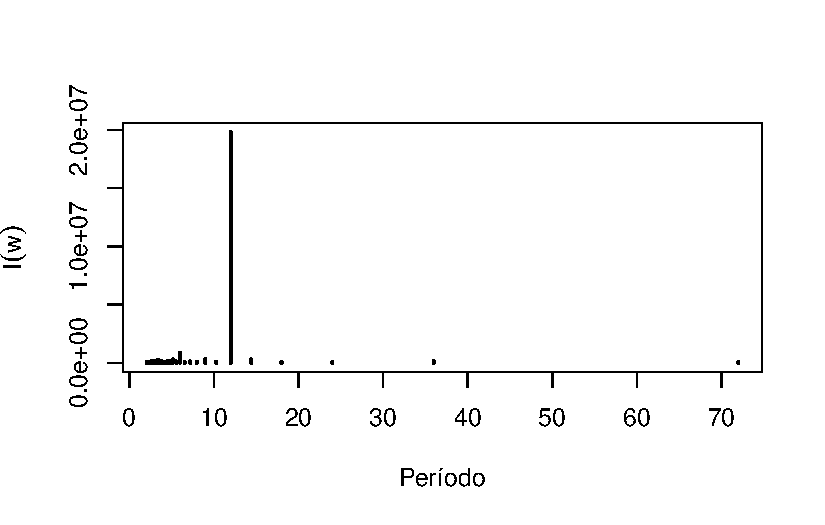
\includegraphics{ferramentas_files/figure-pdf/unnamed-chunk-17-1.pdf}

}

\end{figure}

\begin{verbatim}
Período:  12 
\end{verbatim}

Nesse momento, devemos atribuir o período para o objeto \texttt{ts},
fazendo

\begin{Shaded}
\begin{Highlighting}[]
\NormalTok{d\_ldeaths }\OtherTok{\textless{}{-}} \FunctionTok{ts}\NormalTok{( d\_ldeaths, }\AttributeTok{frequency=} \DecValTok{12}\NormalTok{) }
\end{Highlighting}
\end{Shaded}

Note que o código acima foi inócuo porque o objeto \texttt{ldeaths} já
tinha o período 12.

Antes de fazer o ajuste sazonal, é possível fazer um gráfico com doze
séries temporais, uma para cada fator sazonal (no nosso exemplo, uma
série só de janeiros, de fevereiros, etc). Mostramos isso a seguir:

\begin{Shaded}
\begin{Highlighting}[]
\FunctionTok{monthplot}\NormalTok{(d\_ldeaths)}
\end{Highlighting}
\end{Shaded}

\begin{figure}[H]

{\centering 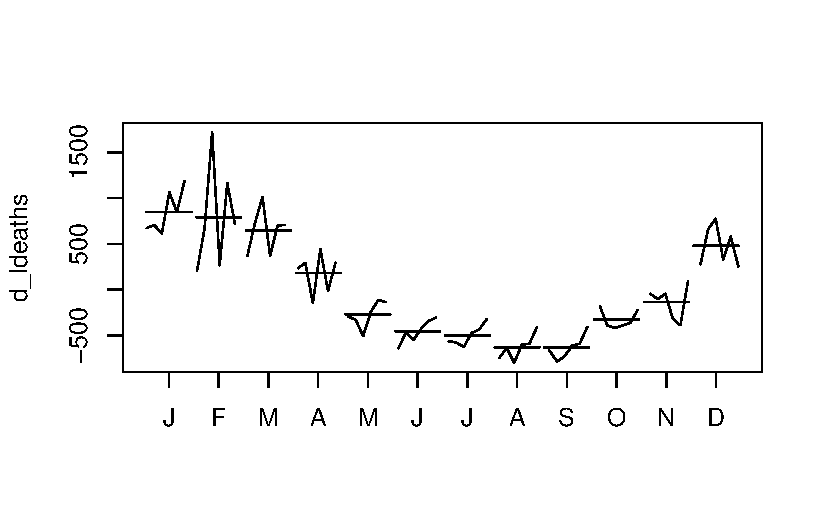
\includegraphics{ferramentas_files/figure-pdf/unnamed-chunk-19-1.pdf}

}

\end{figure}

No gráfico acima, a linha horizontal em cada mês representa a média.

Agora, vamos estimar os 12 fatores sazonais. Para isso, vamos utilizar a
função \texttt{cycle}, que mostra a posição de cada observação dentro do
ciclo sazonal. Eis um exemplo de seu funcionamento:

\begin{Shaded}
\begin{Highlighting}[]
\FunctionTok{head}\NormalTok{(}\FunctionTok{cycle}\NormalTok{(d\_ldeaths), }\DecValTok{14}\NormalTok{)}
\end{Highlighting}
\end{Shaded}

\begin{verbatim}
 [1]  1  2  3  4  5  6  7  8  9 10 11 12  1  2
\end{verbatim}

Vamos transformar o resultado do \texttt{cycle} em um fator e ajustar
uma ANOVA:

\begin{Shaded}
\begin{Highlighting}[]
\NormalTok{ciclo }\OtherTok{\textless{}{-}} \FunctionTok{as.factor}\NormalTok{(}\FunctionTok{cycle}\NormalTok{(d\_ldeaths))}
\NormalTok{mod }\OtherTok{\textless{}{-}} \FunctionTok{lm}\NormalTok{( d\_ldeaths }\SpecialCharTok{\textasciitilde{}}\NormalTok{ciclo}\DecValTok{{-}1}\NormalTok{)}

\FunctionTok{plot}\NormalTok{(}\FunctionTok{coefficients}\NormalTok{(mod))}
\end{Highlighting}
\end{Shaded}

\begin{figure}[H]

{\centering 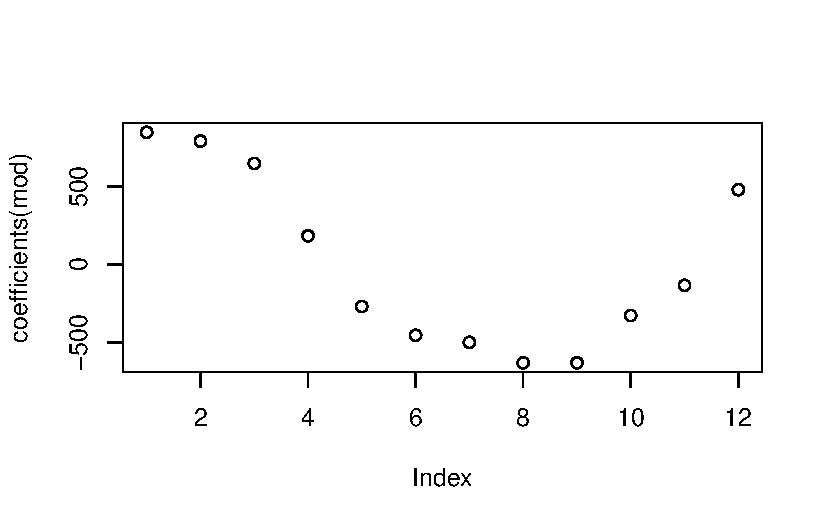
\includegraphics{ferramentas_files/figure-pdf/unnamed-chunk-21-1.pdf}

}

\end{figure}

Por último, vamos dessazonalizar a série:

\begin{Shaded}
\begin{Highlighting}[]
\NormalTok{saz\_fit }\OtherTok{\textless{}{-}}\NormalTok{ mod}\SpecialCharTok{$}\NormalTok{fitted.values}
\NormalTok{residuo }\OtherTok{\textless{}{-}}\NormalTok{ d\_ldeaths }\SpecialCharTok{{-}}\NormalTok{ saz\_fit}

\FunctionTok{plot}\NormalTok{(residuo)}
\end{Highlighting}
\end{Shaded}

\begin{figure}[H]

{\centering 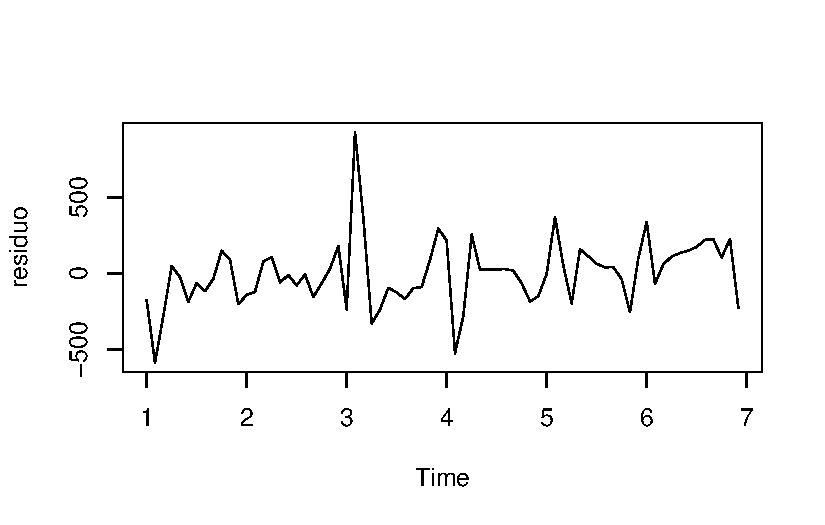
\includegraphics{ferramentas_files/figure-pdf/unnamed-chunk-22-1.pdf}

}

\end{figure}

\begin{Shaded}
\begin{Highlighting}[]
\FunctionTok{acf}\NormalTok{(residuo, }\AttributeTok{lag =} \DecValTok{30}\NormalTok{)}
\end{Highlighting}
\end{Shaded}

\begin{figure}[H]

{\centering 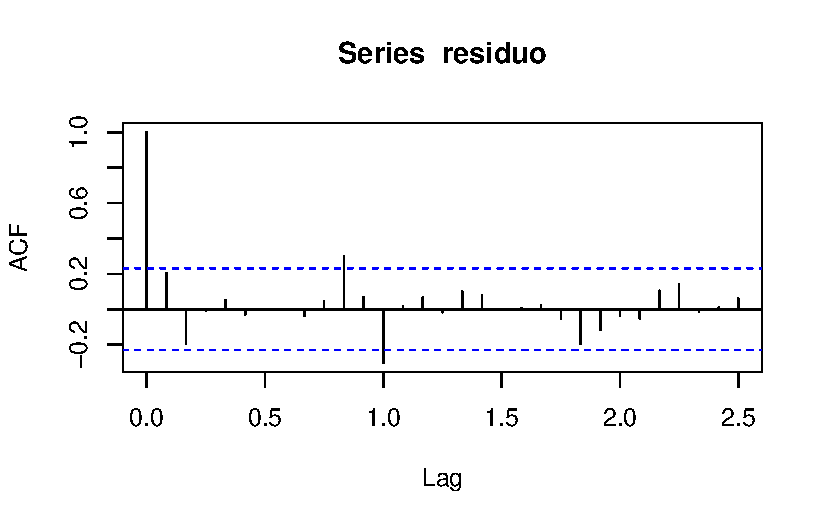
\includegraphics{ferramentas_files/figure-pdf/unnamed-chunk-22-2.pdf}

}

\end{figure}

\hypertarget{exercuxedcios-3}{%
\subsection{Exercícios}\label{exercuxedcios-3}}

\bookmarksetup{startatroot}

\hypertarget{o-modelo-linear-dinuxe2mico}{%
\chapter{O modelo linear dinâmico}\label{o-modelo-linear-dinuxe2mico}}

\hypertarget{o-modelo-linear-dinuxe2mico-1}{%
\section{O modelo linear dinâmico}\label{o-modelo-linear-dinuxe2mico-1}}

Seja \(y_1,\ldots,t\) uma série temporal. Seja \(D_j={y_1,\ldots,y_j}\).
Dizemos que \(y_t\) é um modelo linear dinâmico se

\[\begin{align}
y_t|\boldsymbol{\theta}_t,D_{t-1}&\sim\hbox{Normal}(\boldsymbol{F}_t'\boldsymbol{\theta}_t,V_t)\\
\boldsymbol{\theta}_t|\boldsymbol{\theta}_{t-1},D_{t-1}&\sim\hbox{Normal}(\boldsymbol{G}_t\boldsymbol{\theta}_{t-1},\boldsymbol{W}_t)
\end{align}\]

A expressão acima, os \(\theta\)'s são denominados estados. Para a
completa especificação do modelo, devemos informar valores iniciais
\(m_0\) e \(C_0\) que representam nossa opinião sobre os estados antes
do tempo \(1\):

\[\theta_0\sim\ N(m_0,C_0)\] Escolhas diferentes para
\(\boldsymbol{F}_t\) e \(\boldsymbol{G}_t\) permitem acomodar sinais
diferentes.

Pode-se mostrar que \(y_{t+h}|D_t\) tem distribuição normal. Como
\(t+h\) é um tempo não observado, essa é a distribuição para previsões.
Neste caso, a função de previsão para o horizonte \(h\) é

\[f_t(h)=E(Y_{t+h}|D_{t})\] onde \(E(.)\) sempre deve ser lido como
\textbf{média}.

O pacote para lidar com modelos lineares dinâmicos é o \texttt{dlm}. A
função abaixo é utilizada para estimar as variâncias desconhecidas do
modelo e deve sempre ser colocada no \emph{environment} do \texttt{R}:

\begin{Shaded}
\begin{Highlighting}[]
\FunctionTok{require}\NormalTok{(dlm)}
\end{Highlighting}
\end{Shaded}

\begin{verbatim}
Carregando pacotes exigidos: dlm
\end{verbatim}

\begin{verbatim}
Warning: package 'dlm' was built under R version 4.3.1
\end{verbatim}

\begin{Shaded}
\begin{Highlighting}[]
\NormalTok{modFim }\OtherTok{\textless{}{-}} \ControlFlowTok{function}\NormalTok{(y,mod)\{}
\NormalTok{  ffbs }\OtherTok{\textless{}{-}} \FunctionTok{dlmGibbsDIG}\NormalTok{(y, }\AttributeTok{mod =}\NormalTok{ mod, }\AttributeTok{n.sample =} \DecValTok{5000}\NormalTok{,}
                    \AttributeTok{a.y=}\DecValTok{1}\NormalTok{,}\AttributeTok{b.y=}\DecValTok{100}\NormalTok{,}\AttributeTok{a.theta=}\DecValTok{1}\NormalTok{,}\AttributeTok{b.theta=}\DecValTok{100}\NormalTok{,}
                    \AttributeTok{save.states =} \ConstantTok{FALSE}\NormalTok{, }\AttributeTok{thin =} \DecValTok{0}\NormalTok{)}

\NormalTok{v\_sim  }\OtherTok{\textless{}{-}} \FunctionTok{sample}\NormalTok{(ffbs}\SpecialCharTok{$}\NormalTok{dV[}\SpecialCharTok{{-}}\NormalTok{(}\DecValTok{1}\SpecialCharTok{:}\DecValTok{2500}\NormalTok{)],}\DecValTok{2500}\NormalTok{,T)}

\NormalTok{q }\OtherTok{\textless{}{-}} \FunctionTok{dim}\NormalTok{(ffbs}\SpecialCharTok{$}\NormalTok{dW)[}\DecValTok{2}\NormalTok{]}
\NormalTok{w\_sim }\OtherTok{\textless{}{-}} \ConstantTok{NULL}
\ControlFlowTok{for}\NormalTok{(j }\ControlFlowTok{in} \DecValTok{1}\SpecialCharTok{:}\NormalTok{q)\{}
\NormalTok{ w\_sim }\OtherTok{\textless{}{-}} \FunctionTok{c}\NormalTok{(w\_sim, }\FunctionTok{mean}\NormalTok{(}\FunctionTok{sample}\NormalTok{(ffbs}\SpecialCharTok{$}\NormalTok{dW[,j][}\SpecialCharTok{{-}}\NormalTok{(}\DecValTok{1}\SpecialCharTok{:}\DecValTok{2500}\NormalTok{)],}\DecValTok{2500}\NormalTok{,T)))}
\NormalTok{\}}
\CommentTok{\# declarando as variâncias na quádrupla}
\NormalTok{mod}\SpecialCharTok{$}\NormalTok{V }\OtherTok{\textless{}{-}} \FunctionTok{mean}\NormalTok{(v\_sim)}
\NormalTok{mod}\SpecialCharTok{$}\NormalTok{W }\OtherTok{\textless{}{-}} \FunctionTok{diag}\NormalTok{( w\_sim)}
\FunctionTok{return}\NormalTok{(mod)}
\NormalTok{\}}
\end{Highlighting}
\end{Shaded}

Também pode-se mostrar que \(\theta_{t-h}|D_t\) tem distribuição normal.
Como se trata da distribuição dos estados após verificar toda a série
temporal, esta é a distribuição para a suavização.

\bookmarksetup{startatroot}

\hypertarget{modelo-linear-dinuxe2mico-polinomial}{%
\chapter{Modelo linear dinâmico
polinomial}\label{modelo-linear-dinuxe2mico-polinomial}}

\begin{Shaded}
\begin{Highlighting}[]
\FunctionTok{require}\NormalTok{(dlm)}
\end{Highlighting}
\end{Shaded}

\begin{verbatim}
Carregando pacotes exigidos: dlm
\end{verbatim}

\begin{verbatim}
Warning: package 'dlm' was built under R version 4.3.1
\end{verbatim}

\begin{Shaded}
\begin{Highlighting}[]
\NormalTok{modFim }\OtherTok{\textless{}{-}} \ControlFlowTok{function}\NormalTok{(y,mod)\{}

\NormalTok{    ffbs }\OtherTok{\textless{}{-}} \FunctionTok{dlmGibbsDIG}\NormalTok{(y, }\AttributeTok{mod =}\NormalTok{ mod, }\AttributeTok{n.sample =} \DecValTok{5000}\NormalTok{,}
                    \AttributeTok{a.y=}\DecValTok{1}\NormalTok{,}\AttributeTok{b.y=}\DecValTok{100}\NormalTok{,}\AttributeTok{a.theta=}\DecValTok{1}\NormalTok{,}\AttributeTok{b.theta=}\DecValTok{100}\NormalTok{,}
                    \AttributeTok{save.states =} \ConstantTok{FALSE}\NormalTok{, }\AttributeTok{thin =} \DecValTok{0}\NormalTok{)}

\NormalTok{v\_sim  }\OtherTok{\textless{}{-}} \FunctionTok{sample}\NormalTok{(ffbs}\SpecialCharTok{$}\NormalTok{dV[}\SpecialCharTok{{-}}\NormalTok{(}\DecValTok{1}\SpecialCharTok{:}\DecValTok{2500}\NormalTok{)],}\DecValTok{2500}\NormalTok{,T)}

\NormalTok{q }\OtherTok{\textless{}{-}} \FunctionTok{dim}\NormalTok{(ffbs}\SpecialCharTok{$}\NormalTok{dW)[}\DecValTok{2}\NormalTok{]}
\NormalTok{w\_sim }\OtherTok{\textless{}{-}} \ConstantTok{NULL}
\ControlFlowTok{for}\NormalTok{(j }\ControlFlowTok{in} \DecValTok{1}\SpecialCharTok{:}\NormalTok{q)\{}
\NormalTok{ w\_sim }\OtherTok{\textless{}{-}} \FunctionTok{c}\NormalTok{(w\_sim, }\FunctionTok{mean}\NormalTok{(}\FunctionTok{sample}\NormalTok{(ffbs}\SpecialCharTok{$}\NormalTok{dW[,j][}\SpecialCharTok{{-}}\NormalTok{(}\DecValTok{1}\SpecialCharTok{:}\DecValTok{2500}\NormalTok{)],}\DecValTok{2500}\NormalTok{,T)))}
\NormalTok{\}}
\CommentTok{\# declarando as variâncias na quádrupla}
\NormalTok{mod}\SpecialCharTok{$}\NormalTok{V }\OtherTok{\textless{}{-}} \FunctionTok{mean}\NormalTok{(v\_sim)}
\NormalTok{mod}\SpecialCharTok{$}\NormalTok{W }\OtherTok{\textless{}{-}} \FunctionTok{diag}\NormalTok{( w\_sim,q)}
\FunctionTok{return}\NormalTok{(mod)}
\NormalTok{\}}
\end{Highlighting}
\end{Shaded}

Os modelos linearas dinâmicos polinomiais possuem uma função de previsão
polinomial.

Os podemos mais utilizados na prática são os de ordem 1 e 2, também
conhecidos como modelo de nível e de tendência linear, respectivamente.

\hypertarget{o-modelo-de-nuxedvel}{%
\section{O modelo de nível}\label{o-modelo-de-nuxedvel}}

O modelo de ordem 1, também conhecido como modelo de nível, possui
função de previsão da forma

\[f_t(h)=m_t,\] onde \(m_t\) é a média da série para o tempo \(t\). Esse
tipo de modelo é útil para séries temporais que possuem oscilações na
média (ou nível) mas sem exibir uma tendência forte.

Considere, por exemplo, a série com valores anuais das cheias do Rio
Nilo entre 1871 e 1970.

\begin{Shaded}
\begin{Highlighting}[]
\NormalTok{Nile }\OtherTok{\textless{}{-}} \FunctionTok{ts}\NormalTok{(Nile, }\AttributeTok{start =}\DecValTok{1900}\NormalTok{)}
\FunctionTok{ts.plot}\NormalTok{(Nile, }\AttributeTok{lwd =} \DecValTok{2}\NormalTok{)}
\end{Highlighting}
\end{Shaded}

\begin{figure}[H]

{\centering \includegraphics{polinomial_files/figure-pdf/unnamed-chunk-2-1.pdf}

}

\end{figure}

\begin{Shaded}
\begin{Highlighting}[]
\FunctionTok{acf}\NormalTok{(Nile, }\AttributeTok{lwd =} \DecValTok{2}\NormalTok{)}
\end{Highlighting}
\end{Shaded}

\begin{figure}[H]

{\centering 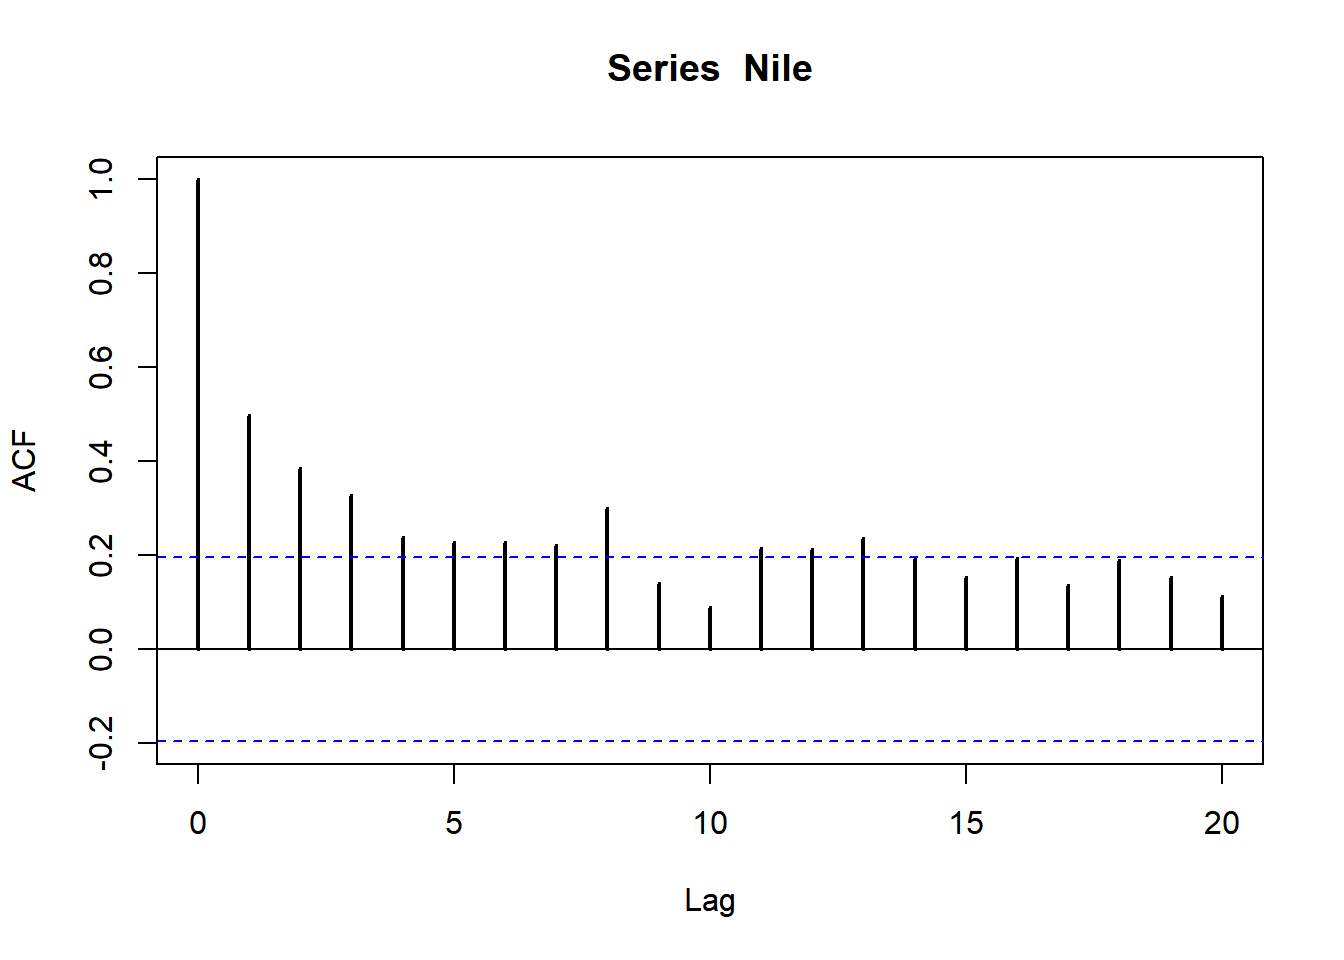
\includegraphics{polinomial_files/figure-pdf/unnamed-chunk-2-2.pdf}

}

\end{figure}

É possível notar que há autocorrelação na série, mas o correlograma não
revela uma tendência forte. Abaixo mostramos a tendência estimada via
\texttt{loess}.

\begin{Shaded}
\begin{Highlighting}[]
\NormalTok{tempo }\OtherTok{\textless{}{-}} \DecValTok{1}\SpecialCharTok{:}\FunctionTok{length}\NormalTok{(Nile)}
\NormalTok{lw }\OtherTok{\textless{}{-}} \FunctionTok{loess}\NormalTok{( Nile }\SpecialCharTok{\textasciitilde{}}\NormalTok{ tempo)}
\NormalTok{tend }\OtherTok{\textless{}{-}} \FunctionTok{ts}\NormalTok{(lw}\SpecialCharTok{$}\NormalTok{fitted, }\AttributeTok{start =} \FunctionTok{start}\NormalTok{(Nile))}

\FunctionTok{ts.plot}\NormalTok{(Nile)}
\FunctionTok{lines}\NormalTok{(tend, }\AttributeTok{lwd =} \DecValTok{2}\NormalTok{, }\AttributeTok{col =} \StringTok{\textquotesingle{}tomato\textquotesingle{}}\NormalTok{)}
\end{Highlighting}
\end{Shaded}

\begin{figure}[H]

{\centering \includegraphics{polinomial_files/figure-pdf/unnamed-chunk-3-1.pdf}

}

\end{figure}

A tendência estimada via \texttt{loess} parece revelar um comportamento
inicial de queda e depois meio século de valores oscilando em torno de
do nível. Vamos analisar isso utilizando um modelo linear dinâmico para
o nível.

Primeiro, vamos criar um objeto que possui os componentes \(F\) e \(G\)
adequados. Para tanto, basta usar a função \texttt{dlmPoly} e escolher a
ordem do modelo polinomial.

\begin{Shaded}
\begin{Highlighting}[]
\FunctionTok{library}\NormalTok{(dlm)}
\NormalTok{mod }\OtherTok{\textless{}{-}} \FunctionTok{dlmModPoly}\NormalTok{( }\AttributeTok{order =} \DecValTok{1}\NormalTok{)}
\end{Highlighting}
\end{Shaded}

Se você tiver curiosidade, \(F\) e \(G\) estão guardados em lista, com
os nomes \texttt{FF} e \texttt{GG}

Dentro do objeto \texttt{mod} há um componente denomina \texttt{m0}. Ele
é a estimativa do nível antes de 1. Vamos simplesmente dizer que este é
igual ao valor observado em 1900

\begin{Shaded}
\begin{Highlighting}[]
\NormalTok{mod}\SpecialCharTok{$}\NormalTok{m0 }\OtherTok{\textless{}{-}}\NormalTok{ Nile[}\DecValTok{1}\NormalTok{]}
\end{Highlighting}
\end{Shaded}

Agora, vamos estimar as variâncias do modelo, para obter \(V\) e \(W\):

\begin{Shaded}
\begin{Highlighting}[]
\NormalTok{mod }\OtherTok{\textless{}{-}} \FunctionTok{modFim}\NormalTok{( Nile, mod)}
\end{Highlighting}
\end{Shaded}

Agora, vamos aplicar o Teorema de Bayes, através de uma série de
atualizações conhecidas como Filtro de Kalman

\begin{Shaded}
\begin{Highlighting}[]
\NormalTok{filtro }\OtherTok{\textless{}{-}} \FunctionTok{dlmFilter}\NormalTok{(Nile, mod)}
\end{Highlighting}
\end{Shaded}

Em modelos lineares dinâmicos, definimos o erro de previsão por

\[y_t-E(y_t|D_{t-1})=y_t-f_t.\] Se todos os sinais foram bem ajustados,
os erros de previsão possuem comportamento com um ruído branco. O valor
de \(f_t\) está no objeto \texttt{filtro}.

\begin{Shaded}
\begin{Highlighting}[]
\NormalTok{erro }\OtherTok{\textless{}{-}}\NormalTok{ Nile }\SpecialCharTok{{-}}\NormalTok{ filtro}\SpecialCharTok{$}\NormalTok{f}
\FunctionTok{ts.plot}\NormalTok{(erro)}
\end{Highlighting}
\end{Shaded}

\begin{figure}[H]

{\centering \includegraphics{polinomial_files/figure-pdf/unnamed-chunk-8-1.pdf}

}

\end{figure}

\begin{Shaded}
\begin{Highlighting}[]
\FunctionTok{acf}\NormalTok{(erro)}
\end{Highlighting}
\end{Shaded}

\begin{figure}[H]

{\centering 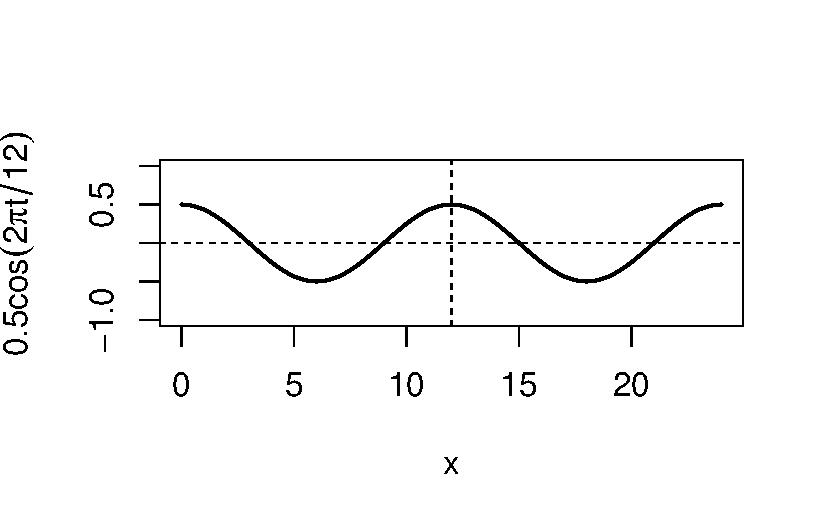
\includegraphics{polinomial_files/figure-pdf/unnamed-chunk-8-2.pdf}

}

\end{figure}

Agora, vamos reaplicar o Teorema de Bayes, considerando a amostra toda,
para obter a estimativa suavizada do nível.

\begin{Shaded}
\begin{Highlighting}[]
\NormalTok{suave }\OtherTok{\textless{}{-}} \FunctionTok{dlmSmooth}\NormalTok{(filtro)}

\FunctionTok{ts.plot}\NormalTok{(Nile)}
\FunctionTok{lines}\NormalTok{( suave}\SpecialCharTok{$}\NormalTok{s, }\AttributeTok{lwd =} \DecValTok{2}\NormalTok{, }\AttributeTok{col =} \StringTok{\textquotesingle{}seagreen\textquotesingle{}}\NormalTok{)}
\end{Highlighting}
\end{Shaded}

\begin{figure}[H]

{\centering 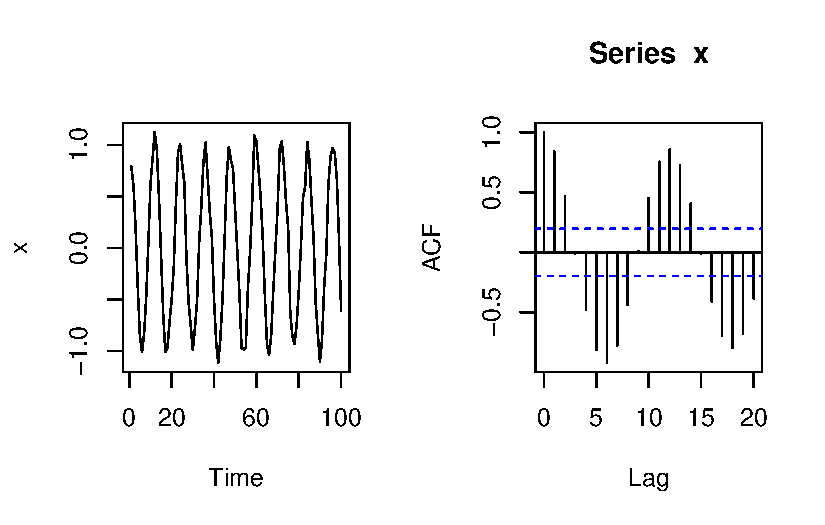
\includegraphics{polinomial_files/figure-pdf/unnamed-chunk-9-1.pdf}

}

\end{figure}

Também podemos fazer um intervalo de credibidade para o nível suavizado.

\begin{Shaded}
\begin{Highlighting}[]
\FunctionTok{ts.plot}\NormalTok{(Nile)}
\FunctionTok{lines}\NormalTok{( suave}\SpecialCharTok{$}\NormalTok{s, }\AttributeTok{lwd =} \DecValTok{2}\NormalTok{, }\AttributeTok{col =} \StringTok{\textquotesingle{}seagreen\textquotesingle{}}\NormalTok{)}

\CommentTok{\# variâncias da suavização}
\NormalTok{vs }\OtherTok{\textless{}{-}} \FunctionTok{dlmSvd2var}\NormalTok{(suave}\SpecialCharTok{$}\NormalTok{U.S, suave}\SpecialCharTok{$}\NormalTok{D.S)}

\CommentTok{\# intervalo de credibilidade}
\FunctionTok{lines}\NormalTok{( suave}\SpecialCharTok{$}\NormalTok{s }\SpecialCharTok{{-}} \FloatTok{1.96}\SpecialCharTok{*}\FunctionTok{sqrt}\NormalTok{(}\FunctionTok{unlist}\NormalTok{(vs)) )}
\FunctionTok{lines}\NormalTok{( suave}\SpecialCharTok{$}\NormalTok{s }\SpecialCharTok{+} \FloatTok{1.96}\SpecialCharTok{*}\FunctionTok{sqrt}\NormalTok{(}\FunctionTok{unlist}\NormalTok{(vs)) )}
\end{Highlighting}
\end{Shaded}

\begin{figure}[H]

{\centering \includegraphics{polinomial_files/figure-pdf/unnamed-chunk-10-1.pdf}

}

\end{figure}

Podemos fazer previsões com a função

\begin{Shaded}
\begin{Highlighting}[]
\NormalTok{prev }\OtherTok{\textless{}{-}} \FunctionTok{dlmForecast}\NormalTok{(filtro, }\DecValTok{3}\NormalTok{)}
\NormalTok{prev}\SpecialCharTok{$}\NormalTok{f}
\end{Highlighting}
\end{Shaded}

\begin{verbatim}
Time Series:
Start = 2000 
End = 2002 
Frequency = 1 
     Series 1
[1,]  792.767
[2,]  792.767
[3,]  792.767
\end{verbatim}

\hypertarget{o-modelo-de-tenduxeancia}{%
\section{O modelo de tendência}\label{o-modelo-de-tenduxeancia}}

O modelo linear dinâmico polinomial de segunda ordem é um modelo de
tendência, uma vez que sua função de previsão é

\[f_t(h)=m_{1,t}+m_{2,t}h.\]

Aqui, existem dois estados para cada tempo: \(\theta_{1,t}\) e
\(\theta_{2,t}\). No tempo \(t\), a média a posteriori dos estados
possui a seguinte interpretação:

\begin{itemize}
\item
  \(m_{1,t}\): é o nível (média) da série no tempo \(t\), estimado com
  todos os dados disponíveis até o tempo \(t\)
\item
  \(m_{2,t}:\) é a inclinação da tendência da série no tempo \(t\),
  estimado com todos os dados disponíveis até o tempo \(t\). Em
  particular, \(m_{2,t}>0\) indica tendência de crescimento, enquanto
  que \(m_{2,t}<0\) indica decrescimento.
\end{itemize}

Voltemos à série de acidentes aéreos mensais. `

\begin{Shaded}
\begin{Highlighting}[]
\FunctionTok{ts.plot}\NormalTok{(fab\_mes, }\AttributeTok{ylab =} \StringTok{\textquotesingle{}No acidentes/mês\textquotesingle{}}\NormalTok{)}
\end{Highlighting}
\end{Shaded}

\begin{figure}[H]

{\centering \includegraphics{polinomial_files/figure-pdf/unnamed-chunk-13-1.pdf}

}

\end{figure}

\begin{Shaded}
\begin{Highlighting}[]
\FunctionTok{acf}\NormalTok{(fab\_mes, }\AttributeTok{main=}\StringTok{\textquotesingle{}\textquotesingle{}}\NormalTok{)}
\end{Highlighting}
\end{Shaded}

\begin{figure}[H]

{\centering \includegraphics{polinomial_files/figure-pdf/unnamed-chunk-13-2.pdf}

}

\end{figure}

Vamos construir um modelo linear para a tendência:

\begin{Shaded}
\begin{Highlighting}[]
\FunctionTok{require}\NormalTok{(dlm)}
\NormalTok{mod }\OtherTok{\textless{}{-}} \FunctionTok{dlmModPoly}\NormalTok{(}\DecValTok{2}\NormalTok{)}
\end{Highlighting}
\end{Shaded}

Em seguida, precisamos dar uma informação inicial sobre os estados no
tempo \(0\) (ou seja, a média do nível e da tendência antes da série ser
observada). Um bom começo é supor que \(m_{1,0}\) é o valor \(y_1\) - o
primeiro valor observado. Além disso, é usual iniciar a análise supondo
que a tendência é nula.

\begin{Shaded}
\begin{Highlighting}[]
\NormalTok{mod}\SpecialCharTok{$}\NormalTok{m0 }\OtherTok{\textless{}{-}} \FunctionTok{c}\NormalTok{(fab\_mes[}\DecValTok{1}\NormalTok{],}\DecValTok{0}\NormalTok{)}
\end{Highlighting}
\end{Shaded}

Agora, vamos estimar a variâncias do modelo:

\begin{Shaded}
\begin{Highlighting}[]
\NormalTok{mod }\OtherTok{\textless{}{-}} \FunctionTok{modFim}\NormalTok{(fab\_mes, mod)}
\end{Highlighting}
\end{Shaded}

Vamos estimar os parâmetros dos estados via filtro de Kalman.

\begin{Shaded}
\begin{Highlighting}[]
\NormalTok{filtro }\OtherTok{\textless{}{-}} \FunctionTok{dlmFilter}\NormalTok{(fab\_mes, mod)}
\end{Highlighting}
\end{Shaded}

Vamos analisar os erros de previsão.

\begin{Shaded}
\begin{Highlighting}[]
\NormalTok{erros }\OtherTok{\textless{}{-}}\NormalTok{ fab\_mes }\SpecialCharTok{{-}}\NormalTok{ filtro}\SpecialCharTok{$}\NormalTok{f}
\FunctionTok{ts.plot}\NormalTok{(erros)}
\end{Highlighting}
\end{Shaded}

\begin{figure}[H]

{\centering 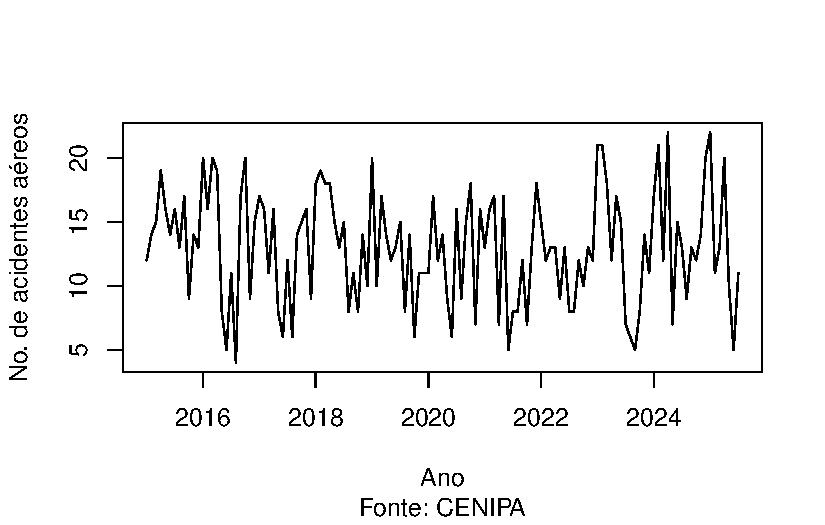
\includegraphics{polinomial_files/figure-pdf/unnamed-chunk-18-1.pdf}

}

\end{figure}

\begin{Shaded}
\begin{Highlighting}[]
\FunctionTok{acf}\NormalTok{(erros)}
\end{Highlighting}
\end{Shaded}

\begin{figure}[H]

{\centering 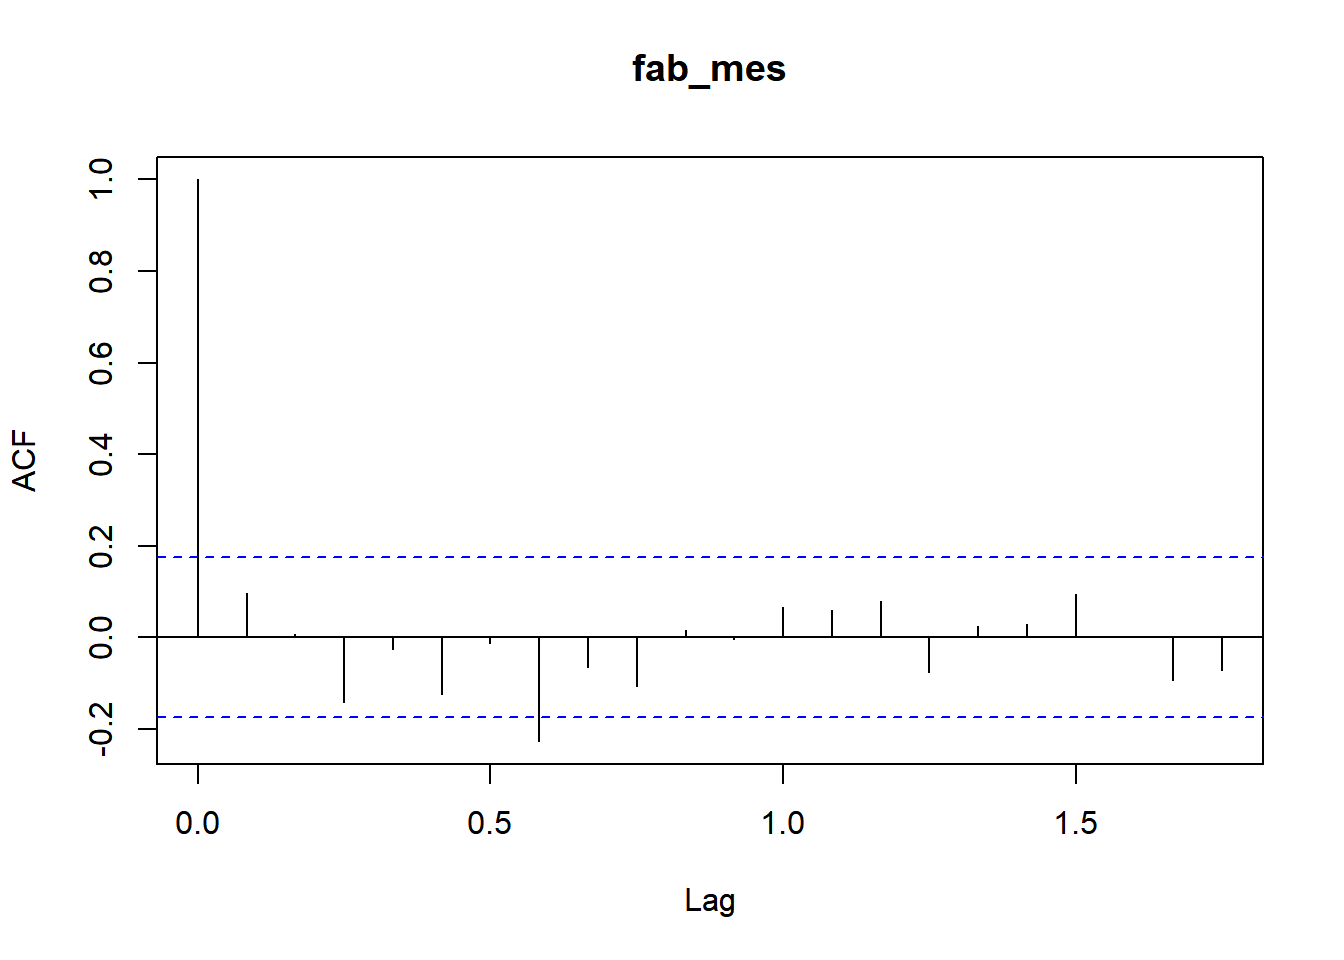
\includegraphics{polinomial_files/figure-pdf/unnamed-chunk-18-2.pdf}

}

\end{figure}

Ambos os gráficos acima mostram um comportamento de ruído branco.

Podemos fazer previsões mais longas com este modelo. Abaixo vamos prever
o número de acidentes para os próximos 12 meses.

\begin{Shaded}
\begin{Highlighting}[]
\NormalTok{previsao12 }\OtherTok{\textless{}{-}} \FunctionTok{dlmForecast}\NormalTok{(filtro,}\DecValTok{12}\NormalTok{)}
\NormalTok{previsao12}\SpecialCharTok{$}\NormalTok{f}
\end{Highlighting}
\end{Shaded}

\begin{verbatim}
          Jan      Feb      Mar      Apr      May      Jun      Jul      Aug
2023                                                       51.74024 51.79805
2024 52.08715 52.14496 52.20278 52.26060 52.31842 52.37624                  
          Sep      Oct      Nov      Dec
2023 51.85587 51.91369 51.97151 52.02933
2024                                    
\end{verbatim}

Vamos colocar essas informações em um gráfico. Vamos começar com as
previsões um passo a frente, que são utilizadas para o cálculo do erro
de previsão e queforam realizadas dentro do filtro de Kalman - notem que
vamos começar as previsões em março, uma vez que as outras foram
irreais). Em seguida, vamos apresentar as previsões com um intervalo de
90\% de predição (não se usa 95\% para previsões porque os intervalos em
geral são grandes demais)

\begin{Shaded}
\begin{Highlighting}[]
\FunctionTok{ts.plot}\NormalTok{(fab\_mes,}\AttributeTok{xlim=}\FunctionTok{c}\NormalTok{(}\DecValTok{2013}\NormalTok{,}\DecValTok{2025}\NormalTok{), }\AttributeTok{ylab=}\StringTok{\textquotesingle{}No. acidentes mensais\textquotesingle{}}\NormalTok{, }\AttributeTok{ylim=}\FunctionTok{c}\NormalTok{(}\DecValTok{0}\NormalTok{,}\DecValTok{75}\NormalTok{))}
\FunctionTok{lines}\NormalTok{( }\FunctionTok{window}\NormalTok{(filtro}\SpecialCharTok{$}\NormalTok{f,}\AttributeTok{start=}\FunctionTok{c}\NormalTok{(}\DecValTok{2013}\NormalTok{,}\DecValTok{3}\NormalTok{)), }\AttributeTok{lty=}\DecValTok{2}\NormalTok{,}\AttributeTok{lwd =} \DecValTok{2}\NormalTok{)}

\CommentTok{\# medidas para o intervalo de previsão}
\NormalTok{media\_prev }\OtherTok{\textless{}{-}}\NormalTok{ previsao12}\SpecialCharTok{$}\NormalTok{f}
\NormalTok{media\_prev }\OtherTok{\textless{}{-}} \FunctionTok{ts}\NormalTok{(media\_prev, }\AttributeTok{start =} \FunctionTok{c}\NormalTok{(}\DecValTok{2023}\NormalTok{,}\DecValTok{7}\NormalTok{), }\AttributeTok{frequency =} \DecValTok{12}\NormalTok{)}

\NormalTok{desv\_prev }\OtherTok{\textless{}{-}} \FunctionTok{sqrt}\NormalTok{( }\FunctionTok{unlist}\NormalTok{( previsao12}\SpecialCharTok{$}\NormalTok{Q))}
\NormalTok{desv\_prev }\OtherTok{\textless{}{-}} \FunctionTok{ts}\NormalTok{(desv\_prev, }\AttributeTok{start =} \FunctionTok{c}\NormalTok{(}\DecValTok{2023}\NormalTok{,}\DecValTok{7}\NormalTok{), }\AttributeTok{frequency =} \DecValTok{12}\NormalTok{)}

\CommentTok{\# intervalo de 90\% para as previsões}
\FunctionTok{lines}\NormalTok{(media\_prev, }\AttributeTok{lwd =} \DecValTok{2}\NormalTok{, }\AttributeTok{col =}\StringTok{\textquotesingle{}blue\textquotesingle{}}\NormalTok{)}
\FunctionTok{lines}\NormalTok{(media\_prev }\SpecialCharTok{{-}}\FloatTok{1.64}\SpecialCharTok{*}\NormalTok{desv\_prev, }\AttributeTok{lwd =} \DecValTok{2}\NormalTok{, }\AttributeTok{col =}\StringTok{\textquotesingle{}blue\textquotesingle{}}\NormalTok{)}
\FunctionTok{lines}\NormalTok{(media\_prev}\FloatTok{+1.64}\SpecialCharTok{*}\NormalTok{desv\_prev, }\AttributeTok{lwd =} \DecValTok{2}\NormalTok{, }\AttributeTok{col =}\StringTok{\textquotesingle{}blue\textquotesingle{}}\NormalTok{)}

\CommentTok{\# legenda}
\FunctionTok{legend}\NormalTok{(}\StringTok{\textquotesingle{}bottomleft\textquotesingle{}}\NormalTok{,}\FunctionTok{c}\NormalTok{(}\StringTok{\textquotesingle{}Série observada\textquotesingle{}}\NormalTok{,}\StringTok{\textquotesingle{}Previsão 1 passo à frente\textquotesingle{}}\NormalTok{, }\StringTok{\textquotesingle{}Previsão de 12 meses\textquotesingle{}}\NormalTok{), }\AttributeTok{lty=}\FunctionTok{c}\NormalTok{(}\DecValTok{1}\NormalTok{,}\DecValTok{2}\NormalTok{,}\DecValTok{1}\NormalTok{), }\AttributeTok{col =}\FunctionTok{c}\NormalTok{(}\DecValTok{1}\NormalTok{,}\DecValTok{1}\NormalTok{,}\StringTok{\textquotesingle{}blue\textquotesingle{}}\NormalTok{), }\AttributeTok{bty =} \StringTok{\textquotesingle{}n\textquotesingle{}}\NormalTok{)}
\end{Highlighting}
\end{Shaded}

\begin{figure}[H]

{\centering 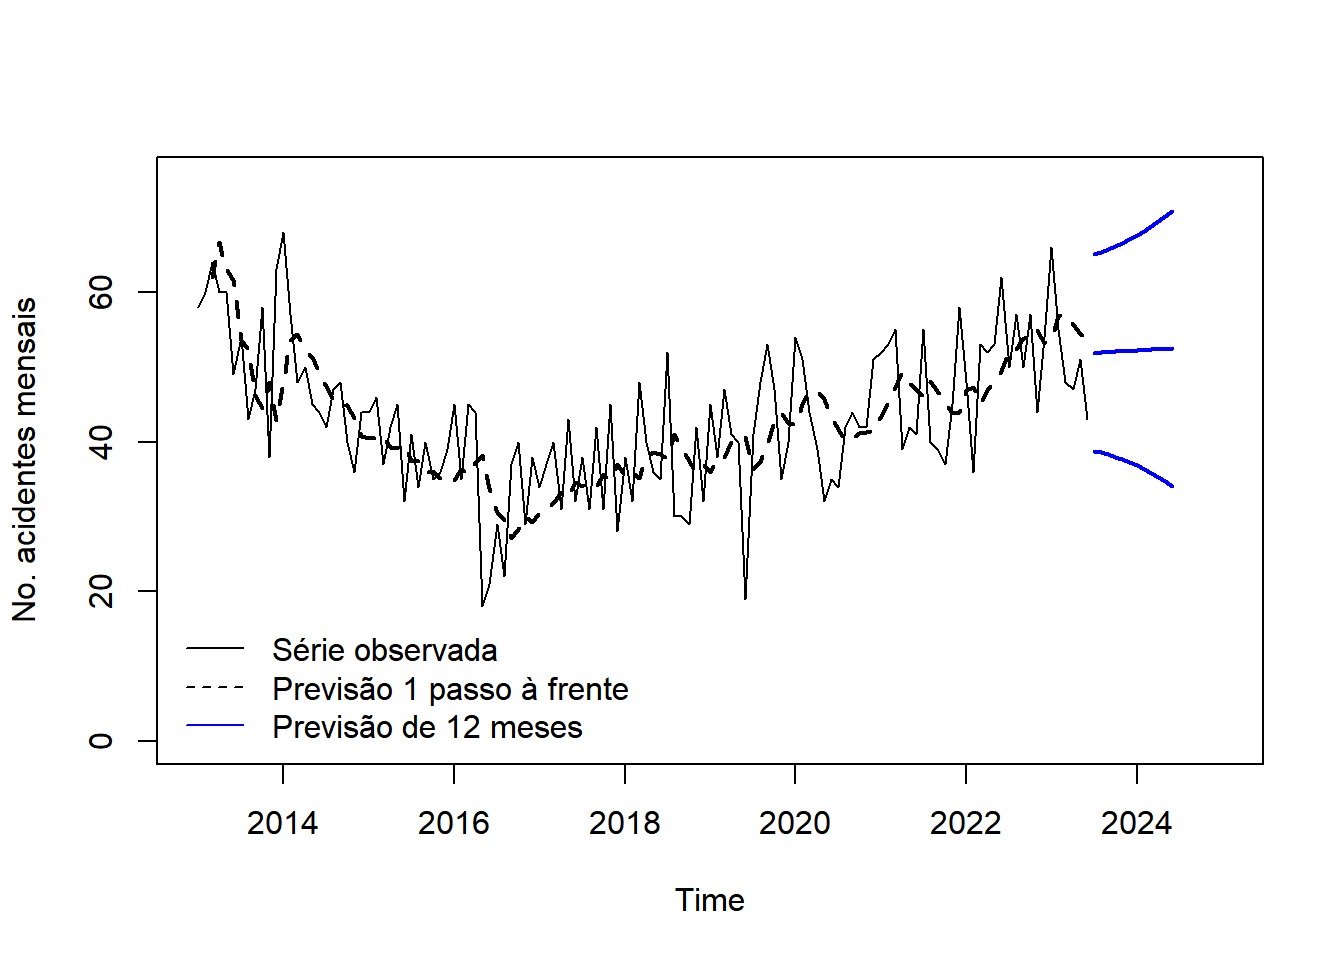
\includegraphics{polinomial_files/figure-pdf/unnamed-chunk-20-1.pdf}

}

\end{figure}

Agora vamos estudar os estados suavizados. `

\begin{Shaded}
\begin{Highlighting}[]
\NormalTok{suave }\OtherTok{\textless{}{-}} \FunctionTok{dlmSmooth}\NormalTok{(filtro)}
\end{Highlighting}
\end{Shaded}

A obtenção das variâncias é mais delicada. Em cada instante de tempo, é
calculada a matriz

\[S_t=\left( \begin{array}{cc} s_{11,t} & s_{12,t}\\s_{12,t}&s_{22,t}\end{array}\right),\]
que reprenta em sua diagonal a variância dos estados e fora dela a
covariância entre eles. Por motivos computacionais, a matriz \(S_t\) não
é computada diretamente, mas sim duas matrizes \(U_t\) e \(D_t\) tais
que

\[S_t=U_t D_t U_t'\] Essa decomposição, conhecida como espectral, possui
vantagens numéricas que facilitam o processo de inversão necessário no
filtro de Kalman. A função abaixo recupera o desvio padrão a partir de
\(U_t\) e \(D_t\).

\begin{Shaded}
\begin{Highlighting}[]
\NormalTok{sdSmooth }\OtherTok{\textless{}{-}} \ControlFlowTok{function}\NormalTok{(suave)\{}
\NormalTok{  n }\OtherTok{\textless{}{-}} \FunctionTok{nrow}\NormalTok{(suave}\SpecialCharTok{$}\NormalTok{s)}
\NormalTok{  q }\OtherTok{\textless{}{-}} \FunctionTok{ncol}\NormalTok{(suave}\SpecialCharTok{$}\NormalTok{s)}
\NormalTok{  dp }\OtherTok{\textless{}{-}} \FunctionTok{array}\NormalTok{(}\ConstantTok{NA\_real\_}\NormalTok{, }\FunctionTok{c}\NormalTok{( n , q))}
  \ControlFlowTok{for}\NormalTok{(i }\ControlFlowTok{in} \DecValTok{1}\SpecialCharTok{:}\NormalTok{n)\{}
\NormalTok{    S }\OtherTok{\textless{}{-}} \FunctionTok{dlmSvd2var}\NormalTok{(suave}\SpecialCharTok{$}\NormalTok{U.S[[i]],suave}\SpecialCharTok{$}\NormalTok{D.S[i,])}
\NormalTok{    dp[i,] }\OtherTok{\textless{}{-}} \FunctionTok{sqrt}\NormalTok{( }\FunctionTok{diag}\NormalTok{(S))}
\NormalTok{  \}}
\NormalTok{  dp}
\NormalTok{\}}
\end{Highlighting}
\end{Shaded}

Abaixo, vamos obter os desvios da suavização

\begin{Shaded}
\begin{Highlighting}[]
\NormalTok{sd }\OtherTok{\textless{}{-}} \FunctionTok{sdSmooth}\NormalTok{(suave)}
\end{Highlighting}
\end{Shaded}

Vamos começar a análise com o nível. Observe que, como são 2 estados,
devemos selecionar a coluna 1.

\begin{Shaded}
\begin{Highlighting}[]
\NormalTok{nivel\_medio }\OtherTok{\textless{}{-}}\NormalTok{ suave}\SpecialCharTok{$}\NormalTok{s[,}\DecValTok{1}\NormalTok{]}
\NormalTok{sd\_nivel }\OtherTok{\textless{}{-}}\NormalTok{ sd[,}\DecValTok{1}\NormalTok{]}

\FunctionTok{ts.plot}\NormalTok{(fab\_mes)}
\FunctionTok{lines}\NormalTok{(nivel\_medio, }\AttributeTok{lwd =} \DecValTok{2}\NormalTok{, }\AttributeTok{col =} \StringTok{\textquotesingle{}seagreen\textquotesingle{}}\NormalTok{)}

\CommentTok{\# intervalor de credibilidade (95\%) para o nível}
\FunctionTok{lines}\NormalTok{(nivel\_medio }\SpecialCharTok{{-}} \FloatTok{1.96}\SpecialCharTok{*}\NormalTok{sd\_nivel, }\AttributeTok{lwd =} \DecValTok{2}\NormalTok{, }\AttributeTok{col =} \StringTok{\textquotesingle{}seagreen\textquotesingle{}}\NormalTok{, }\AttributeTok{lty=} \DecValTok{2}\NormalTok{)}
\FunctionTok{lines}\NormalTok{(nivel\_medio }\SpecialCharTok{+} \FloatTok{1.96}\SpecialCharTok{*}\NormalTok{sd\_nivel, }\AttributeTok{lwd =} \DecValTok{2}\NormalTok{, }\AttributeTok{col =} \StringTok{\textquotesingle{}seagreen\textquotesingle{}}\NormalTok{, }\AttributeTok{lty=}\DecValTok{2}\NormalTok{)}
\end{Highlighting}
\end{Shaded}

\begin{figure}[H]

{\centering \includegraphics{polinomial_files/figure-pdf/unnamed-chunk-24-1.pdf}

}

\end{figure}

Por último, vamos analisar a inclinação da tendência. Como a média da
série já foi modelada pelo nível, os gráficos das demais componentes não
são colocados sobre a série original. Abaixo mostramos o gráfico da
inclinação, com seu respectivo intervalo.

\begin{Shaded}
\begin{Highlighting}[]
\NormalTok{tend }\OtherTok{\textless{}{-}}\NormalTok{ suave}\SpecialCharTok{$}\NormalTok{s[,}\DecValTok{2}\NormalTok{]}
\NormalTok{sd\_tend }\OtherTok{\textless{}{-}}\NormalTok{ sd[,}\DecValTok{2}\NormalTok{]}
\FunctionTok{ts.plot}\NormalTok{(tend, }\AttributeTok{lwd =} \DecValTok{2}\NormalTok{, }\AttributeTok{ylim=}\FunctionTok{c}\NormalTok{(}\SpecialCharTok{{-}}\FloatTok{1.5}\NormalTok{,}\DecValTok{1}\NormalTok{), }\AttributeTok{ylab=}\StringTok{\textquotesingle{}Inclinação da tendência\textquotesingle{}}\NormalTok{)}
\FunctionTok{lines}\NormalTok{(tend}\FloatTok{{-}1.96}\SpecialCharTok{*}\NormalTok{sd\_tend)}
\FunctionTok{lines}\NormalTok{(tend}\FloatTok{+1.96}\SpecialCharTok{*}\NormalTok{sd\_tend)}
\FunctionTok{abline}\NormalTok{(}\AttributeTok{h=}\DecValTok{0}\NormalTok{, }\AttributeTok{lty =} \DecValTok{2}\NormalTok{)}

\CommentTok{\# período de mudança da tendência de decrescente para crescente}
\FunctionTok{abline}\NormalTok{(}\AttributeTok{v=}\DecValTok{2016}\SpecialCharTok{+}\DecValTok{10}\SpecialCharTok{/}\DecValTok{12}\NormalTok{, }\AttributeTok{lty =} \DecValTok{2}\NormalTok{)}
\FunctionTok{points}\NormalTok{(}\DecValTok{2016}\SpecialCharTok{+}\DecValTok{10}\SpecialCharTok{/}\DecValTok{12}\NormalTok{,}\DecValTok{0}\NormalTok{, }\AttributeTok{pch =} \DecValTok{15}\NormalTok{, }\AttributeTok{cex =} \FloatTok{1.2}\NormalTok{)}
\FunctionTok{text}\NormalTok{(}\DecValTok{2016}\SpecialCharTok{+}\DecValTok{11}\SpecialCharTok{/}\DecValTok{12}\NormalTok{,.}\DecValTok{1}\NormalTok{,}\StringTok{\textquotesingle{}Oct 16\textquotesingle{}}\NormalTok{, }\AttributeTok{pos =} \DecValTok{2}\NormalTok{)}

\CommentTok{\# identificando a desaceleração}
\NormalTok{x }\OtherTok{\textless{}{-}} \FunctionTok{window}\NormalTok{(tend, }\AttributeTok{start=}\FunctionTok{c}\NormalTok{(}\DecValTok{2022}\NormalTok{,}\DecValTok{7}\NormalTok{) )}
\FunctionTok{abline}\NormalTok{(}\AttributeTok{v=}\DecValTok{2022}\SpecialCharTok{+}\DecValTok{7}\SpecialCharTok{/}\DecValTok{12}\NormalTok{, }\AttributeTok{lty =} \DecValTok{2}\NormalTok{)}
\FunctionTok{points}\NormalTok{(}\DecValTok{2022}\SpecialCharTok{+}\DecValTok{7}\SpecialCharTok{/}\DecValTok{12}\NormalTok{, x[}\DecValTok{1}\NormalTok{], }\AttributeTok{pch =} \DecValTok{15}\NormalTok{, }\AttributeTok{cex =} \FloatTok{1.2}\NormalTok{)}
\FunctionTok{text}\NormalTok{(}\DecValTok{2022}\SpecialCharTok{+}\DecValTok{7}\SpecialCharTok{/}\DecValTok{12}\NormalTok{,x[}\DecValTok{1}\NormalTok{],}\StringTok{\textquotesingle{}Jul 22\textquotesingle{}}\NormalTok{, }\AttributeTok{pos =} \DecValTok{2}\NormalTok{)}
\end{Highlighting}
\end{Shaded}

\begin{figure}[H]

{\centering \includegraphics{polinomial_files/figure-pdf/unnamed-chunk-25-1.pdf}

}

\end{figure}

Com o gráfico acima, identificamos muitas características interessantes.

\begin{itemize}
\item
  Note que o zero está presente na maior parte do intervalo. Portanto,
  podemos apenas afirmar que em certos períodos, a tendência de
  crescimento/decrescimento foram mais prováveis.
\item
  Em relação à inclinação média, podemos afirmar que existem evidências
  de que o padrão de decrescimento estava desacelerando antes de 2016,
  culminando na inflexão em outubro. Nesse período a série passou a ter
  uma taxa de crescimento relativamente constante até Julho de 2022,
  quando começou a desacelar.
\end{itemize}

\hypertarget{exercuxedcios-4}{%
\section{Exercícios}\label{exercuxedcios-4}}

Abaixo, mostramos o número de homicídios mensais em Manaus entre Janeiro
de 1979 e Dezembro de 2009.

\begin{Shaded}
\begin{Highlighting}[]
\NormalTok{url }\OtherTok{\textless{}{-}} \StringTok{\textquotesingle{}https://www.dropbox.com/s/hcqq6uhgwnimpcn/homicidios\_manaus\_SIM.csv?dl=1\textquotesingle{}}
\end{Highlighting}
\end{Shaded}

\begin{itemize}
\item
  Explore a série.
\item
  Estude o nível da série
\item
  Estude o comportamento da inclinação, identificando possíveis regimes
  de aceleração/desaceleração de crescimento.
\end{itemize}

Analise a série de suicídios no Mato Grosso do Sul, estudando o nível da
série e a inclinação da tendência.

\begin{Shaded}
\begin{Highlighting}[]
\NormalTok{url }\OtherTok{\textless{}{-}} \StringTok{\textquotesingle{}https://drive.google.com/uc?authuser=0\&id=1DMSgrQDl0636Lw0Y0MYJHJrgw\_2uXntM\&export=download\textquotesingle{}}
\end{Highlighting}
\end{Shaded}

\bookmarksetup{startatroot}

\hypertarget{modelos-lineares-dinuxe2micos-sazonais}{%
\chapter{Modelos lineares dinâmicos
sazonais}\label{modelos-lineares-dinuxe2micos-sazonais}}

\begin{verbatim}
Carregando pacotes exigidos: dlm
\end{verbatim}

\begin{verbatim}
Warning: package 'dlm' was built under R version 4.3.1
\end{verbatim}

\hypertarget{a-soma-de-um-ciclo-sazonal}{%
\section{A soma de um ciclo sazonal}\label{a-soma-de-um-ciclo-sazonal}}

Como ilustração, considere um efeito sazonal trimestral (período 4).
Considere os seguintes fatores sazonais:

\[\beta_t=\left\{\begin{array}{ll}1,& t=1,5,9,\ldots \\
2,& t=2,6,10,\ldots\\
3,&t=3,7,11,\ldots \\
4,&t=4,8,12,\ldots\end{array}\right.\]

Note que \[\beta_1+\beta_2+\beta_3+\beta_4=10\]

Também note que \[\beta_2+\beta_3+\beta_4+\beta_5=10\] e que o mesmo é
verdade para a soma de 4 quaiquer fatores sazonais consecutivos. Pode-se
provar que, para qualquer sinal sazonal, a soma de seu efeito
considerando um intervalo de tempo igual ao período é constante.

Considere então que uma série com período 4, fatores sazonais
desconhecidos e e uma uma tendência, do tipo
\[\hbox{tendência}(t)=\alpha+\gamma t.\] Então, para qualquer
\(k=0,1,2,\ldots,\)

\[y_{k+1}+y_{k+2}+y_{k+3}+y_{k+4}=4\alpha+\gamma(10+4k)+\beta_1+\beta_2+\beta_3+\beta_4\]

Portanto, se os dados forem agregados para construir uma série anual, é
impossível estimar \(\alpha\) e \(\beta_1+\beta_2+\beta_3+\beta_4\) em
separado. Por isso, assuminos que a soma dos fatores sazonais deve ser
nula. Intuitivamente, estamos dizendo que o nível da série não pode ser
modelado pela tendência.

\hypertarget{o-modelo-linear-dinuxe2mico-para-fatores-sazonais}{%
\section{O modelo linear dinâmico para fatores
sazonais}\label{o-modelo-linear-dinuxe2mico-para-fatores-sazonais}}

Considere uma série sazonal com período \(p\). No modelo linear dinâmico
para fatores sazonais, assumimos que existem \(p-1\) fatores sazonais,

\[\psi_1,\ldots,\psi_{p-1},\] sendo que o \(p\)-ésimo fator é,
necessariamente \(-(\psi_1-\psi_2-\cdots-\psi_{p-1}\). Além disso,
permitimos que cada fator evolua no tempo, o que implica na notação
\(\psi_t\). Contudo, neste modelo consideramos apenas uma evolução de
nível para os fatores (em um problema mensal, todos os janeiros estariam
flutuando em torno de um nível, por exemplo). Por este motivo, a
previsão para cada fator dentro dentro de uma determinada posição do
ciclo sazonal será constante.

A função \texttt{dlmModSeas} constrói as matrizes \(F_t\) e \(G_t\) para
o modelo com fatores sazonais dinâmicos. Vamos ilustrar o uso deste
modelo utilizando a série \texttt{nottem} - por didática, vamos remover
a tendência da série via \texttt{loess}.

\begin{Shaded}
\begin{Highlighting}[]
\NormalTok{tempo }\OtherTok{\textless{}{-}} \DecValTok{1}\SpecialCharTok{:}\FunctionTok{length}\NormalTok{(nottem)}
\NormalTok{dnottem }\OtherTok{\textless{}{-}}\NormalTok{ nottem }\SpecialCharTok{{-}} \FunctionTok{loess}\NormalTok{( nottem }\SpecialCharTok{\textasciitilde{}}\NormalTok{ tempo)}\SpecialCharTok{$}\NormalTok{fit}
\FunctionTok{ts.plot}\NormalTok{(dnottem)}
\FunctionTok{abline}\NormalTok{(}\AttributeTok{h=}\DecValTok{0}\NormalTok{,}\AttributeTok{lty =}\DecValTok{2}\NormalTok{)}
\end{Highlighting}
\end{Shaded}

\begin{figure}[H]

{\centering \includegraphics{sazonal_files/figure-pdf/unnamed-chunk-2-1.pdf}

}

\end{figure}

Já identificamos, em outro momento, que o período desta série é 12, logo

\begin{Shaded}
\begin{Highlighting}[]
\NormalTok{mod }\OtherTok{\textless{}{-}} \FunctionTok{dlmModSeas}\NormalTok{(}\DecValTok{12}\NormalTok{)}
\end{Highlighting}
\end{Shaded}

Precisamos colocar uma informação sobre os fatores sazonais. Vamos
simplesmente assumir que todos valem zero.

\begin{Shaded}
\begin{Highlighting}[]
\NormalTok{mod}\SpecialCharTok{$}\NormalTok{m0 }\OtherTok{\textless{}{-}} \FunctionTok{rep}\NormalTok{(}\DecValTok{0}\NormalTok{,}\DecValTok{11}\NormalTok{)}
\end{Highlighting}
\end{Shaded}

Vamos estimar as variâncias:

\begin{Shaded}
\begin{Highlighting}[]
\NormalTok{mod }\OtherTok{\textless{}{-}} \FunctionTok{modFim}\NormalTok{(dnottem, mod)}
\end{Highlighting}
\end{Shaded}

Em seguida, aplicamos o filtro de Kalman e verificamos os erros de
previsão:

\begin{Shaded}
\begin{Highlighting}[]
\NormalTok{filtro }\OtherTok{\textless{}{-}} \FunctionTok{dlmFilter}\NormalTok{(dnottem, mod)}

\NormalTok{erro }\OtherTok{\textless{}{-}}\NormalTok{ dnottem }\SpecialCharTok{{-}}\NormalTok{ filtro}\SpecialCharTok{$}\NormalTok{f}
\FunctionTok{ts.plot}\NormalTok{(erro)}
\end{Highlighting}
\end{Shaded}

\begin{figure}[H]

{\centering \includegraphics{sazonal_files/figure-pdf/unnamed-chunk-6-1.pdf}

}

\end{figure}

\begin{Shaded}
\begin{Highlighting}[]
\FunctionTok{acf}\NormalTok{(erro)}
\end{Highlighting}
\end{Shaded}

\begin{figure}[H]

{\centering \includegraphics{sazonal_files/figure-pdf/unnamed-chunk-6-2.pdf}

}

\end{figure}

Podemos notar que os erros foram altos no começo da série. Em geral,
precisamos de pelos menos dois ciclos sazonais para ter uma previsão
melhor. Já no correlograma, sobraram alguns elementos para serem
explicados, como uma relação da série com as defasagens 1 e 2 e uma
sazonalidade autoregressiva. Contudo, o comportamento sazonal, que era
nosso objetivo, foi bem explicado.

As previsões vão se repetir após \(12\) unidades de tempo. Abaixo,
fazemos a previsão para 2 anos.

\begin{Shaded}
\begin{Highlighting}[]
\NormalTok{previsao24 }\OtherTok{\textless{}{-}} \FunctionTok{dlmForecast}\NormalTok{(filtro,}\DecValTok{24}\NormalTok{)}
\NormalTok{previsao24}\SpecialCharTok{$}\NormalTok{f}
\end{Highlighting}
\end{Shaded}

\begin{verbatim}
             Jan         Feb         Mar         Apr         May         Jun
1940  -9.5090113  -9.3187060  -6.4630679  -2.5432743   3.0899591   9.1372660
1941  -9.5090113  -9.3187060  -6.4630679  -2.5432743   3.0899591   9.1372660
             Jul         Aug         Sep         Oct         Nov         Dec
1940  11.6220692  11.9971484   7.9912336  -0.5276387  -4.5933683 -10.8826097
1941  11.6220692  11.9971484   7.9912336  -0.5276387  -4.5933683 -10.8826097
\end{verbatim}

Vamos colocar essas informações em um gráfico.

\begin{Shaded}
\begin{Highlighting}[]
\FunctionTok{ts.plot}\NormalTok{(dnottem,}\AttributeTok{xlim=}\FunctionTok{c}\NormalTok{(}\DecValTok{1920}\NormalTok{,}\DecValTok{1942}\NormalTok{), }\AttributeTok{ylim=}\FunctionTok{c}\NormalTok{(}\SpecialCharTok{{-}}\DecValTok{20}\NormalTok{,}\DecValTok{20}\NormalTok{))}
\FunctionTok{lines}\NormalTok{( }\FunctionTok{window}\NormalTok{(filtro}\SpecialCharTok{$}\NormalTok{f,}\AttributeTok{start=}\FunctionTok{c}\NormalTok{(}\DecValTok{1920}\NormalTok{,}\DecValTok{12}\NormalTok{)), }\AttributeTok{lty=}\DecValTok{2}\NormalTok{,}\AttributeTok{lwd =} \DecValTok{2}\NormalTok{)}

\CommentTok{\# medidas para o intervalo de previsão}
\NormalTok{media\_prev }\OtherTok{\textless{}{-}}\NormalTok{ previsao24}\SpecialCharTok{$}\NormalTok{f}
\NormalTok{media\_prev }\OtherTok{\textless{}{-}} \FunctionTok{ts}\NormalTok{(media\_prev, }\AttributeTok{start =} \FunctionTok{c}\NormalTok{(}\DecValTok{1940}\NormalTok{,}\DecValTok{1}\NormalTok{), }\AttributeTok{frequency =} \DecValTok{12}\NormalTok{)}

\NormalTok{desv\_prev }\OtherTok{\textless{}{-}} \FunctionTok{sqrt}\NormalTok{( }\FunctionTok{unlist}\NormalTok{( previsao24}\SpecialCharTok{$}\NormalTok{Q))}
\NormalTok{desv\_prev }\OtherTok{\textless{}{-}} \FunctionTok{ts}\NormalTok{(desv\_prev, }\AttributeTok{start =} \FunctionTok{c}\NormalTok{(}\DecValTok{1940}\NormalTok{,}\DecValTok{1}\NormalTok{), }\AttributeTok{frequency =} \DecValTok{12}\NormalTok{)}

\CommentTok{\# intervalo de 90\% para as previsões}
\FunctionTok{lines}\NormalTok{(media\_prev, }\AttributeTok{lwd =} \DecValTok{2}\NormalTok{, }\AttributeTok{col =}\StringTok{\textquotesingle{}blue\textquotesingle{}}\NormalTok{)}
\FunctionTok{lines}\NormalTok{(media\_prev }\SpecialCharTok{{-}}\FloatTok{1.64}\SpecialCharTok{*}\NormalTok{desv\_prev, }\AttributeTok{lwd =} \DecValTok{2}\NormalTok{, }\AttributeTok{col =}\StringTok{\textquotesingle{}blue\textquotesingle{}}\NormalTok{)}
\FunctionTok{lines}\NormalTok{(media\_prev}\FloatTok{+1.64}\SpecialCharTok{*}\NormalTok{desv\_prev, }\AttributeTok{lwd =} \DecValTok{2}\NormalTok{, }\AttributeTok{col =}\StringTok{\textquotesingle{}blue\textquotesingle{}}\NormalTok{)}

\CommentTok{\# legenda}
\FunctionTok{legend}\NormalTok{(}\StringTok{\textquotesingle{}bottomleft\textquotesingle{}}\NormalTok{,}\FunctionTok{c}\NormalTok{(}\StringTok{\textquotesingle{}Série observada\textquotesingle{}}\NormalTok{,}\StringTok{\textquotesingle{}Previsão 1 passo à frente\textquotesingle{}}\NormalTok{, }\StringTok{\textquotesingle{}Previsão de 24 meses\textquotesingle{}}\NormalTok{), }\AttributeTok{lty=}\FunctionTok{c}\NormalTok{(}\DecValTok{1}\NormalTok{,}\DecValTok{2}\NormalTok{,}\DecValTok{1}\NormalTok{), }\AttributeTok{col =}\FunctionTok{c}\NormalTok{(}\DecValTok{1}\NormalTok{,}\DecValTok{1}\NormalTok{,}\StringTok{\textquotesingle{}blue\textquotesingle{}}\NormalTok{), }\AttributeTok{bty =} \StringTok{\textquotesingle{}n\textquotesingle{}}\NormalTok{)}
\end{Highlighting}
\end{Shaded}

\begin{figure}[H]

{\centering \includegraphics{sazonal_files/figure-pdf/unnamed-chunk-8-1.pdf}

}

\end{figure}

Agora vamos estudar os estados suavizados. `

\begin{Shaded}
\begin{Highlighting}[]
\NormalTok{suave }\OtherTok{\textless{}{-}} \FunctionTok{dlmSmooth}\NormalTok{(filtro)}
\NormalTok{sd }\OtherTok{\textless{}{-}} \FunctionTok{sdSmooth}\NormalTok{(suave)}
\end{Highlighting}
\end{Shaded}

Como o período é 12, existem \(p-1=11\) estados nesse modelo. Contudo, a
matriz \(G_t\) é construída de modo que o primeiro estado sempre contém
o fator sazonal da vez. Portanto, para poder analizar os fatores
sazonais suavizados, basta selecionar a primeira coluna de \texttt{s}
dentro do objeto \texttt{suave}

\begin{Shaded}
\begin{Highlighting}[]
\NormalTok{nivel\_medio }\OtherTok{\textless{}{-}}\NormalTok{ suave}\SpecialCharTok{$}\NormalTok{s[,}\DecValTok{1}\NormalTok{]}
\NormalTok{sd\_nivel }\OtherTok{\textless{}{-}}\NormalTok{ sd[,}\DecValTok{1}\NormalTok{]}

\FunctionTok{ts.plot}\NormalTok{(dnottem)}
\FunctionTok{lines}\NormalTok{(nivel\_medio, }\AttributeTok{lwd =} \DecValTok{2}\NormalTok{, }\AttributeTok{col =} \StringTok{\textquotesingle{}seagreen\textquotesingle{}}\NormalTok{)}

\CommentTok{\# intervalor de credibilidade (95\%) para o nível}
\FunctionTok{lines}\NormalTok{(nivel\_medio }\SpecialCharTok{{-}} \FloatTok{1.96}\SpecialCharTok{*}\NormalTok{sd\_nivel, }\AttributeTok{lwd =} \DecValTok{2}\NormalTok{, }\AttributeTok{col =} \StringTok{\textquotesingle{}seagreen\textquotesingle{}}\NormalTok{, }\AttributeTok{lty=} \DecValTok{2}\NormalTok{)}
\FunctionTok{lines}\NormalTok{(nivel\_medio }\SpecialCharTok{+} \FloatTok{1.96}\SpecialCharTok{*}\NormalTok{sd\_nivel, }\AttributeTok{lwd =} \DecValTok{2}\NormalTok{, }\AttributeTok{col =} \StringTok{\textquotesingle{}seagreen\textquotesingle{}}\NormalTok{, }\AttributeTok{lty=}\DecValTok{2}\NormalTok{)}
\end{Highlighting}
\end{Shaded}

\begin{figure}[H]

{\centering \includegraphics{sazonal_files/figure-pdf/unnamed-chunk-10-1.pdf}

}

\end{figure}

\hypertarget{regressuxe3o-harmuxf4nica-dinuxe2mica}{%
\section{Regressão harmônica
dinâmica}\label{regressuxe3o-harmuxf4nica-dinuxe2mica}}

Vimos anteriormente que uma onda, de período \(p\), pode ser
representada pela função harmônica

\[g_1(t)=A_1\cos\left(\frac{2\pi}{p}t+\phi_1\right).\] Acontece que é
possível que existam outros ciclos dentro do de duração \(p\).

Para ilustrar, vamos imaginar o caso no qual \(p=12\). Então, temos uma
onda se reinicia a cada \(12\) meses, isto é,

\[g_1(t)=A_1\cos\left(\frac{2\pi}{12}t+\phi_1\right).\] Acontece que é
possível que existam Porém podemos ter um outro efeito, que se renova a
cada semestre. Nesse caso, teríamos outro harmônico para esse
comportamento

\[g_2(t)=A_2\cos\left(\frac{2\pi}{6}t+\phi_2\right)\]

Também podemos ter um ciclo se repetindo a cada quatrimestre

\[g_3(t)=A_3\cos\left(\frac{2\pi}{4}t+\phi_3\right),\] e outro a cada
trimestre

\[g_4(t)=A_4\cos\left(\frac{2\pi}{3}t+\phi_4\right).\]

Então, o nosso padrão sazonal seria a soma desses harmônicos:

\[g(t)=\sum_{j=1}^4 g_{j}(t)=\sum_{j=1}^4 A_j\cos\left(\frac{2\pi}{p}jt+\phi_j\right).\]
A função \(g_j(t)\) é denominada \(j\)-ésimo harmônico e é possível ter
\(q\) harmônicos, onde \(q\) é a parte inteira de \(p/2\).

A figura abaixo ilustra essa ideia.

\includegraphics{sazonal_files/figure-pdf/unnamed-chunk-11-1.pdf}

No caso geral, para um período \(p\), podemos converter o modelo acima
em um modelo linear

\[g(t)=\sum_{j=1}^{q} \beta_{1,j}\cos\left(\frac{2\pi}{p}jt\right)+\beta_{2,j}\sin\left(\frac{2\pi}{p}jt\right).\]
De fato, existe \(\boldsymbol{F}_t'\) tal que

\[g(t)=\boldsymbol{F}_t'\boldsymbol{\beta},\] onde
\(\boldsymbol{\beta}\) é um vetor contendo
\(\beta_{1,1},\beta_{1,2},\ldots,\beta_{1,q},\beta_{2,q}\). O modelo

\[y_t= \boldsymbol{F}_t'\boldsymbol{\beta}+\varepsilon_t\] é denominado
regressão harmônica. Assumindo que o vetor de parâmetros pode evoluir no
tempo \(t\), considerando uma estrutura de nível, teremos o modelo de
regressão harmônica dinâmico.

Vamos analisar a série \texttt{dnottem} utilizando esse modelo com
apenas um harmônico. A função \texttt{dlmModTrig(p,q)} cria as matrizes
necessárias para o modelo de regressão harmônica com período \(p\) e
\(q\) harmônicos (se omitido, serão utilizados \(p/2\) harmônicos).

\begin{Shaded}
\begin{Highlighting}[]
\NormalTok{mod }\OtherTok{\textless{}{-}} \FunctionTok{dlmModTrig}\NormalTok{(}\DecValTok{12}\NormalTok{, }\DecValTok{1}\NormalTok{)}
\NormalTok{mod }\OtherTok{\textless{}{-}} \FunctionTok{modFim}\NormalTok{( dnottem, mod)}
\end{Highlighting}
\end{Shaded}

Vamos aplicar o filtro de Kalman:

\begin{Shaded}
\begin{Highlighting}[]
\NormalTok{filtro }\OtherTok{\textless{}{-}} \FunctionTok{dlmFilter}\NormalTok{(dnottem,mod)}
\end{Highlighting}
\end{Shaded}

A previsão é semelhante ao que já fizemos, então vamos apenas analisar
os erros de previsão.

\begin{Shaded}
\begin{Highlighting}[]
\NormalTok{erros }\OtherTok{\textless{}{-}}\NormalTok{ dnottem }\SpecialCharTok{{-}}\NormalTok{ filtro}\SpecialCharTok{$}\NormalTok{f}
\FunctionTok{ts.plot}\NormalTok{(erros)}
\end{Highlighting}
\end{Shaded}

\begin{figure}[H]

{\centering \includegraphics{sazonal_files/figure-pdf/unnamed-chunk-14-1.pdf}

}

\end{figure}

\begin{Shaded}
\begin{Highlighting}[]
\FunctionTok{acf}\NormalTok{(erros)}
\end{Highlighting}
\end{Shaded}

\begin{figure}[H]

{\centering \includegraphics{sazonal_files/figure-pdf/unnamed-chunk-14-2.pdf}

}

\end{figure}

Note que o padrão sazonal não foi todo explicado. Abaixo utilizamos a
função periodograma nos erros de previsão.

\begin{Shaded}
\begin{Highlighting}[]
\FunctionTok{periodograma}\NormalTok{(erros)}
\end{Highlighting}
\end{Shaded}

\begin{figure}[H]

{\centering \includegraphics{sazonal_files/figure-pdf/unnamed-chunk-15-1.pdf}

}

\end{figure}

\begin{verbatim}
Período:  6 
\end{verbatim}

Note que o período encontrado é 6 - isso corresponde ao harmônico 2, uma
vez que 12/2=6. Vamos reescrever nosso modelo colocando os dois
primeiros harmônicos.

\begin{Shaded}
\begin{Highlighting}[]
\NormalTok{mod }\OtherTok{\textless{}{-}} \FunctionTok{dlmModTrig}\NormalTok{(}\DecValTok{12}\NormalTok{, }\DecValTok{2}\NormalTok{)}
\NormalTok{mod }\OtherTok{\textless{}{-}} \FunctionTok{modFim}\NormalTok{( dnottem, mod)}
\NormalTok{filtro }\OtherTok{\textless{}{-}} \FunctionTok{dlmFilter}\NormalTok{(dnottem,mod)}
\NormalTok{erros }\OtherTok{\textless{}{-}}\NormalTok{ dnottem }\SpecialCharTok{{-}}\NormalTok{ filtro}\SpecialCharTok{$}\NormalTok{f}
\FunctionTok{ts.plot}\NormalTok{(erros)}
\end{Highlighting}
\end{Shaded}

\begin{figure}[H]

{\centering \includegraphics{sazonal_files/figure-pdf/unnamed-chunk-16-1.pdf}

}

\end{figure}

\begin{Shaded}
\begin{Highlighting}[]
\FunctionTok{acf}\NormalTok{(erros)}
\end{Highlighting}
\end{Shaded}

\begin{figure}[H]

{\centering \includegraphics{sazonal_files/figure-pdf/unnamed-chunk-16-2.pdf}

}

\end{figure}

Agora toda a parte sazonal foi explicada. Isso implica que existem dois
comportamentos: um ciclo sazonal com duração de 12 meses e outro com
duração de 6 meses.

A amplitude é sem dúvidas uma medida importante, uma vez que ela mede a
magnitude do harmônico. Vamos obter as estimativas suavizadas das duas
amplitudes.

\begin{Shaded}
\begin{Highlighting}[]
\NormalTok{suave }\OtherTok{\textless{}{-}} \FunctionTok{dlmSmooth}\NormalTok{(filtro)}
\end{Highlighting}
\end{Shaded}

Em \texttt{suave\$s}, obtemos as estimativas suavizadas para os estados
da regressão harmônica. São quatro colunas, sendo que as duas primeiras
são referentes ao harmônico 1 e as duas seguinda ao 2. Vamos recuperar
as amplitudes:

\begin{Shaded}
\begin{Highlighting}[]
\NormalTok{A1 }\OtherTok{\textless{}{-}} \FunctionTok{sqrt}\NormalTok{( suave}\SpecialCharTok{$}\NormalTok{s[,}\DecValTok{1}\NormalTok{]}\SpecialCharTok{\^{}}\DecValTok{2} \SpecialCharTok{+}\NormalTok{ suave}\SpecialCharTok{$}\NormalTok{s[,}\DecValTok{2}\NormalTok{]}\SpecialCharTok{\^{}}\DecValTok{2}\NormalTok{ )}
\NormalTok{A2 }\OtherTok{\textless{}{-}} \FunctionTok{sqrt}\NormalTok{( suave}\SpecialCharTok{$}\NormalTok{s[,}\DecValTok{3}\NormalTok{]}\SpecialCharTok{\^{}}\DecValTok{2} \SpecialCharTok{+}\NormalTok{ suave}\SpecialCharTok{$}\NormalTok{s[,}\DecValTok{4}\NormalTok{]}\SpecialCharTok{\^{}}\DecValTok{2}\NormalTok{ )}

\FunctionTok{plot.ts}\NormalTok{( }\FunctionTok{cbind}\NormalTok{(A1, A2), }\AttributeTok{lwd =} \DecValTok{2}\NormalTok{)}
\end{Highlighting}
\end{Shaded}

\begin{figure}[H]

{\centering \includegraphics{sazonal_files/figure-pdf/unnamed-chunk-18-1.pdf}

}

\end{figure}

Podemos perceber que houve um leve aumento do nível da amplitude do
efeito sazonal anual, indo de 10 para 12 unidades, entre 1920 e 1934
(série A1). Já o efeito semestral, com influência bem menor, apresentou
padrões de tendência crescente e decrescente ao longo do tempo.

\hypertarget{a-superposiuxe7uxe3o-de-modelos-lineares-dinuxe2micos}{%
\section{A superposição de modelos lineares
dinâmicos}\label{a-superposiuxe7uxe3o-de-modelos-lineares-dinuxe2micos}}

Podemos imaginar que uma série temporal \(y_t\) é a soma de várias
séries ocultas. Por exemplo, considere que

\(y_t=x_t+u_t\)

onde \(x_t\) é uma série que possui apenas a tendência da série e
\(u_t\) a parte sazonal.

Teorema. Se \(x_t\) e \(u_t\) são modelos lineares dinâmicos, então
\(y_t\) também é um modelo linear dinâmico.

Deste modo, podemos somar modelos lineares dinâmicos para analizar
diferentes tipos de sinal.

Considere a série \texttt{ldeaths}, que já sabemos possuir uma leve
tendência linear de decrescimento e um forte sinal sazonal de período
12. Podemos ajustar um modelo linear dinâmico com essas duas
características.

\begin{Shaded}
\begin{Highlighting}[]
\NormalTok{mod }\OtherTok{\textless{}{-}} \FunctionTok{dlmModPoly}\NormalTok{(}\DecValTok{2}\NormalTok{) }\SpecialCharTok{+} \FunctionTok{dlmModSeas}\NormalTok{(}\DecValTok{12}\NormalTok{)}
\NormalTok{mod}\SpecialCharTok{$}\NormalTok{m0[}\DecValTok{1}\NormalTok{] }\OtherTok{\textless{}{-}}\NormalTok{ ldeaths[}\DecValTok{1}\NormalTok{]}
\NormalTok{mod }\OtherTok{\textless{}{-}} \FunctionTok{modFim}\NormalTok{(ldeaths, mod)}

\NormalTok{filtro }\OtherTok{\textless{}{-}} \FunctionTok{dlmFilter}\NormalTok{(ldeaths, mod)}
\NormalTok{erro }\OtherTok{\textless{}{-}}\NormalTok{ ldeaths }\SpecialCharTok{{-}}\NormalTok{ filtro}\SpecialCharTok{$}\NormalTok{f}

\FunctionTok{ts.plot}\NormalTok{(erro)}
\end{Highlighting}
\end{Shaded}

\begin{figure}[H]

{\centering \includegraphics{sazonal_files/figure-pdf/unnamed-chunk-19-1.pdf}

}

\end{figure}

\begin{Shaded}
\begin{Highlighting}[]
\FunctionTok{acf}\NormalTok{(erro)}
\end{Highlighting}
\end{Shaded}

\begin{figure}[H]

{\centering \includegraphics{sazonal_files/figure-pdf/unnamed-chunk-19-2.pdf}

}

\end{figure}

Os gráficos acima apontam que os sinais de tendêcia e sazonalidade estão
bem descritos. Vamos fazer a previsão para 12 meses a frente:

\begin{Shaded}
\begin{Highlighting}[]
\NormalTok{previsao12 }\OtherTok{\textless{}{-}} \FunctionTok{dlmForecast}\NormalTok{(filtro, }\DecValTok{12}\NormalTok{)}

\FunctionTok{ts.plot}\NormalTok{(ldeaths,}\AttributeTok{xlim=}\FunctionTok{c}\NormalTok{(}\DecValTok{1974}\NormalTok{,}\DecValTok{1981}\NormalTok{), }\AttributeTok{ylim=}\FunctionTok{c}\NormalTok{(}\SpecialCharTok{{-}}\DecValTok{400}\NormalTok{,}\DecValTok{4000}\NormalTok{))}
\FunctionTok{lines}\NormalTok{( }\FunctionTok{window}\NormalTok{(filtro}\SpecialCharTok{$}\NormalTok{f,}\AttributeTok{start=}\FunctionTok{c}\NormalTok{(}\DecValTok{1974}\NormalTok{,}\DecValTok{1}\NormalTok{)), }\AttributeTok{lty=}\DecValTok{2}\NormalTok{,}\AttributeTok{lwd =} \DecValTok{2}\NormalTok{)}

\CommentTok{\# medidas para o intervalo de previsão}
\NormalTok{media\_prev }\OtherTok{\textless{}{-}}\NormalTok{ previsao12}\SpecialCharTok{$}\NormalTok{f}
\NormalTok{media\_prev }\OtherTok{\textless{}{-}} \FunctionTok{ts}\NormalTok{(media\_prev, }\AttributeTok{start =} \FunctionTok{c}\NormalTok{(}\DecValTok{1980}\NormalTok{,}\DecValTok{1}\NormalTok{), }\AttributeTok{frequency =} \DecValTok{12}\NormalTok{)}

\NormalTok{desv\_prev }\OtherTok{\textless{}{-}} \FunctionTok{sqrt}\NormalTok{( }\FunctionTok{unlist}\NormalTok{( previsao12}\SpecialCharTok{$}\NormalTok{Q))}
\NormalTok{desv\_prev }\OtherTok{\textless{}{-}} \FunctionTok{ts}\NormalTok{(desv\_prev, }\AttributeTok{start =} \FunctionTok{c}\NormalTok{(}\DecValTok{1980}\NormalTok{,}\DecValTok{1}\NormalTok{), }\AttributeTok{frequency =} \DecValTok{12}\NormalTok{)}

\CommentTok{\# intervalo de 90\% para as previsões}
\FunctionTok{lines}\NormalTok{(media\_prev, }\AttributeTok{lwd =} \DecValTok{2}\NormalTok{, }\AttributeTok{col =}\StringTok{\textquotesingle{}blue\textquotesingle{}}\NormalTok{)}
\FunctionTok{lines}\NormalTok{(media\_prev }\SpecialCharTok{{-}}\FloatTok{1.64}\SpecialCharTok{*}\NormalTok{desv\_prev, }\AttributeTok{lwd =} \DecValTok{2}\NormalTok{, }\AttributeTok{col =}\StringTok{\textquotesingle{}blue\textquotesingle{}}\NormalTok{)}
\FunctionTok{lines}\NormalTok{(media\_prev}\FloatTok{+1.64}\SpecialCharTok{*}\NormalTok{desv\_prev, }\AttributeTok{lwd =} \DecValTok{2}\NormalTok{, }\AttributeTok{col =}\StringTok{\textquotesingle{}blue\textquotesingle{}}\NormalTok{)}

\CommentTok{\# legenda}
\FunctionTok{legend}\NormalTok{(}\StringTok{\textquotesingle{}bottomleft\textquotesingle{}}\NormalTok{,}\FunctionTok{c}\NormalTok{(}\StringTok{\textquotesingle{}Série observada\textquotesingle{}}\NormalTok{,}\StringTok{\textquotesingle{}Previsão 1 passo à frente\textquotesingle{}}\NormalTok{, }\StringTok{\textquotesingle{}Previsão de 24 meses\textquotesingle{}}\NormalTok{), }\AttributeTok{lty=}\FunctionTok{c}\NormalTok{(}\DecValTok{1}\NormalTok{,}\DecValTok{2}\NormalTok{,}\DecValTok{1}\NormalTok{), }\AttributeTok{col =}\FunctionTok{c}\NormalTok{(}\DecValTok{1}\NormalTok{,}\DecValTok{1}\NormalTok{,}\StringTok{\textquotesingle{}blue\textquotesingle{}}\NormalTok{), }\AttributeTok{bty =} \StringTok{\textquotesingle{}n\textquotesingle{}}\NormalTok{)}
\end{Highlighting}
\end{Shaded}

\begin{figure}[H]

{\centering \includegraphics{sazonal_files/figure-pdf/unnamed-chunk-20-1.pdf}

}

\end{figure}

Também podemos estudar os elementos suavisados dos sinais:

\begin{Shaded}
\begin{Highlighting}[]
\NormalTok{suave }\OtherTok{\textless{}{-}} \FunctionTok{dlmSmooth}\NormalTok{(filtro)}
\NormalTok{sd }\OtherTok{\textless{}{-}} \FunctionTok{sdSmooth}\NormalTok{(suave)}

\NormalTok{Nível }\OtherTok{\textless{}{-}}\NormalTok{ suave}\SpecialCharTok{$}\NormalTok{s[,}\DecValTok{1}\NormalTok{]}
\StringTok{\textasciigrave{}}\AttributeTok{Inc. tend}\StringTok{\textasciigrave{}} \OtherTok{\textless{}{-}}\NormalTok{ suave}\SpecialCharTok{$}\NormalTok{s[,}\DecValTok{2}\NormalTok{]}
\StringTok{\textasciigrave{}}\AttributeTok{Fat. Saz}\StringTok{\textasciigrave{}} \OtherTok{\textless{}{-}}\NormalTok{ suave}\SpecialCharTok{$}\NormalTok{s[,}\DecValTok{3}\NormalTok{]}

\FunctionTok{plot.ts}\NormalTok{(}\FunctionTok{cbind}\NormalTok{(Nível, }\StringTok{\textasciigrave{}}\AttributeTok{Inc. tend}\StringTok{\textasciigrave{}}\NormalTok{,}\StringTok{\textasciigrave{}}\AttributeTok{Fat. Saz}\StringTok{\textasciigrave{}}\NormalTok{), }\AttributeTok{main =} \StringTok{\textquotesingle{}Componentes do sinal\textquotesingle{}}\NormalTok{)}
\end{Highlighting}
\end{Shaded}

\begin{figure}[H]

{\centering \includegraphics{sazonal_files/figure-pdf/unnamed-chunk-21-1.pdf}

}

\end{figure}

\hypertarget{exercuxedcios-5}{%
\section{Exercícios}\label{exercuxedcios-5}}

Exercício 2

Analise as seguintes séries temporais:

\begin{itemize}
\item
  Óbitos maternos
\item
  Número de nascidos vivos
\item
  \texttt{co2}
\item
  Taxa de desemprego
\end{itemize}

Analise as seguintes séries temporais: Exercício 2 Compare a tendência e
sazonalidade do número de nascidos vivos segundo os partos normal e
cesário.

\bookmarksetup{startatroot}

\hypertarget{references}{%
\chapter*{References}\label{references}}
\addcontentsline{toc}{chapter}{References}

\markboth{References}{References}

\hypertarget{refs}{}
\begin{CSLReferences}{0}{0}
\end{CSLReferences}



\end{document}
